\documentclass[12pt]{beamer}

\usepackage{beamerthemesplit}


\usepackage{beamerthemesplit}

\usepackage{beamerStatisticsTAMU} 

\logo{\includegraphics[height=1.5cm]{STAT_Horz-Aggie-Maroon.pdf}\vspace{220pt}}

\usepackage{subfig}
\usepackage{amsmath}
\usepackage{amssymb}
\usepackage{verbatim}
\usepackage{bibentry}
%\usepackage{biblatex}
%\usepackage{natbib}
\newcommand{\argmin}[1]{\underset{#1}{\operatorname{argmin}}\text{ }}
\newcommand{\argmax}[1]{\underset{#1}{\operatorname{argmax}}\text{ }}
\usepackage{bbm}
\usepackage{bm}
\usepackage[absolute,overlay]{textpos}

\usefonttheme[onlymath]{serif}

\newcommand{\Var}{\text{Var}}
\newcommand{\Cov}{\text{Cov}}
\newcommand{\E}{\mathbb{E}}
\newcommand{\V}[1]{{\bm{\mathbf{\MakeLowercase{#1}}}}} % vector
\newcommand{\M}[1]{{\bm{\mathbf{\MakeUppercase{#1}}}}} % matrix
\newcommand{\todo}[1]{{\color{red}TODO: #1}}
\newcommand{\tikzmark}[1]{\tikz[overlay,remember picture] \node (#1) {};}
\newcommand{\w}{1in}
\newcommand{\h}{1in}

\newcommand{\rightarrowp}{\overset{P}{\to}}
\newcommand{\rightarrowd}{\overset{d}{\to}}


\usepackage{graphicx}
\newcommand{\indep}{\rotatebox[origin=c]{90}{$\models$}}


\newcommand{\att}[1]{\begin{textblock*}{12cm}(0.5cm,9cm) % {block width} (coords)
  {\tiny Source: #1}
      \end{textblock*}}


\newcommand{\foot}[1]{\begin{textblock*}{12cm}(0.5cm,9cm) % {block width} (coords)
  {\tiny #1}
      \end{textblock*}}


\newtheorem{assumptions}{Assumptions}

\setbeamertemplate{headline}[default]
\setbeamertemplate{footline}[page number]
\setbeamertemplate{navigation symbols}{}
\setbeamertemplate{bibliography item}[text]

\title{Mapping the Milky Way Halo: Modeling and Classification of Sparsely Sampled Vector Valued Functions}
\author{James Long}
\institute{Texas A\&M University}
\date{\today}
\begin{document}

\frame{\titlepage}

\begin{frame}{Collaboration}

%% astronomers
%%   \begin{textblock*}{12cm}(0cm,1cm) % {block width} (coords)
%% \begin{center}
%% \textbf{Astronomy}
%% \end{center}
%% \end{textblock*}
%%   \begin{textblock*}{3cm}(3.5cm,2cm) % {block width} (coords)
%% 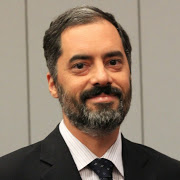
\includegraphics[width=\w,height=\h]{figs/Macri.jpg}\\
%% Lucas Macri
%% \end{textblock*}
%%   \begin{textblock*}{3cm}(7cm,2cm) % {block width} (coords)
%% 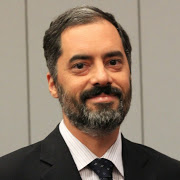
\includegraphics[width=\w,height=\h]{figs/Macri.jpg}\\
%% Wenlong Yuan
%% \end{textblock*}

  \begin{textblock*}{3cm}(5.2cm,1.35cm) % {block width} (coords)
    \textbf{Astronomers}
  \end{textblock*}
  
  \begin{textblock*}{3cm}(1.5cm,2cm) % {block width} (coords)
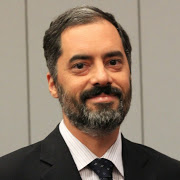
\includegraphics[width=\w,height=\h]{figs/Macri.jpg}\\
$\, \, $Lucas Macri
\end{textblock*}


  \begin{textblock*}{3cm}(5cm,2cm) % {block width} (coords)
 $\, $ 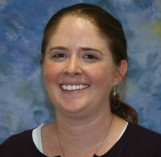
\includegraphics[width=\w,height=\h]{figs/marshall.jpg}\\
Jennifer Marshall
\end{textblock*}

  \begin{textblock*}{3cm}(8.5cm,2cm) % {block width} (coords)
 $\, $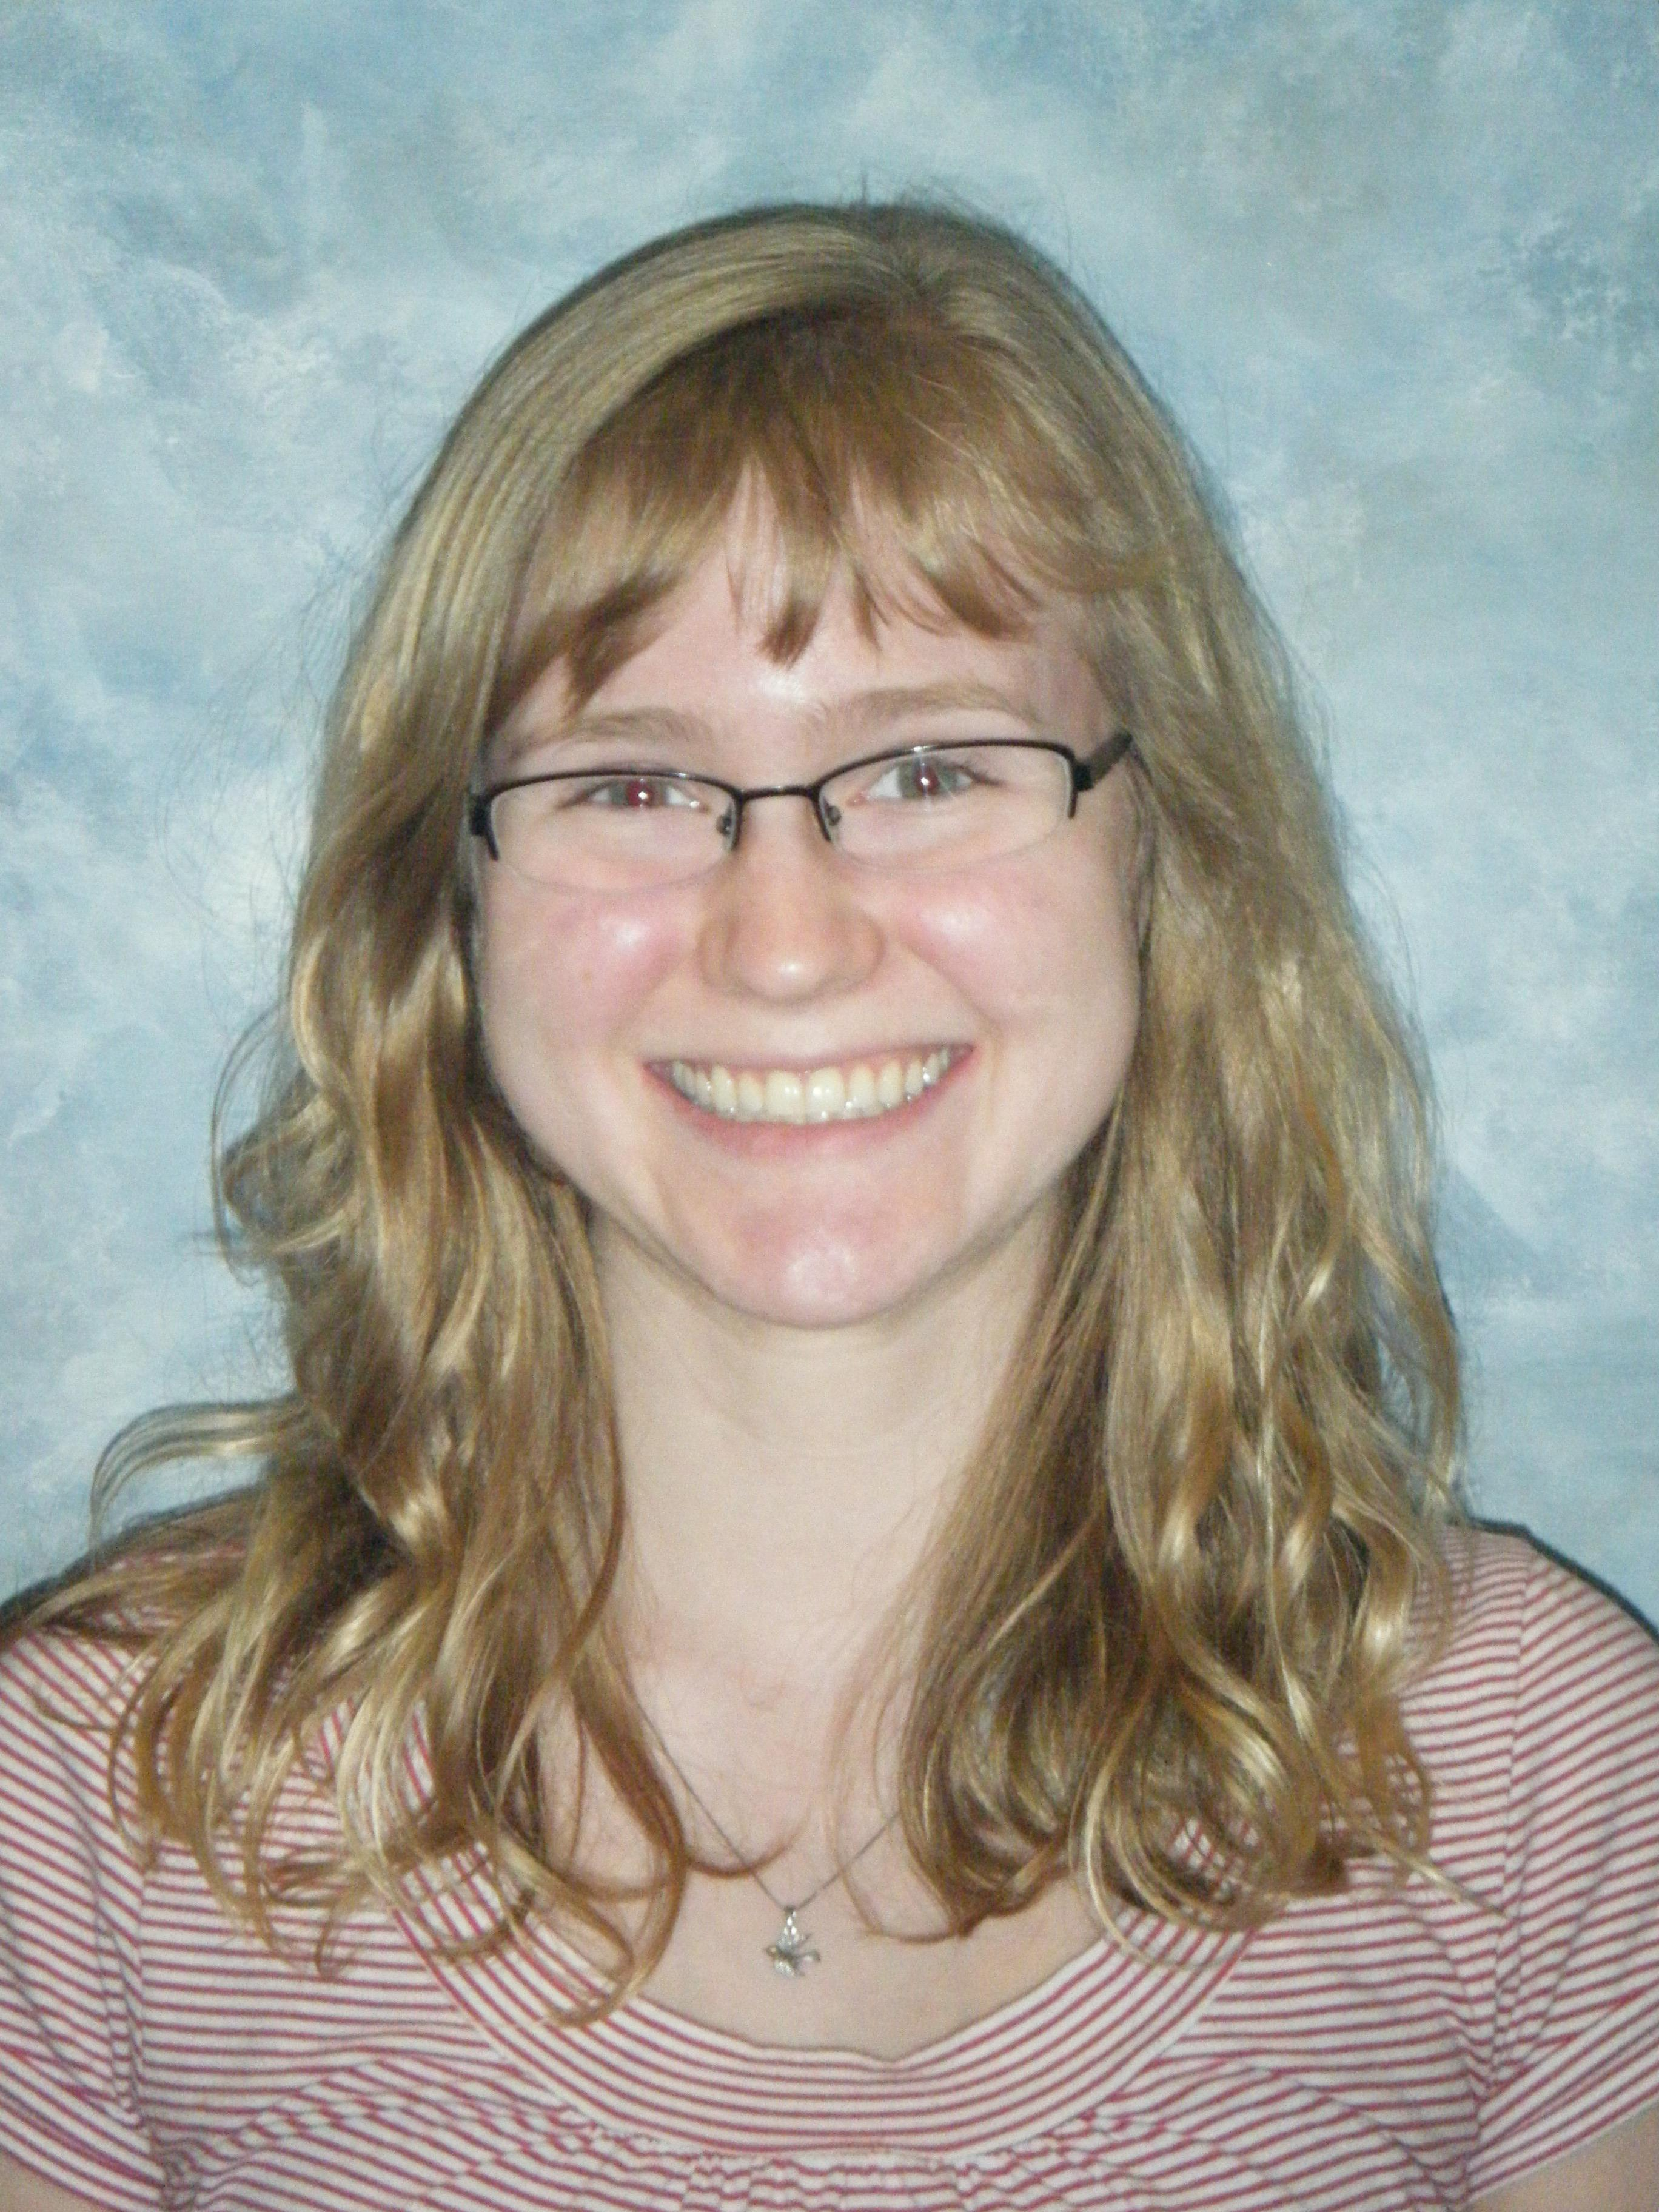
\includegraphics[width=\w,height=\h]{figs/stringer.jpg}\\
Katelyn Stringer
\end{textblock*}

  \begin{textblock*}{3cm}(2.8cm,5.5cm) % {block width} (coords)
    \textbf{Statistician}
  \end{textblock*}

  \begin{textblock*}{3cm}(2.7cm,6.25cm) % {block width} (coords)
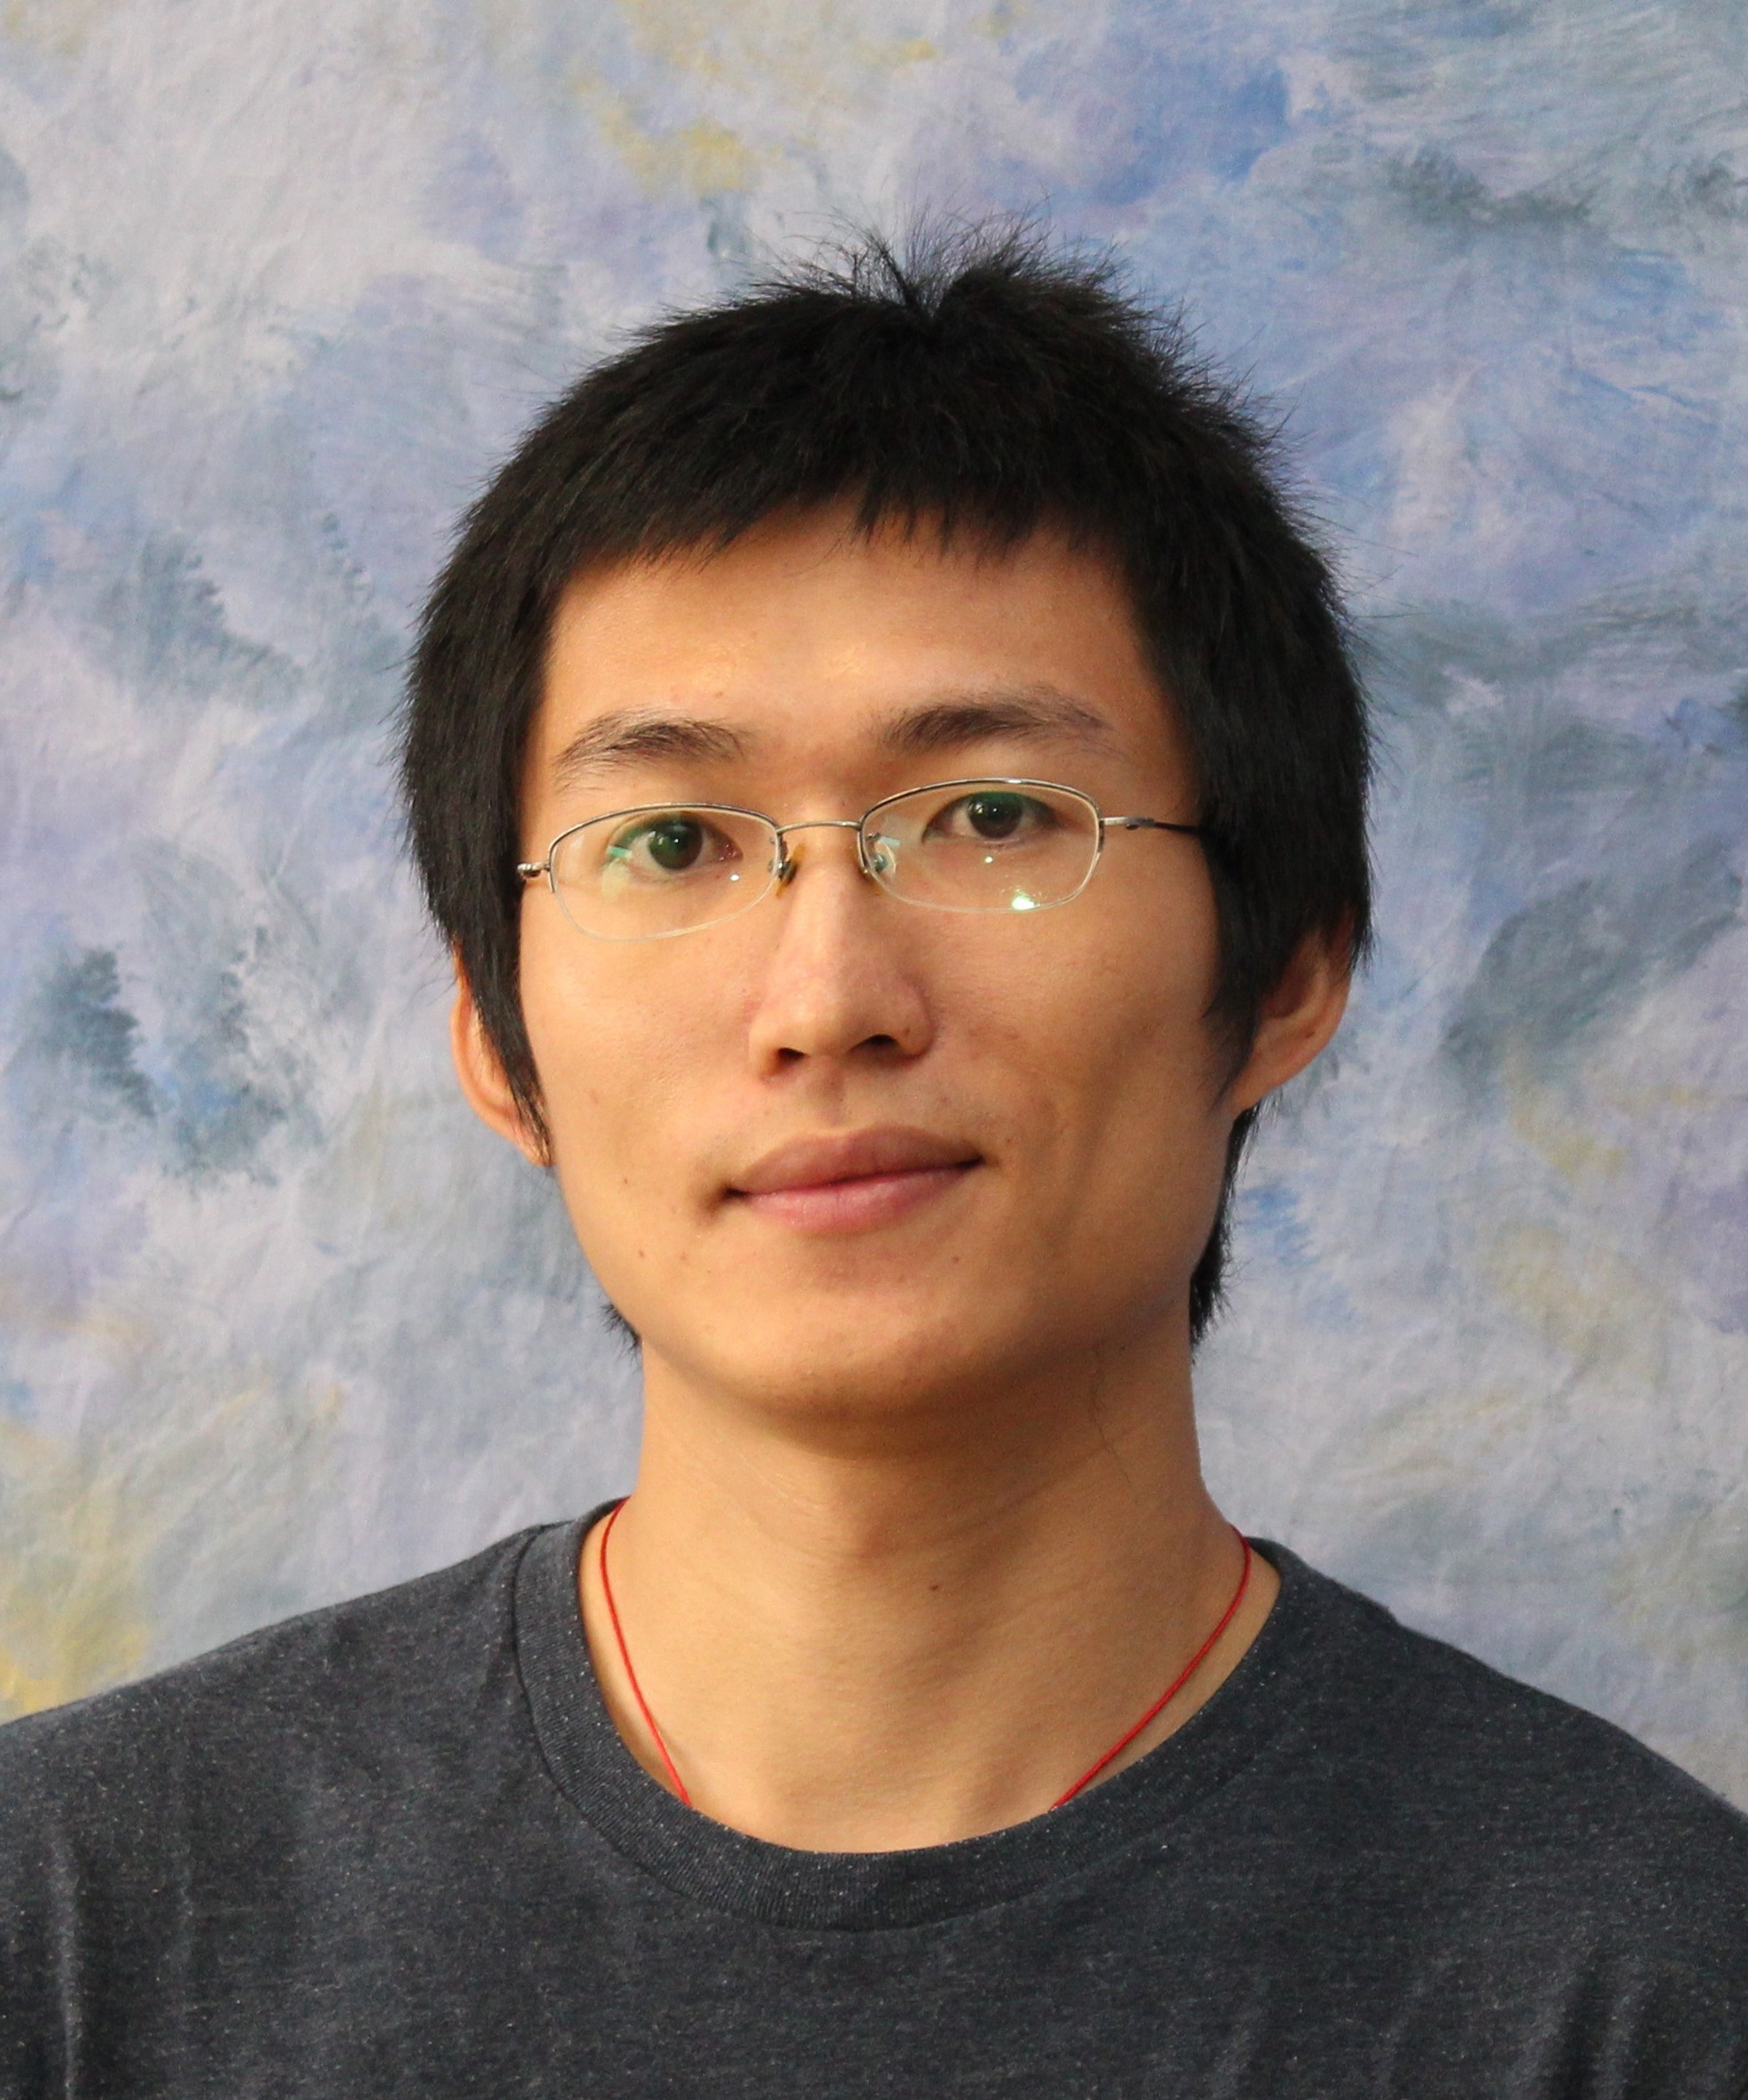
\includegraphics[width=\w,height=\h]{figs/zhenfeng.jpg}\\
$\, \, $Zhenfeng Lin
\end{textblock*}

%%   \begin{textblock*}{3cm}(5cm,6.25cm) % {block width} (coords)
%% 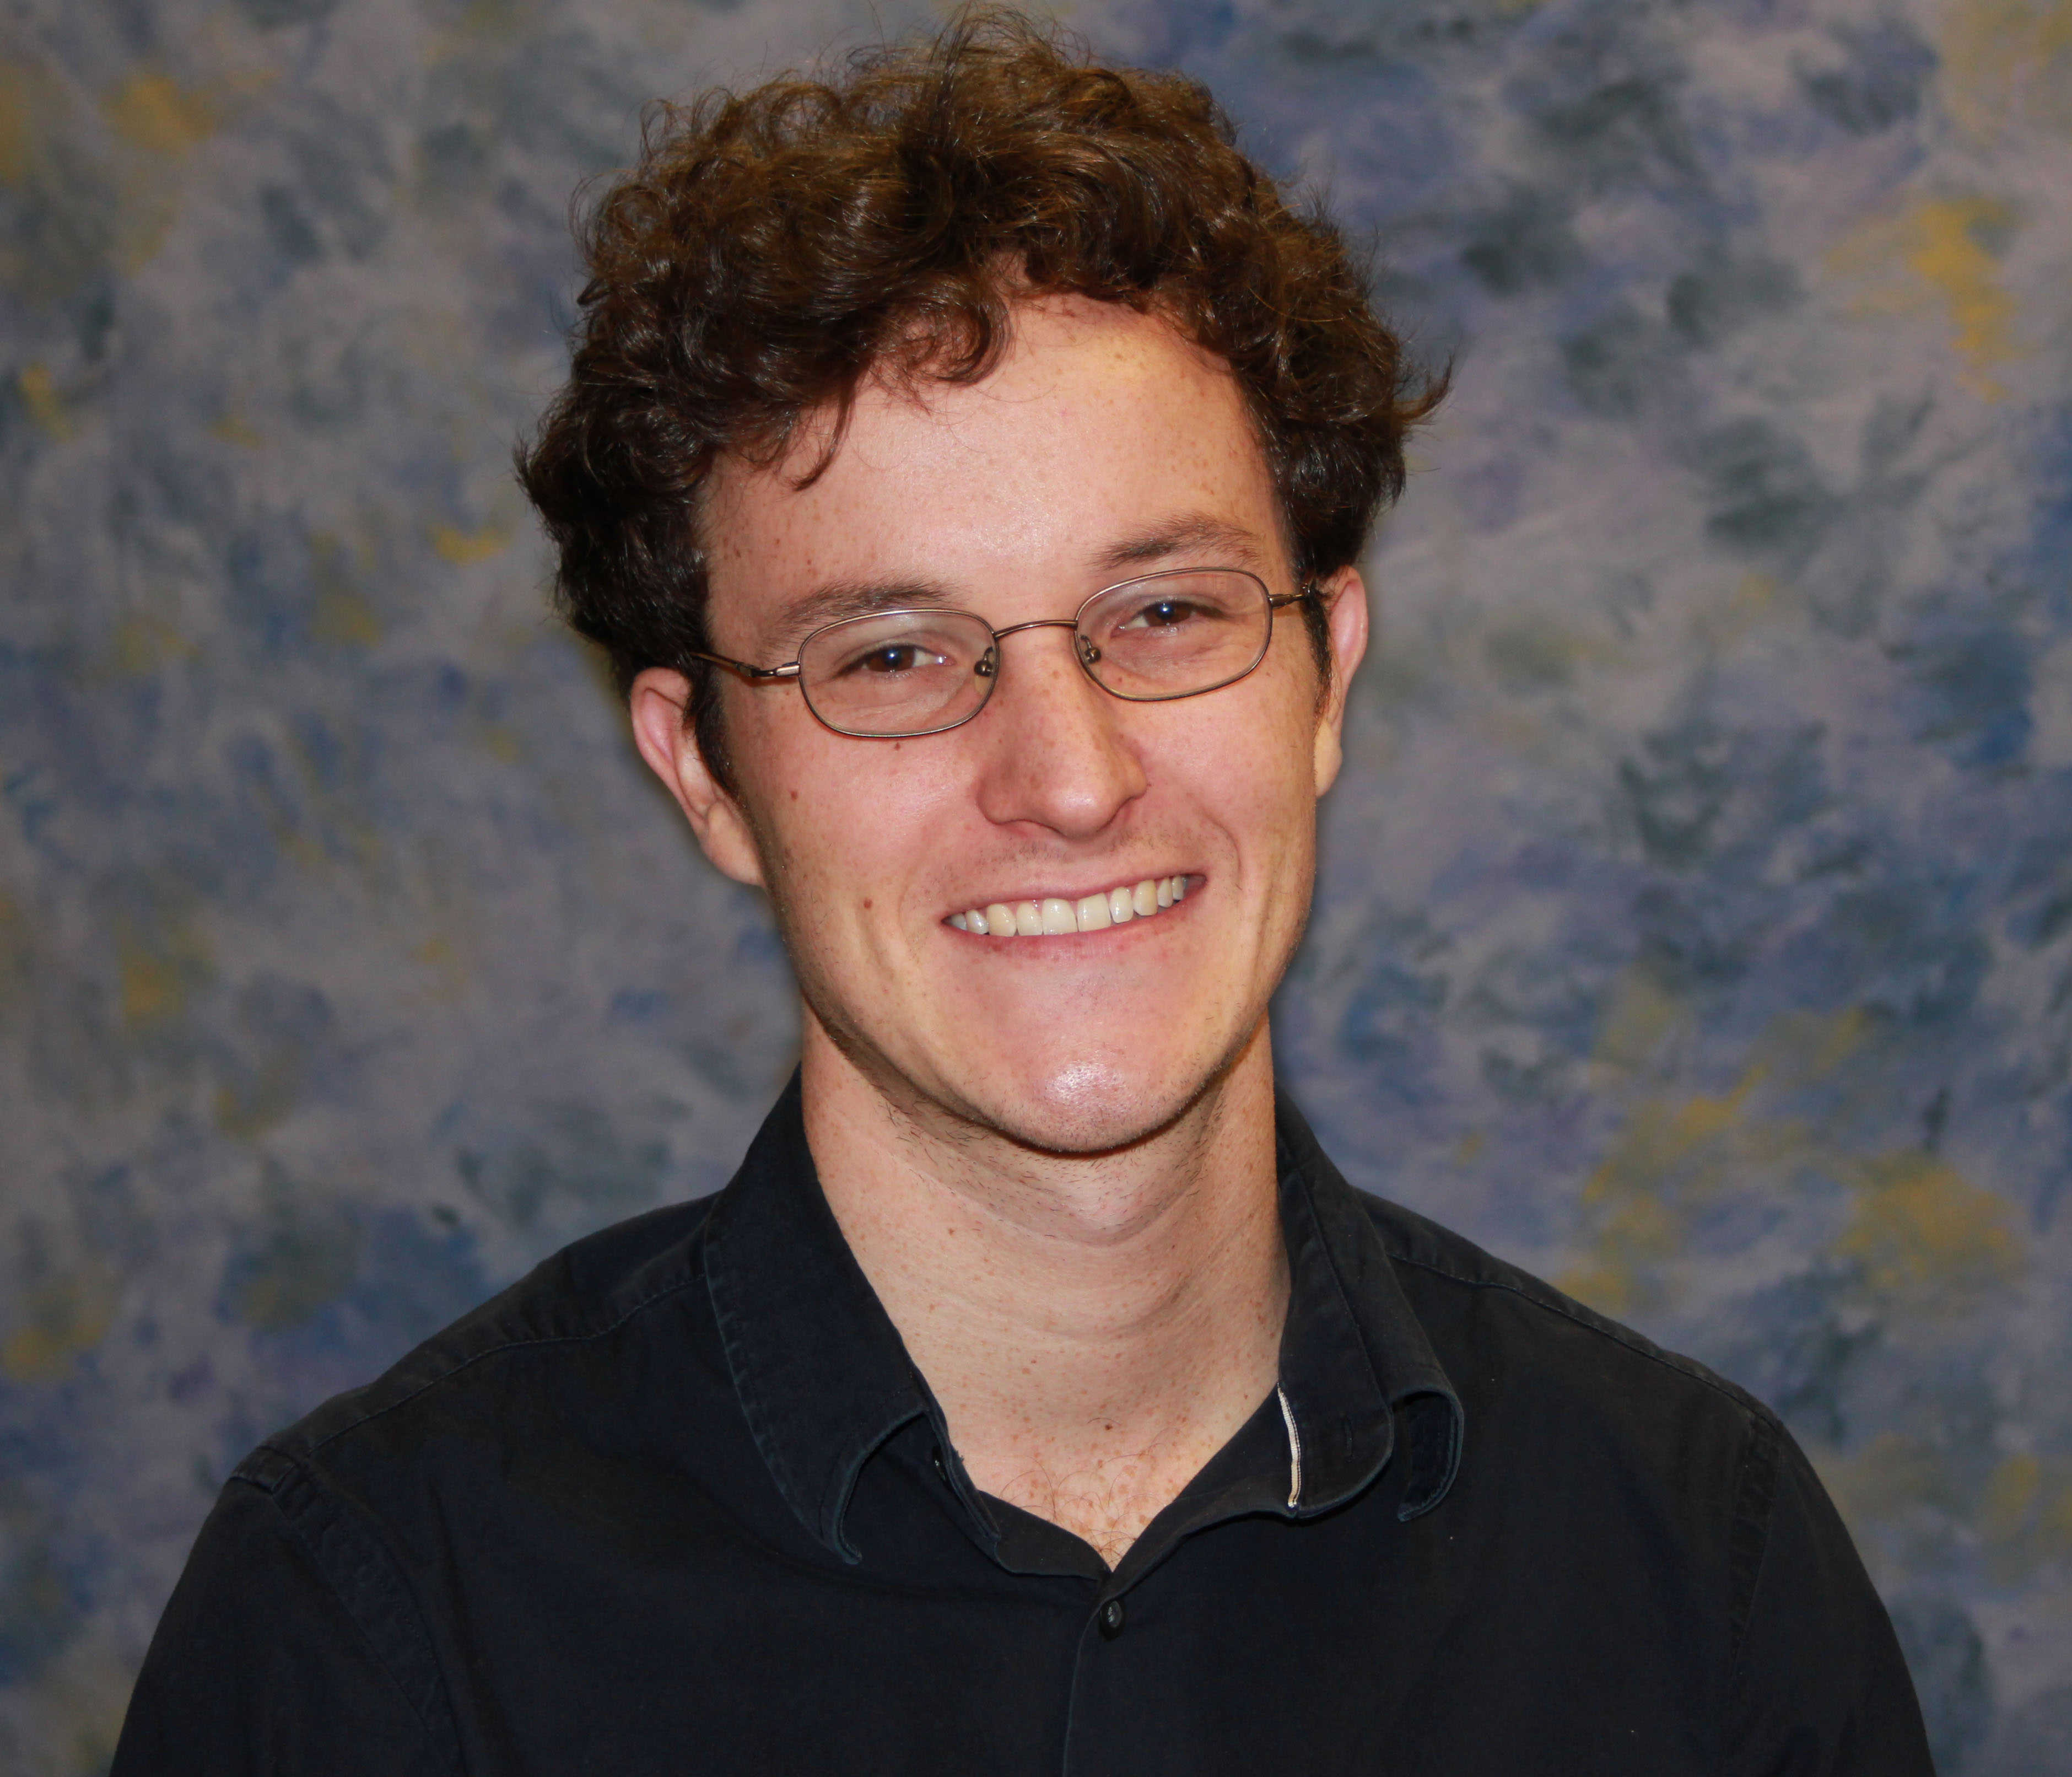
\includegraphics[width=\w,height=\h]{figs/long.jpg}\\
%% $\, \, \, $James Long
%% \end{textblock*}

  \begin{textblock*}{3cm}(6cm,6.7cm) % {block width} (coords)

\includegraphics[scale=.45]{figs/des_logo.png}\\
\end{textblock*}

  

\end{frame}


\begin{frame}{Outline}
  \tableofcontents
  \end{frame}

%\frame{\tableofcontents}

\AtBeginSection[]
{
  \begin{frame}<beamer>
    \frametitle{Outline}
    \tableofcontents[currentsection,currentsubsection]
  \end{frame}
}

\AtBeginSubsection[]
{
  \begin{frame}<beamer>
    \frametitle{Outline}
    \tableofcontents[currentsection,currentsubsection]
  \end{frame}
}



%%%%%%%%
%%%%%%%% TODO: redo first section with more emphasis on multiband, lomb scargle
%%%%%%%%



\section{Distance Determination, Variable Stars, Milky Way Halo}

\begin{frame}{What is the distance to these objects?}

  \begin{center}
    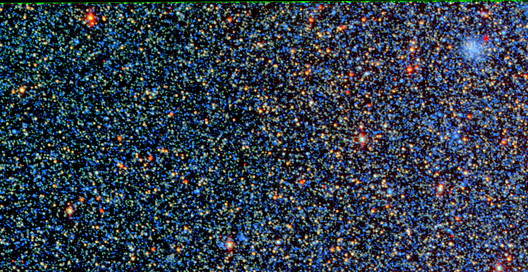
\includegraphics[scale=0.5]{figs/des_small.png}\\
  \end{center}
  \textbf{Problem:}
  \begin{equation*}
    \text{ brightness } \propto \frac{\text{luminosity}}{\text{distance}^2}
  \end{equation*}
\begin{center}
  Only brightness can be directly measured.
  \end{center}

\foot{Image Source: DES Collaboration}
\end{frame}

\begin{frame}{Standard Candles}
  \textbf{Standard Candles:} Class of objects with same luminosity
  \begin{itemize}
  \item Know absolute luminosity of standard candle.
  \item Determine object is standard candle and estimate its brightness.
  \end{itemize}

  \vspace{.3in}
  
  \textbf{RR Lyrae (RRL):} Standard candle variable star
  \begin{itemize}
  \item All RR Lyrae have (approximately) same luminosity
  \end{itemize}
\end{frame}

\begin{frame}{RR Lyrae Variable Star}
\textbf{Periodic variables:} Stars that repeat brightness variation over a fixed period.
\begin{center}
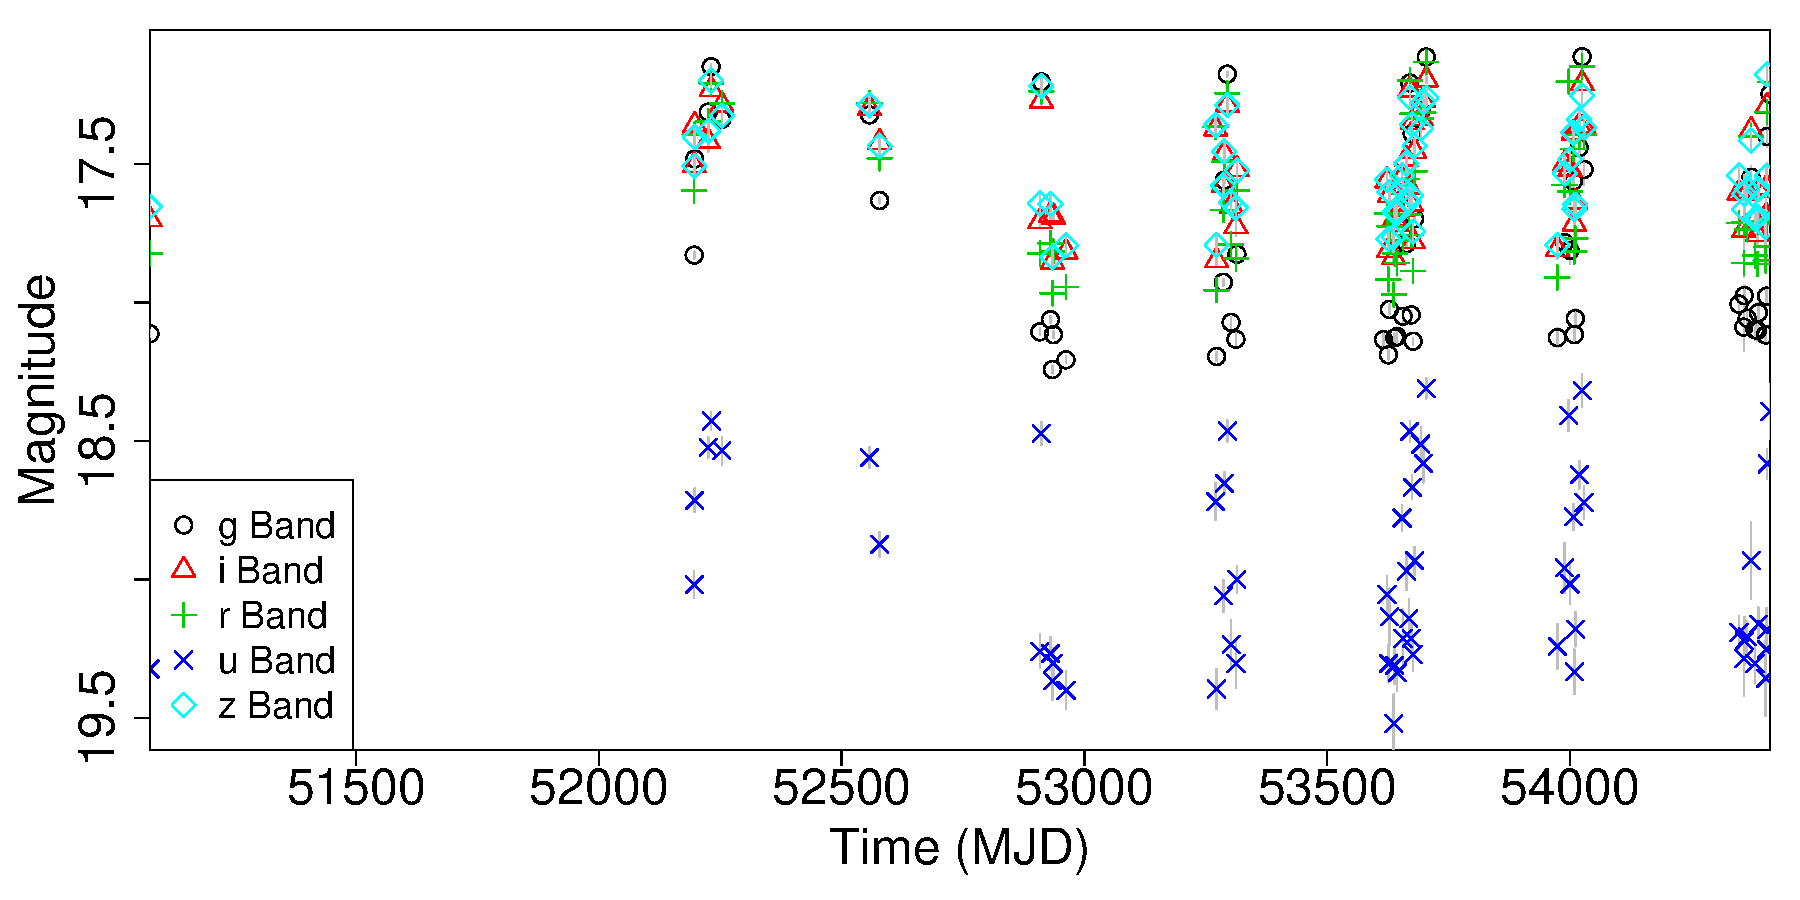
\includegraphics[scale=.3]{figs/unfolded_13350.pdf}
\end{center}


  \begin{itemize}
    \item Star observed $\approx 250$ times in $5$ bands ($u,g,r,i,z$).
    \item Known as a \textit{light curve}.
  \end{itemize}

%% \begin{itemize}
%% \item Star observed $\approx 250$ times in $5$ bands, $u,g,r,i,z$.
%% \item Data for star is $D=\{t_{jb},m_{jb},\sigma_{jb}\}_{j=1}^{n_b}$ for $b=1,\ldots,B$.
%% \item Observe brightness $m_{jb}$ at time $t_{jb}$ with uncertainty $\sigma_{jb}$ in band $b$.
%% \end{itemize}
\end{frame}


\begin{frame}{Folded Light Curve of RR Lyrae}
\textbf{Folded light curve:} Brightness versus time modulo period.
\begin{center}
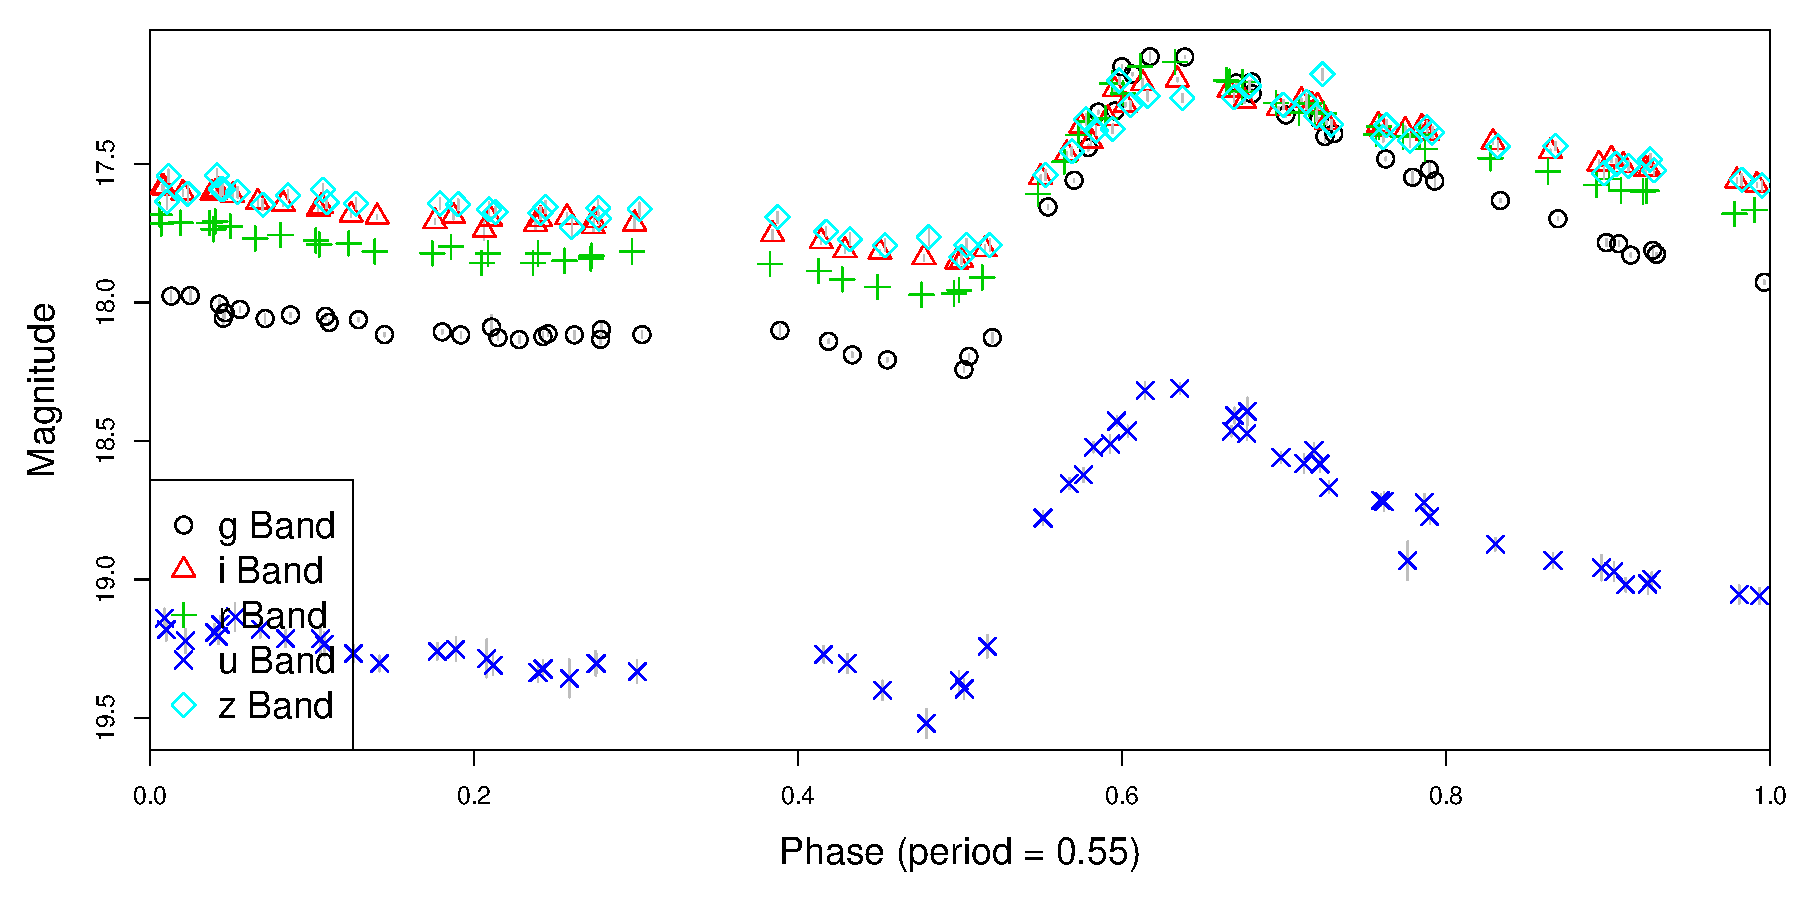
\includegraphics[scale=.3]{figs/folded_13350.pdf}\\
Distance to this star is proportional to mean magnitude, after accounting for \underline{dust} and \underline{PL relation}.
\end{center}
\end{frame}


\begin{frame}{Sloan Digital Sky Survey (SDSS) III -- Stripe 82}
\begin{itemize}
\item Discovered $\approx 60,000$ variable stars
\item $\approx 250$ brightness measurements / star
\item Variables belong to different \textbf{classes}
\end{itemize}


  \begin{center}
    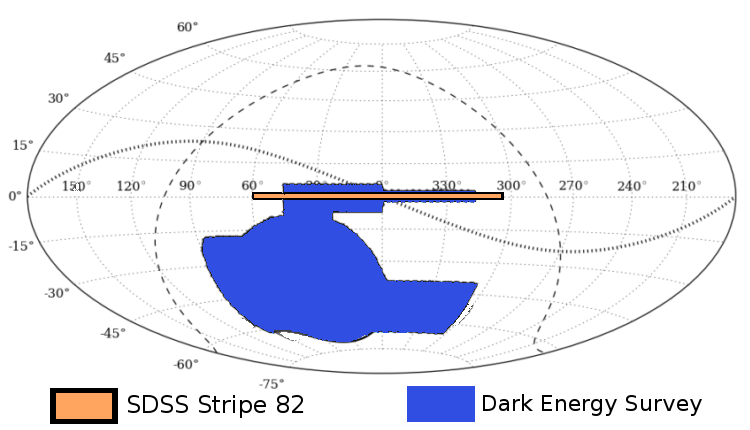
\includegraphics[scale=0.2]{figs/des_observing_strategy.png}
    \end{center}


%\underline{Example Light Curve}
%\vspace{-.1in}
\begin{center}
Example Light Curve: Eclipsing Binary (Unfolded and Folded)\\
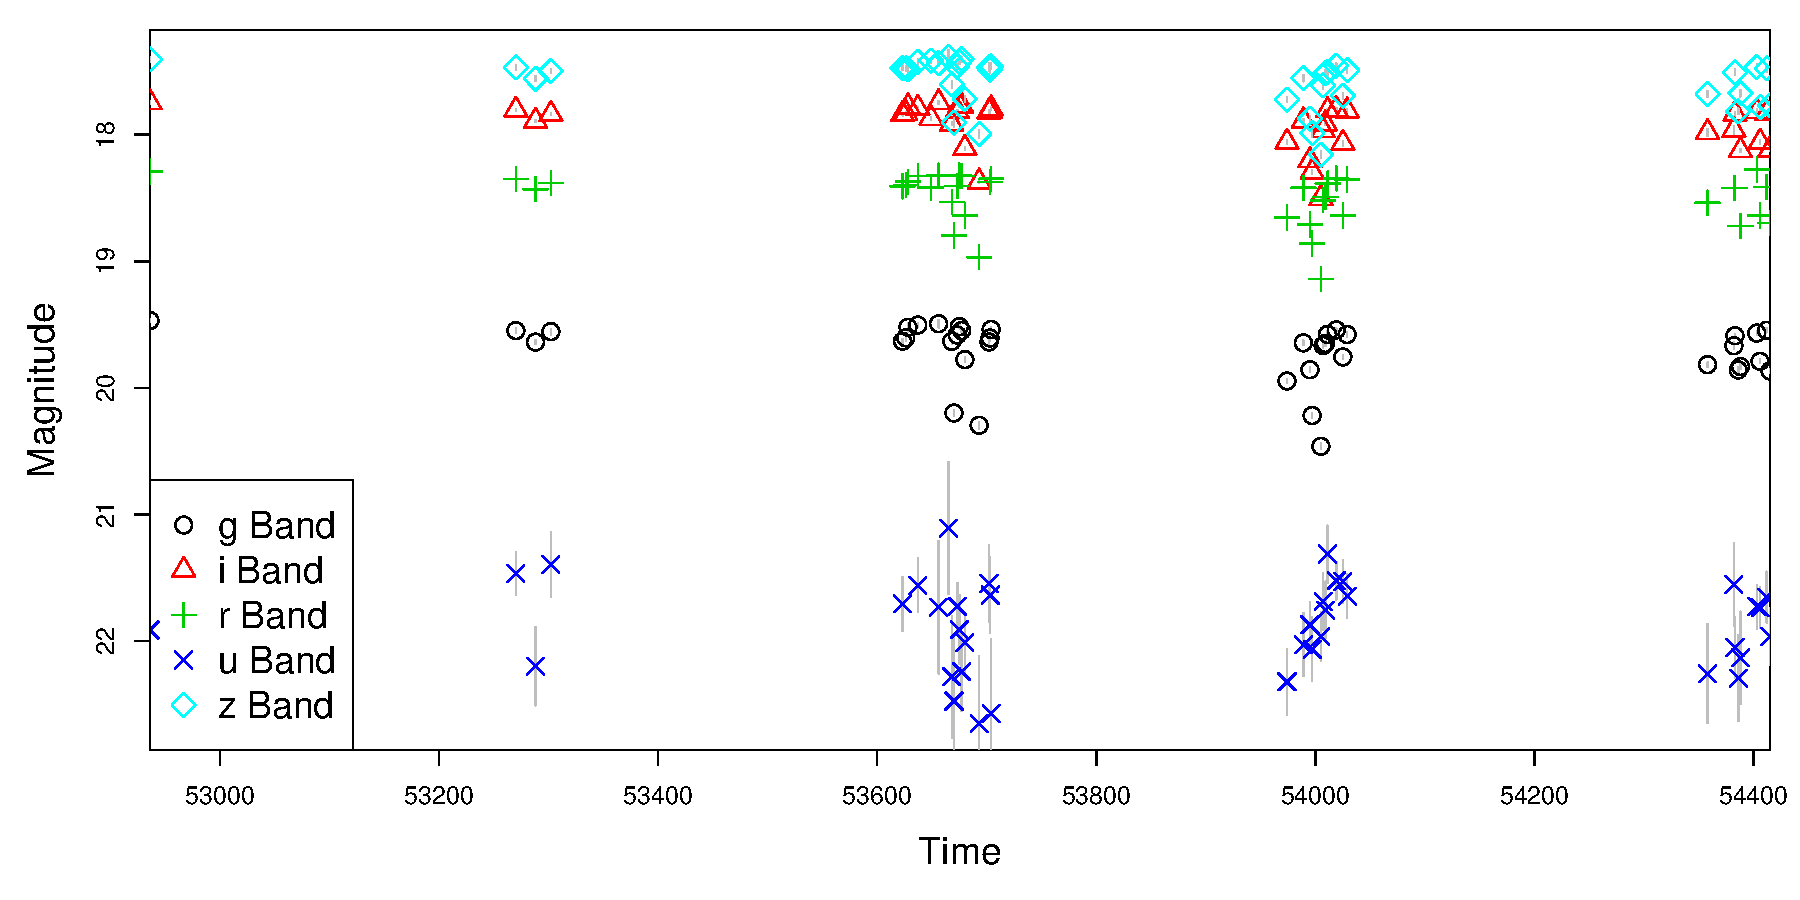
\includegraphics[scale=.15]{figs/unfolded_4183016.pdf}
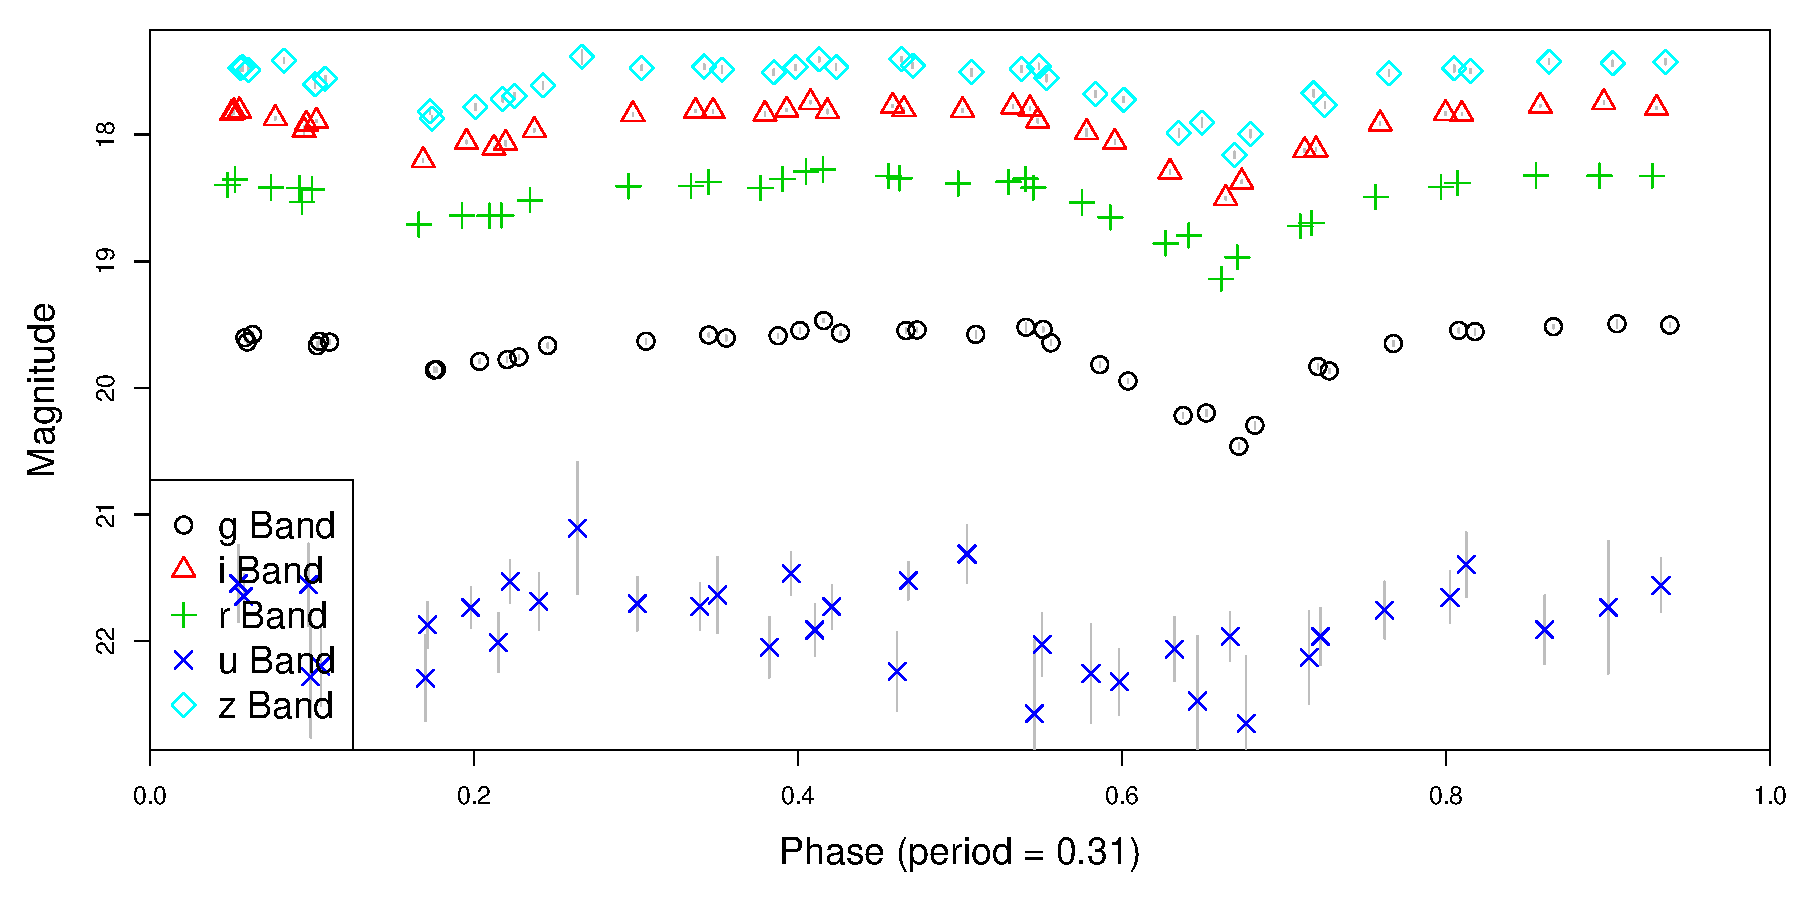
\includegraphics[scale=.15]{figs/folded_4183016.pdf}
\end{center}

\att{See Ivezic \cite{ivezic2007sloan}}

\end{frame}




%% \begin{frame}{SDSS--III Stripe 82}
%% \begin{itemize}
%% \item Discovered $\approx 60,000$ variables
%% \item Variables belong to different \textbf{classes}
%% \item Some periodic, some not
%% \end{itemize}

%% \underline{Three Examples}

%% \vspace{-.1in}

%% \begin{center}
%% {\small 1) Eclipsing Binary (Unfolded and Folded)}\\
%% 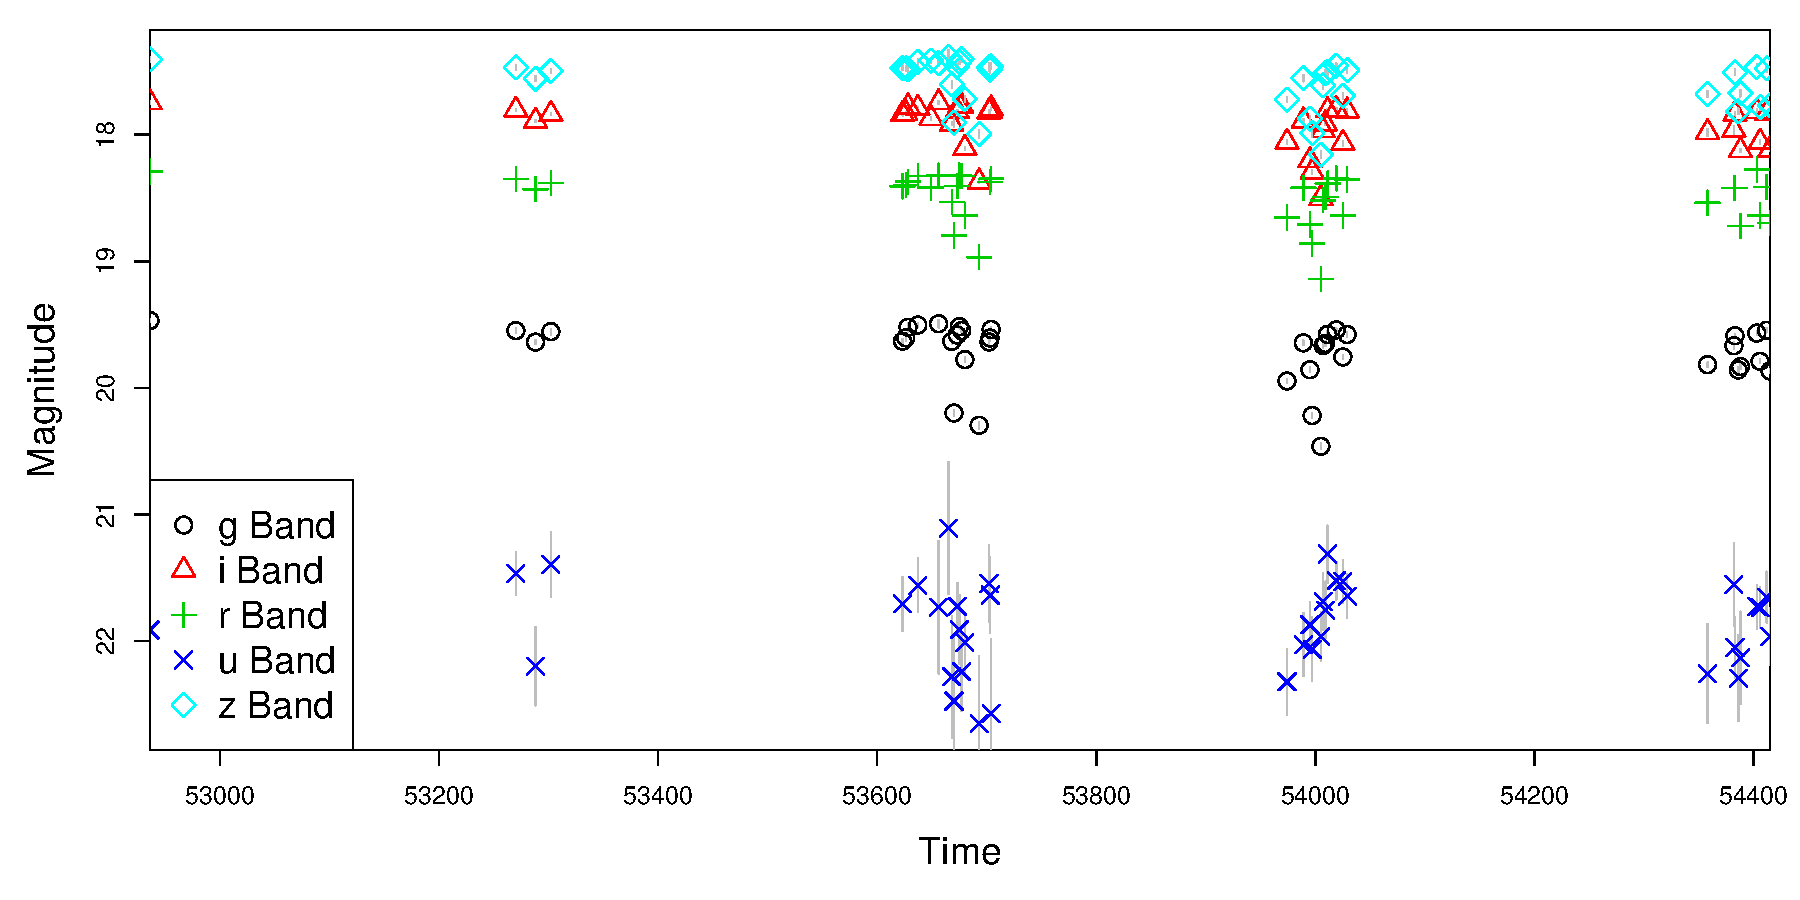
\includegraphics[scale=.15]{figs/unfolded_4183016.pdf}
%% 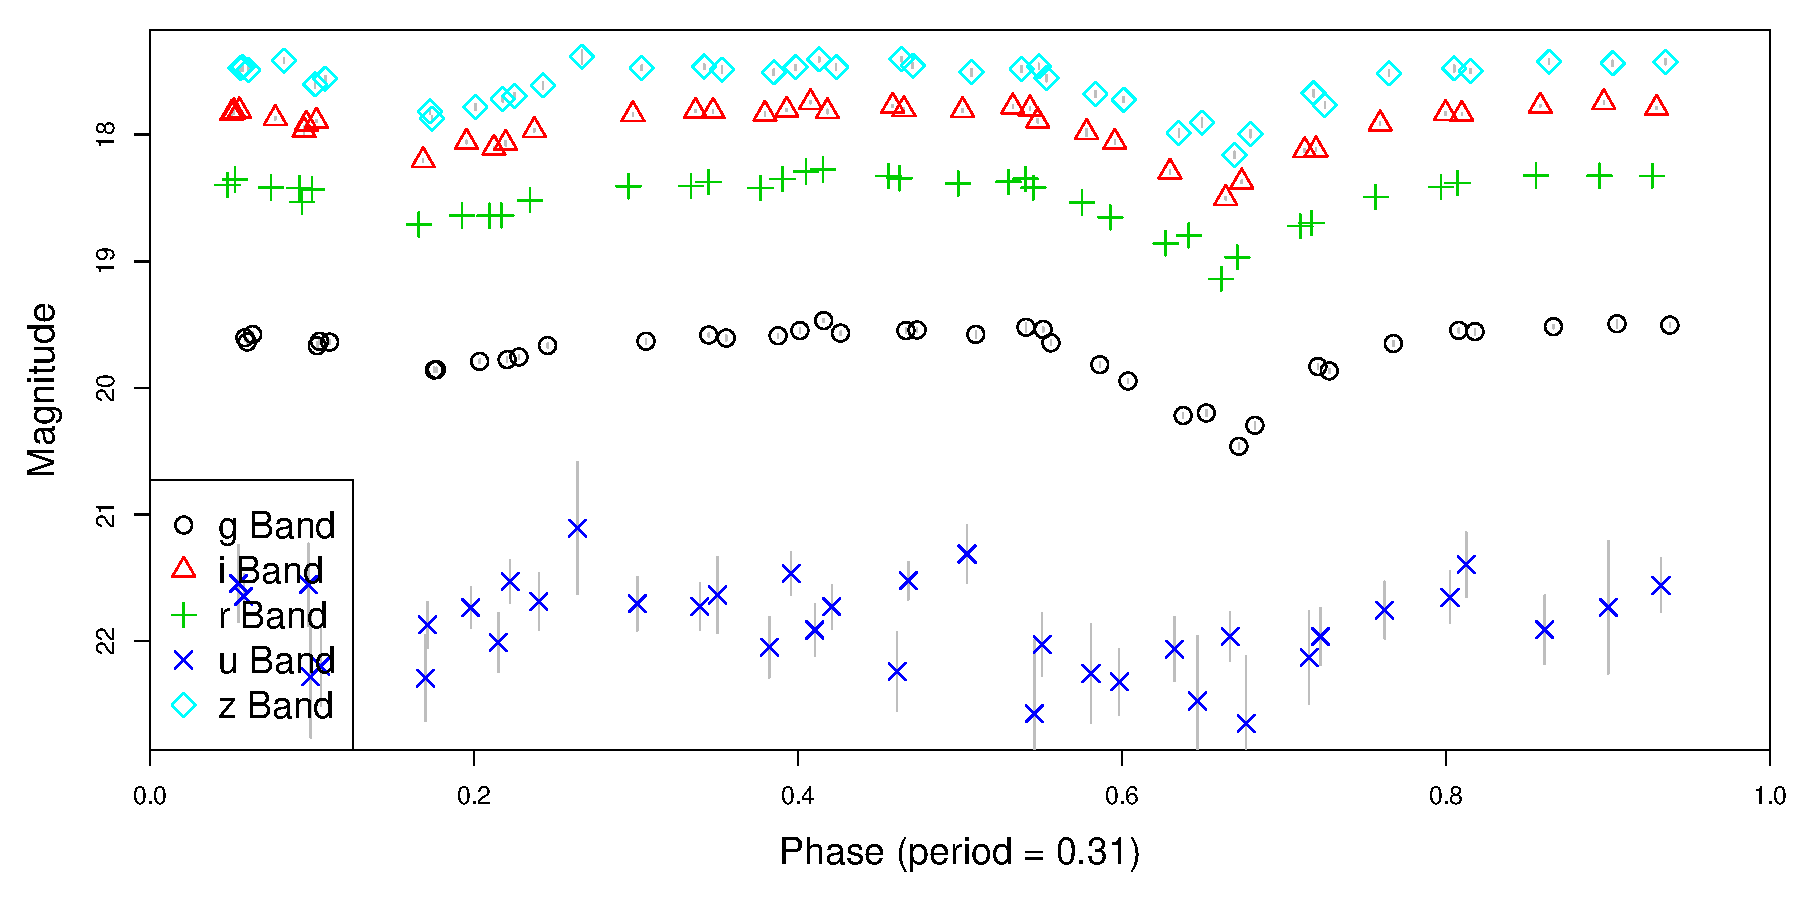
\includegraphics[scale=.15]{figs/folded_4183016.pdf}
%% \end{center}

%% \vspace{-.2in}

%% %% \begin{center}
%% %% RR Lyrae\\
%% %% 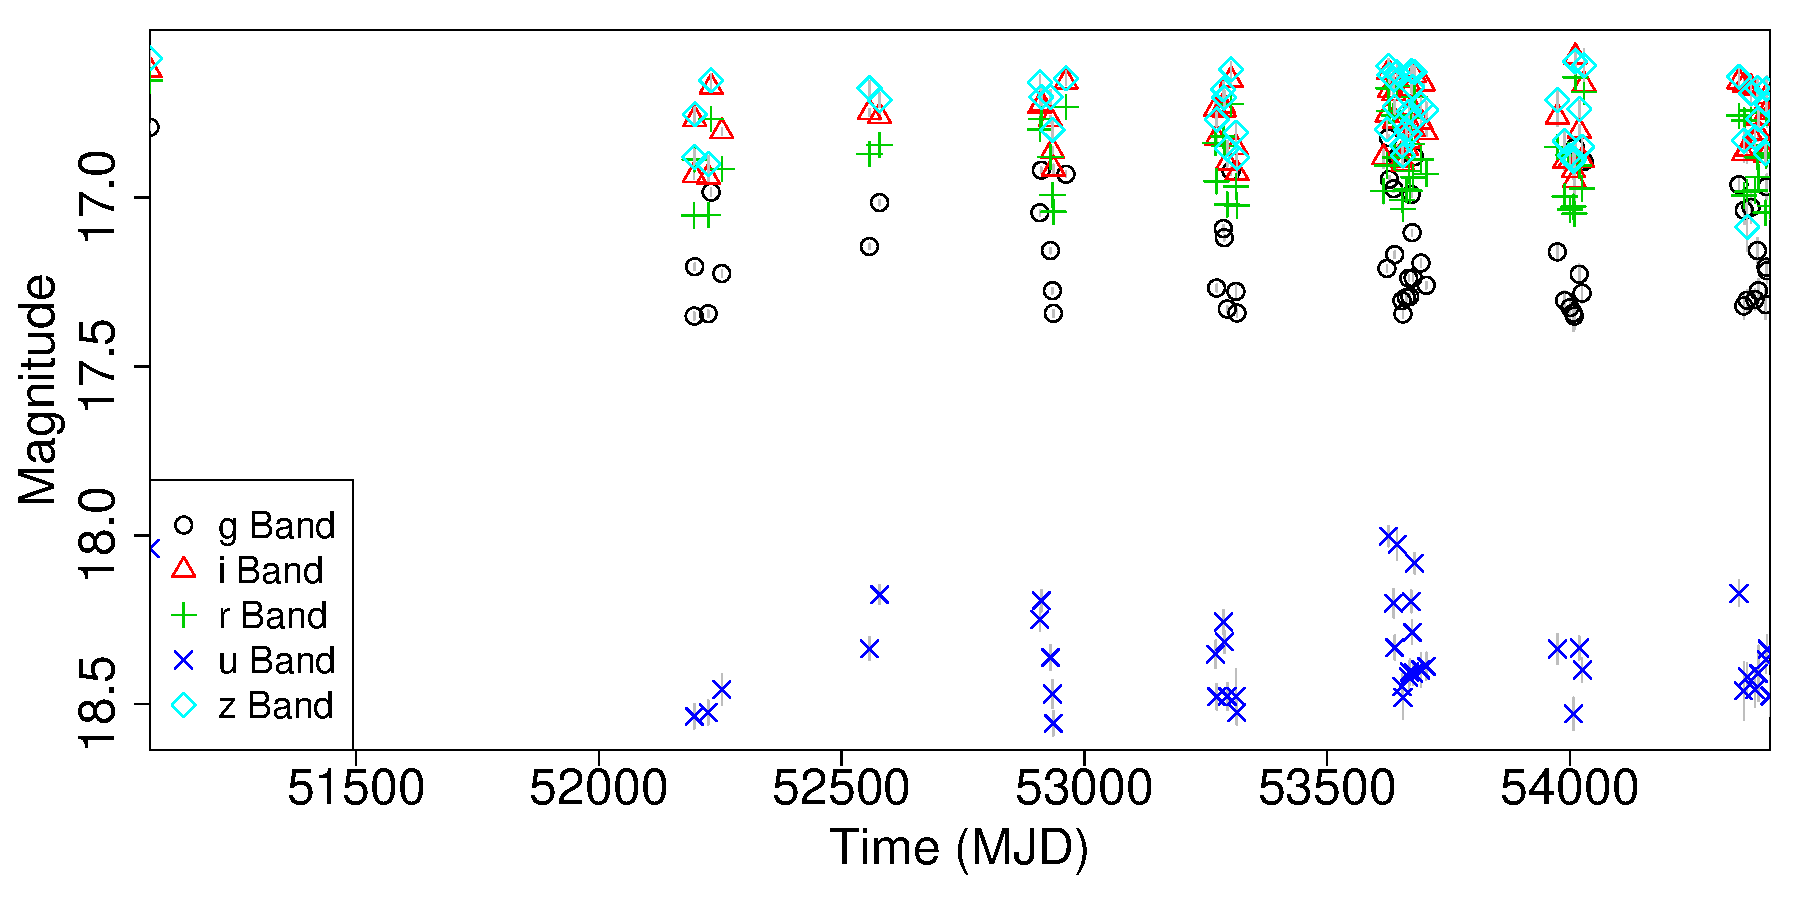
\includegraphics[scale=.15]{figs/unfolded_4099.pdf}
%% %% 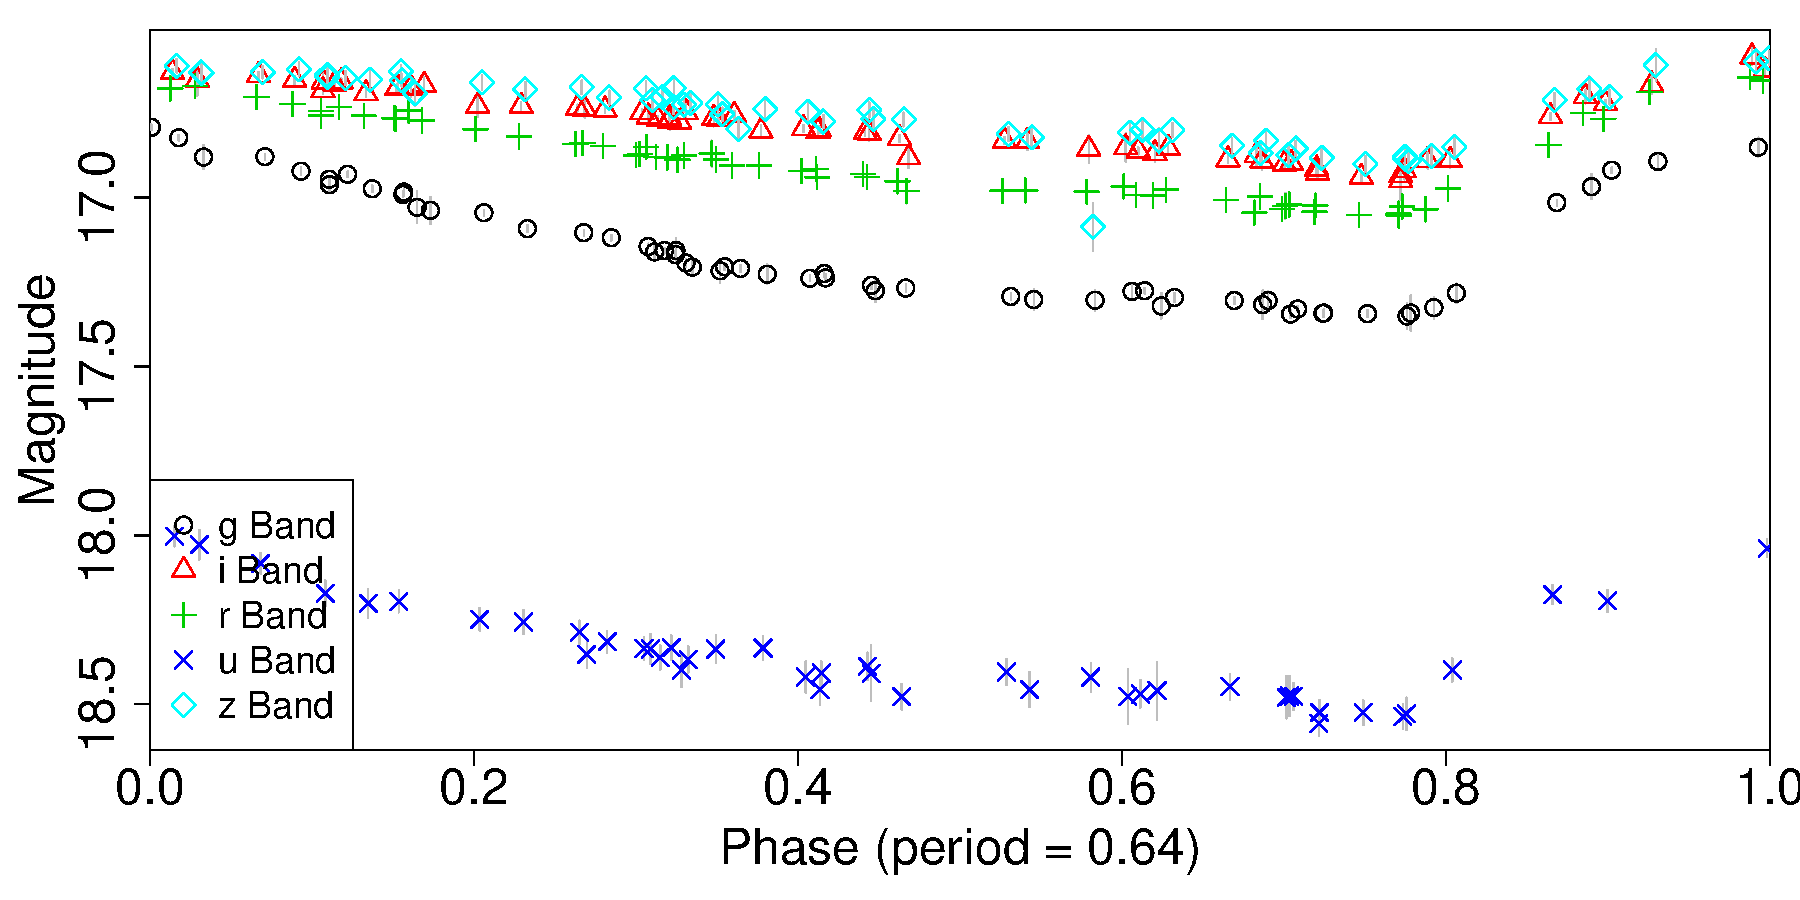
\includegraphics[scale=.15]{figs/folded_4099.pdf}
%% %% \end{center}


%% \begin{center}
%% {\small 2) Quasar (unfolded)} \hspace{9 mm} {\small 3) RR Lyrae (folded)}\\
%% 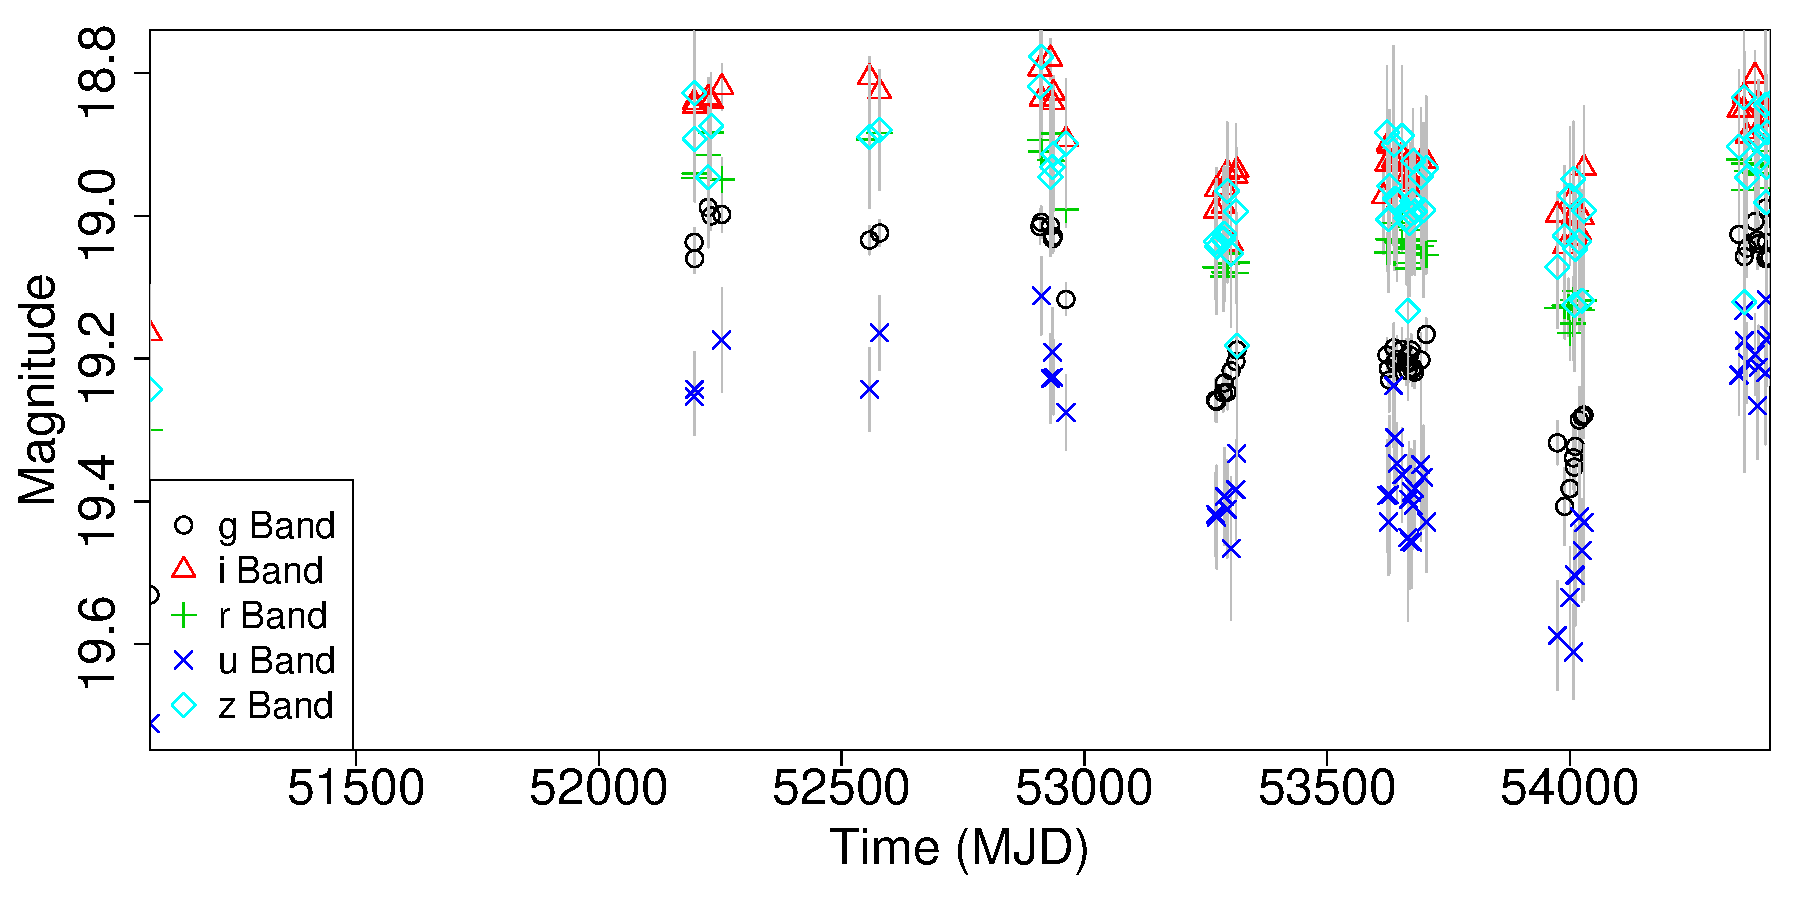
\includegraphics[scale=.15]{figs/unfolded_7904669.pdf}
%% 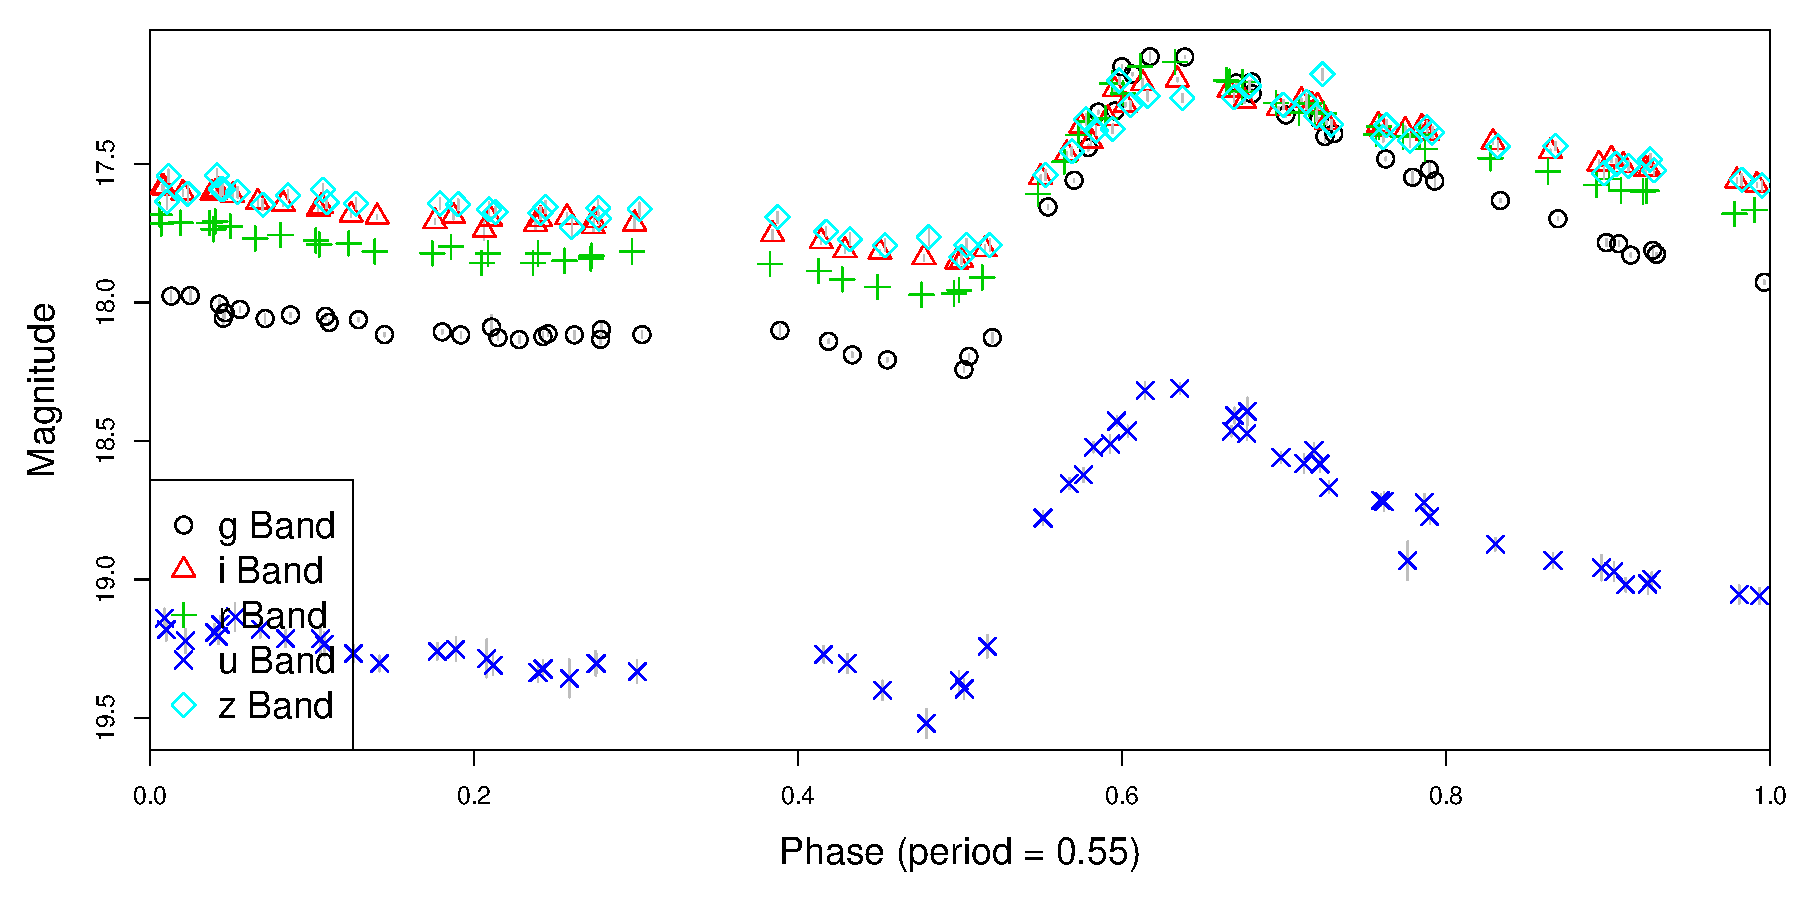
\includegraphics[scale=.15]{figs/folded_13350.pdf}
%% \end{center}

%% \att{See Ivezic \cite{ivezic2007sloan}}

%% \end{frame}

\begin{frame}{Identifying RRL, Mapping MW Halo with SDSS}
  Sesar 2010:
  \begin{enumerate}
  \item Extracted features for $\approx 60,000$ variables (eg period, amplitude)
  \item Identified $\approx 350$ RR Lyrae
  \item Estimated Distances to RRL
  \end{enumerate}

  \begin{columns}
    \begin{column}{0.5\textwidth}

      \vspace{-.22in}

      \begin{center}
        \underline{Steps 1 and 2}
        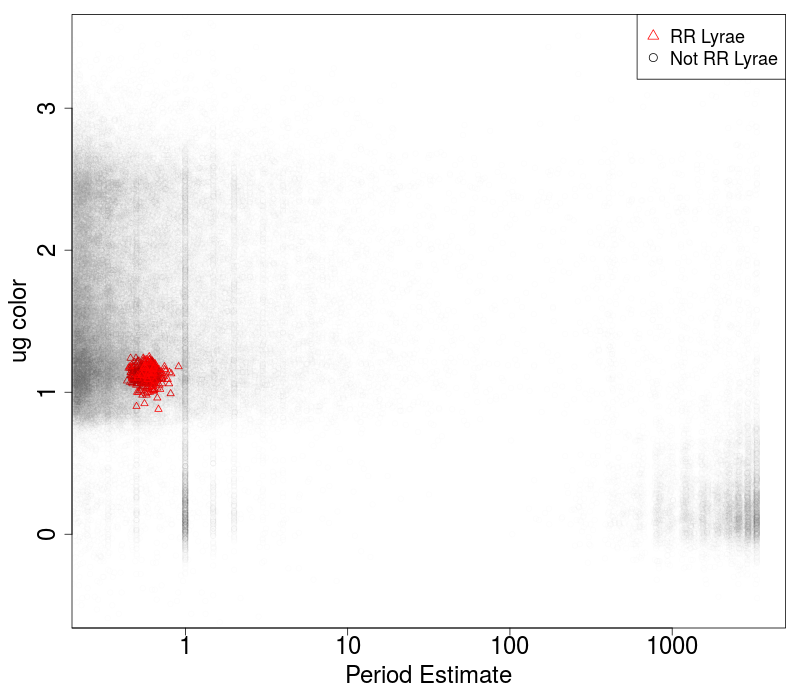
\includegraphics[scale=.2]{figs/sdss_color_period.png}
      \end{center}
      \end{column}
    \begin{column}{0.5\textwidth}

      \vspace{-.55in}

      \begin{center}
      \underline{Step 3}
      \end{center}
      
      \vspace{-.35in}
      \begin{center}
      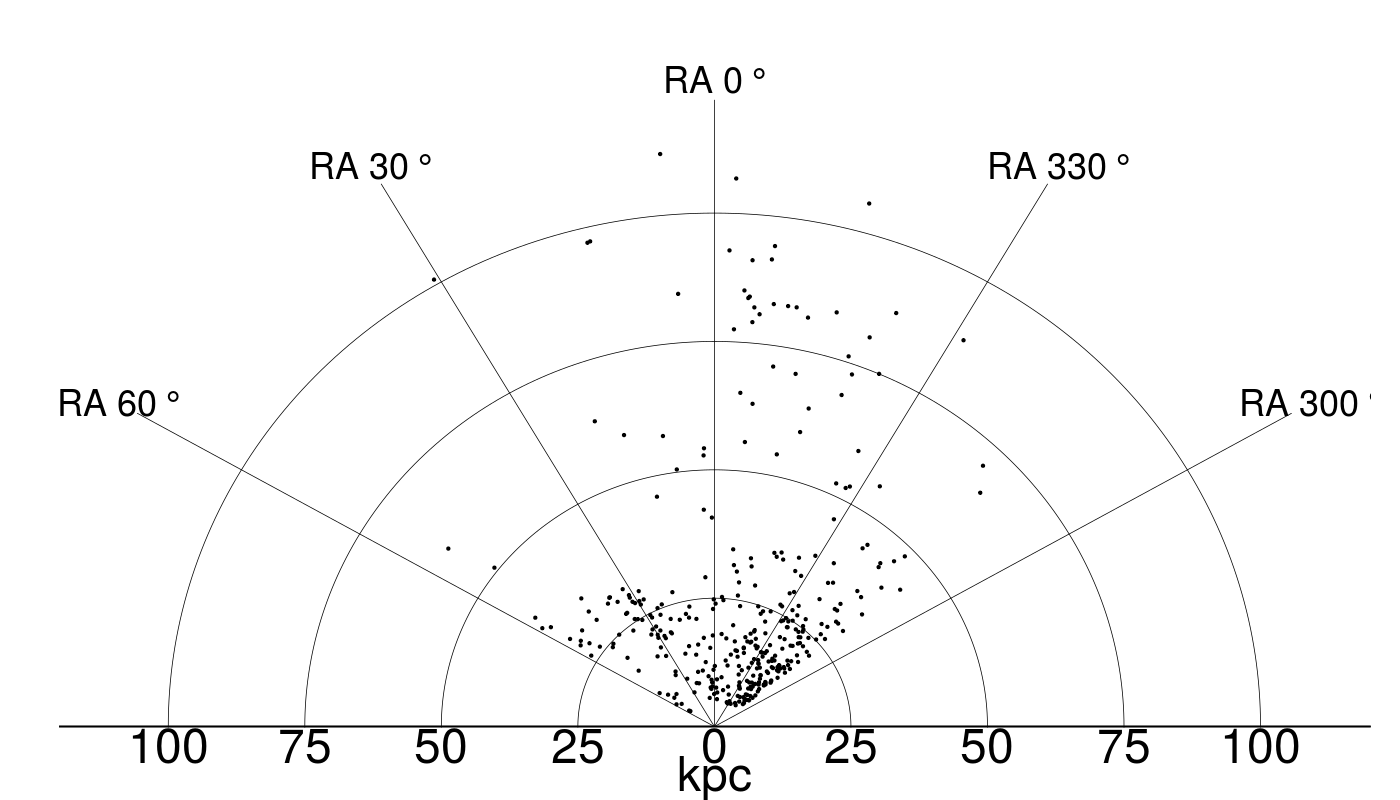
\includegraphics[scale=.1]{figs/density_true_points.png}\\
      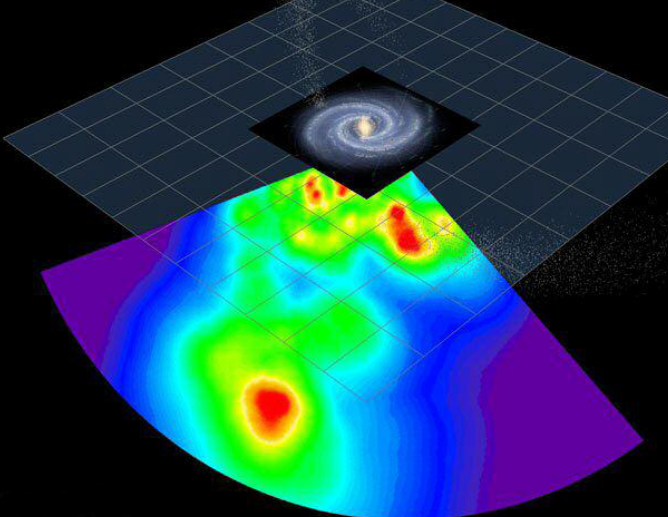
\includegraphics[scale=.17]{figs/sesar_map.png}
      \end{center}
    \end{column}
\end{columns}

\att{Sesar 2010 \cite{sesar2010light}}
  
\end{frame}

%% \begin{frame}{Importance of MW Halo Maps}
%% \todo{compare cosmological simulations to observed structure}
%% \end{frame}

%% \begin{frame}{Mapping Milky Way Halo with RRL}

%%   \begin{center}
%%     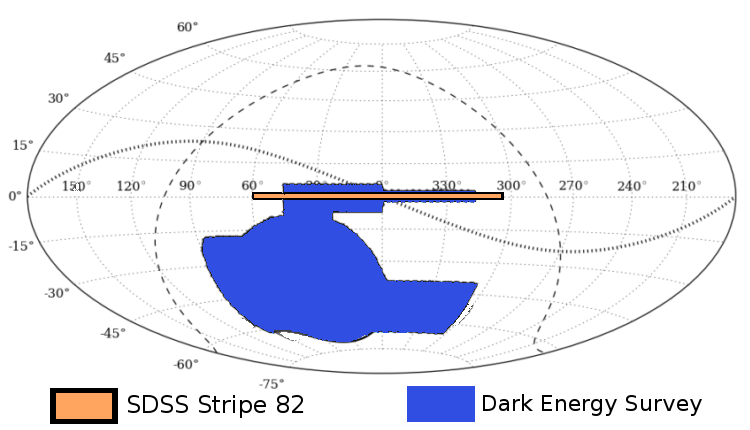
\includegraphics[scale=0.2]{figs/des_observing_strategy.png}
%%     \end{center}
  
%% \begin{center}
%%   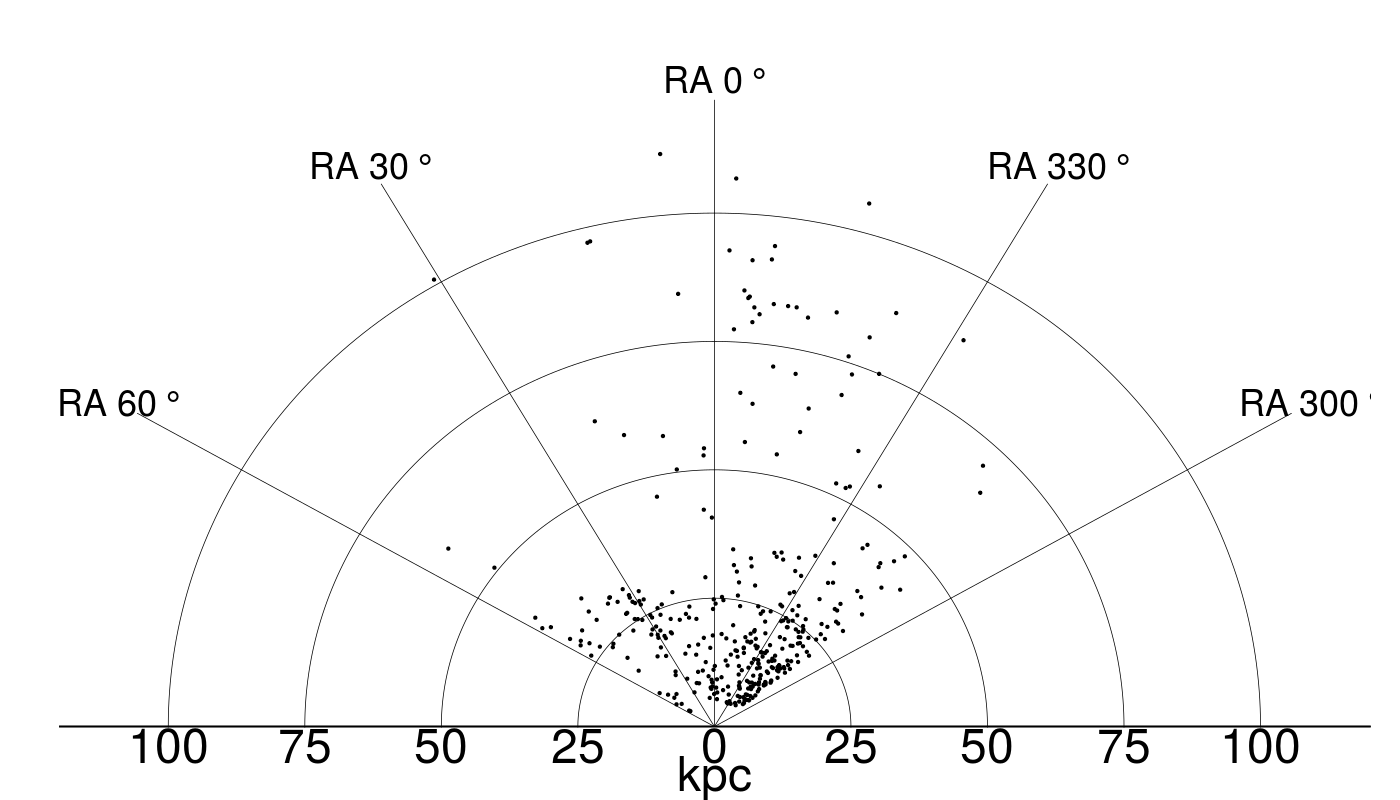
\includegraphics[scale=.13]{figs/density_true_points.png}\\
%%   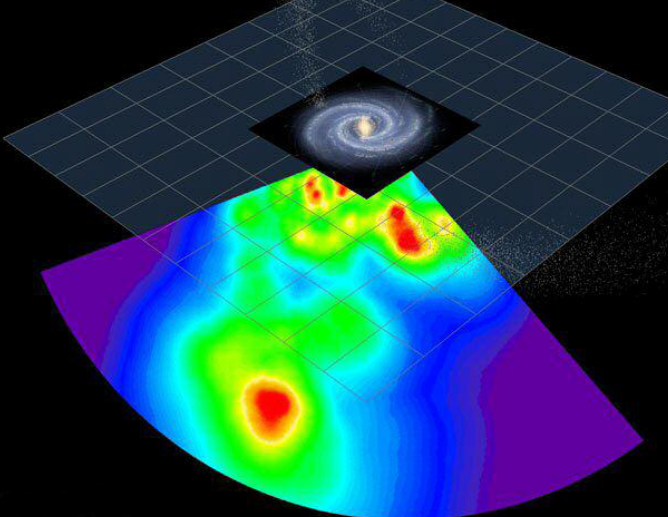
\includegraphics[scale=.2]{figs/sesar_map.png}
%% \end{center}

%% %% \begin{itemize}
%% %% \item Compare maps to cosmological simulations.
%% %% \item Answer missing satellites problem.
%% %% \end{itemize}

%% \att{Sesar \cite{sesar2010light}}

%% \end{frame}




%% \begin{frame}{Mapping the Galactic Halo: Statistical Challenges}
%% \begin{itemize}
%% \item Classification: Identify RR Lyrae lightcurves.
%% \item Parametric Inference: Estimate periods, mean magnitudes, distances.
%% \item Nonparametric Inference: Construct 3--D density map.
%% \end{itemize}
%% \end{frame}

%% \begin{frame}{The Dark Energy Survey}
%% \todo{picture of telescope}
%% \end{frame}


\begin{frame}{Mapping the Galactic Halo with DES}

\textbf{Dark Energy Survey (DES)}
\begin{itemize}
\item $\approx$ 10 photometric measurements in ($g$,$i$,$r$,$z$,$Y$) over five years
\item 68 million stars
\item depths to 24 mag in $i$
\item 5000 square degrees ($\approx$ 1/9$^{th}$ entire sky)
\end{itemize}

\vspace{.1in}
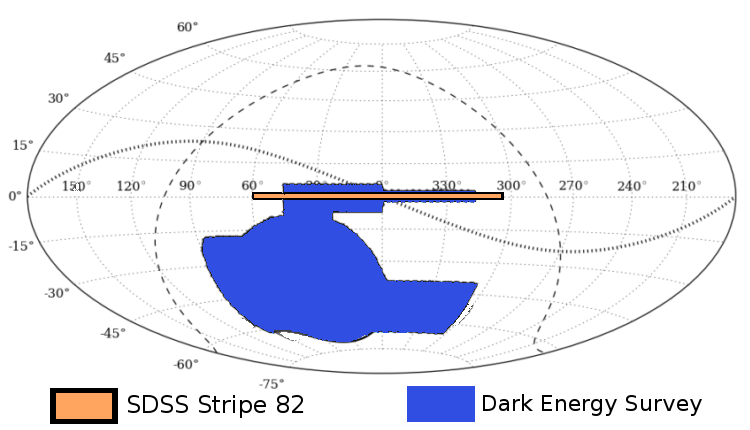
\includegraphics[scale=0.2]{figs/des_observing_strategy.png}
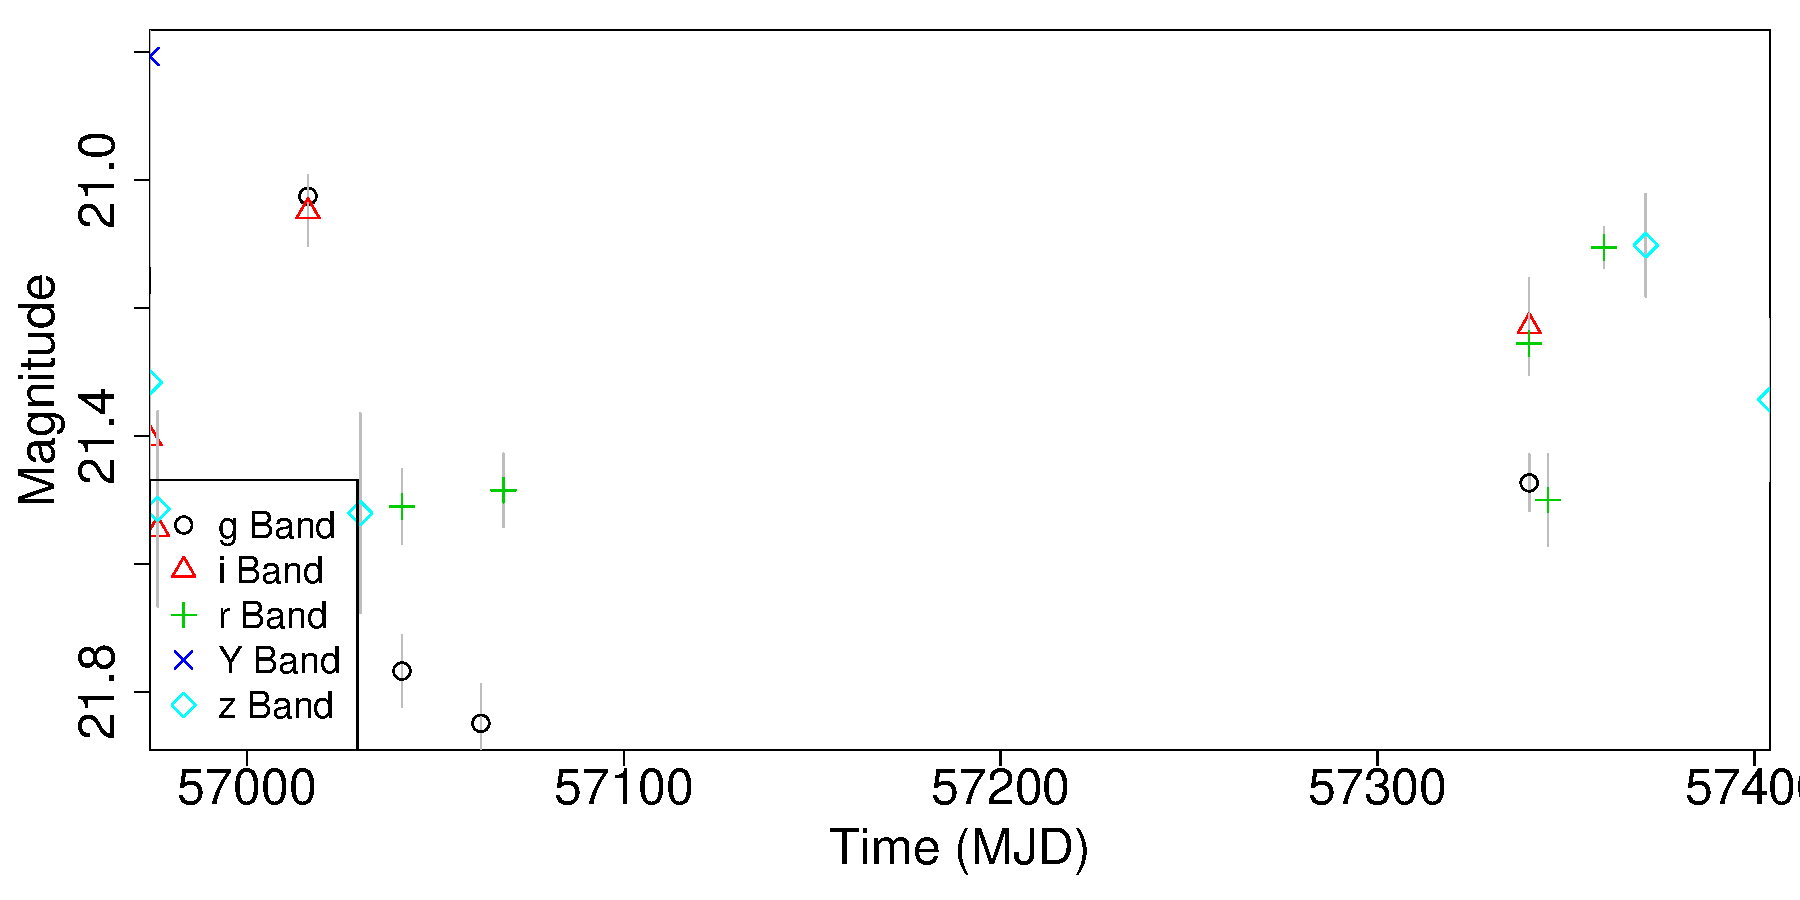
\includegraphics[scale=0.2]{figs/unfolded_des_2.pdf}
%% see one-class/des for code for des image

\vspace{.1in}

\begin{center}
  DES is \underline{deeper and wider} but \underline{sparsely sampled}.
\end{center}

\end{frame}



\section{Modeling and Classifying Variable Stars}

\subsection{Fourier Modeling of Light Curves}

\begin{frame}{Light Curve Notation}

  Data for star is $D=\{\{(t_{jb},m_{jb},\sigma_{jb})\}_{j=1}^{n_b}\}_{b=1}^B$
\begin{itemize}
\item $b=1,\ldots,B$ denotes band (ie filter)
\item $n_b$ is number of measurements in band $b$
\item $m_{jb}$ is brightness at time $t_{jb}$ with known uncertainty $\sigma_{jb}$
\end{itemize}

\begin{center}
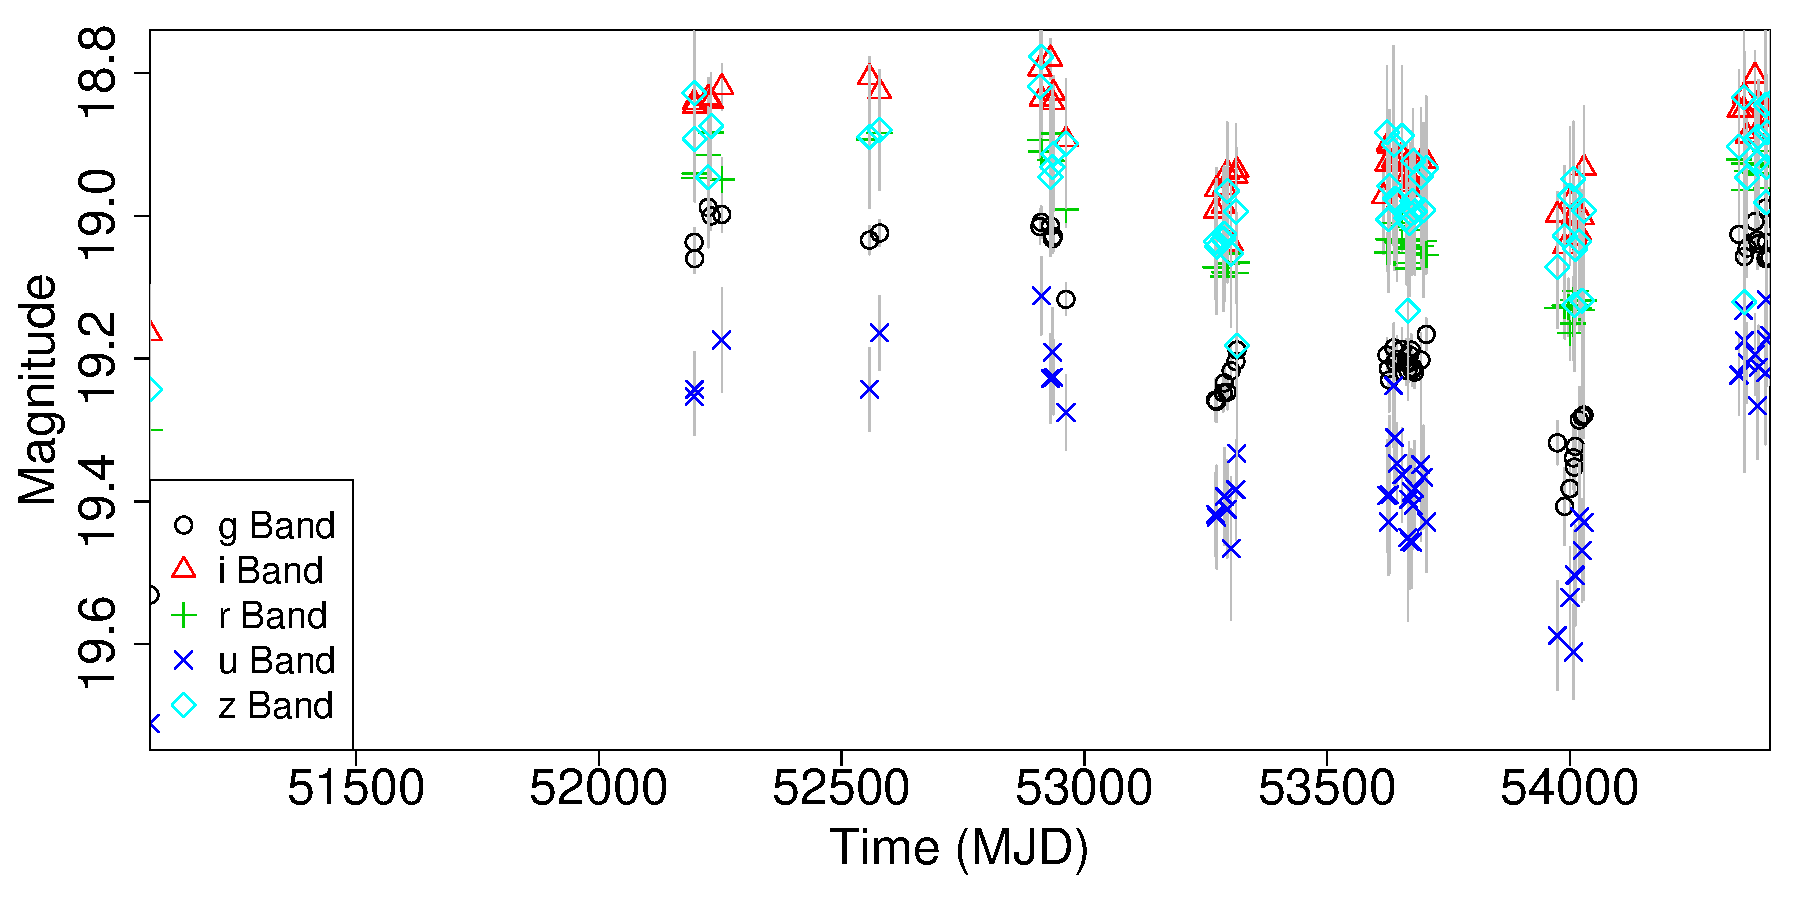
\includegraphics[scale=0.3]{figs/unfolded_7904669.pdf}
\end{center}

\begin{center}
  Heteroskedastic error with known variance.
\end{center}

\end{frame}

\begin{frame}{Fourier Period Estimation and Feature Extraction}

\textbf{Method:} Model light curve variation in each filter as sinusoid with $K$ harmonics. \cite{mondrik2015multiband,zechmeister2009generalised,lomb1976least,scargle1982studies,schwarzenberg1996fast}

\begin{equation*}
m_{jb} = \beta_b + \sum_{k=1}^K a_{bk}\sin(\omega t_{jb} + \phi_{bk}) + \epsilon_{jb}
\end{equation*}
where $\epsilon_{jb} \sim N(0,\sigma_{jb}^2)$.

\begin{itemize}
\item $(2K + 1)B + 1$ parameters. Pure sine $3B + 1$ parameters.
\item Maximum likelihood has closed form solution at fixed $\omega$
\begin{itemize}
\item Maximization strategy: Grid search on $\omega$.
\end{itemize}
\end{itemize}

\end{frame}


\begin{frame}{Example of Maximum Likelihood Fit with $K=2$}

\vspace{-.1in}

\begin{center}
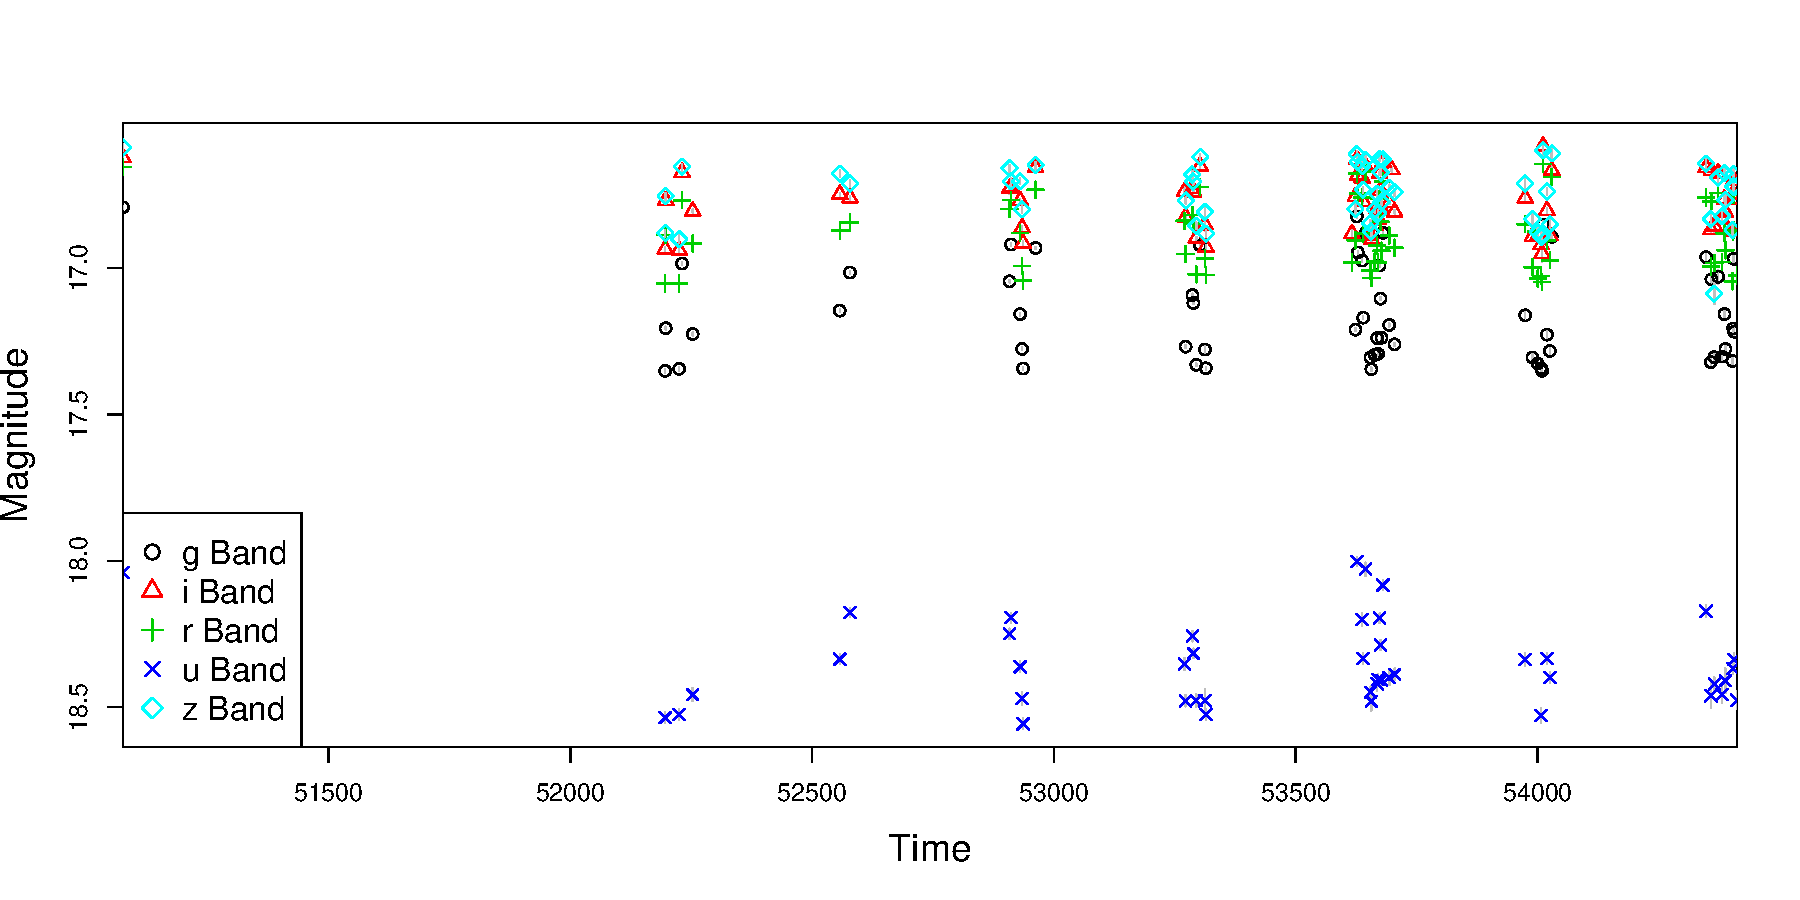
\includegraphics[scale=.25]{figs/rrlyrae_nomodel_fit.pdf}\\
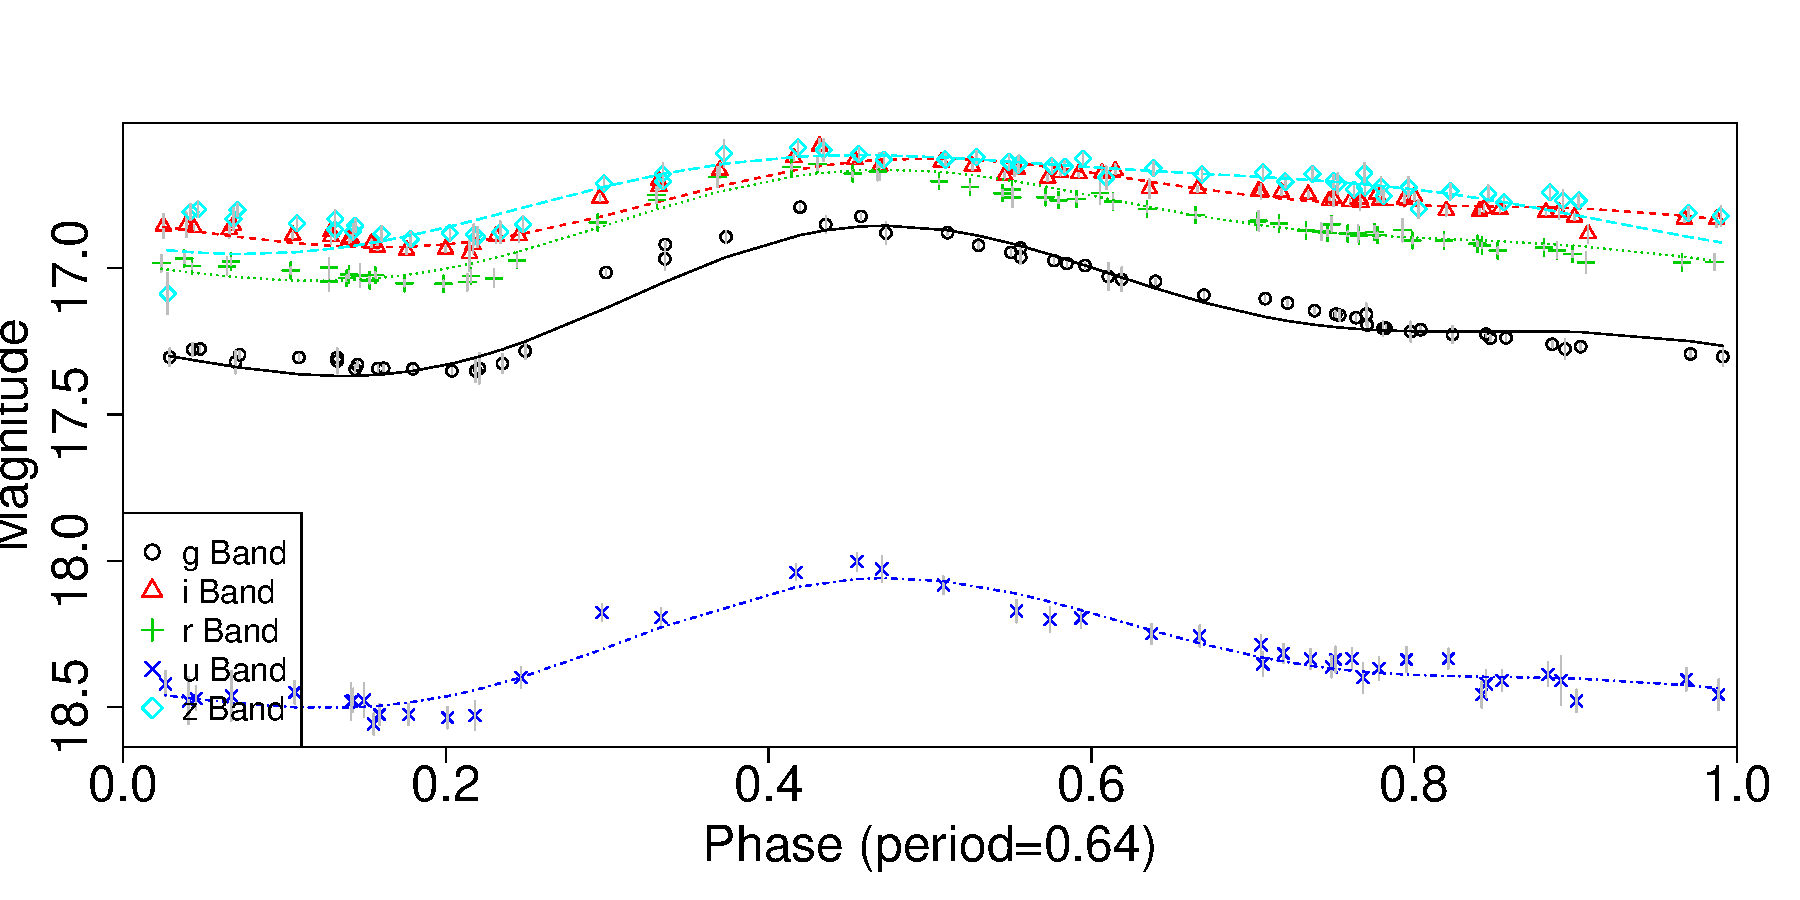
\includegraphics[scale=.25]{figs/rrlyrae_model_fit.pdf}\\
Total of $26$ parameters, model estimates period well.
\end{center}

\end{frame}

\begin{frame}{Model Output Used for Classification}

  \begin{center}
    Fit $K=2$ model to all 60,000 light curves. RRL separate well.
  \end{center}
  
\begin{center}
  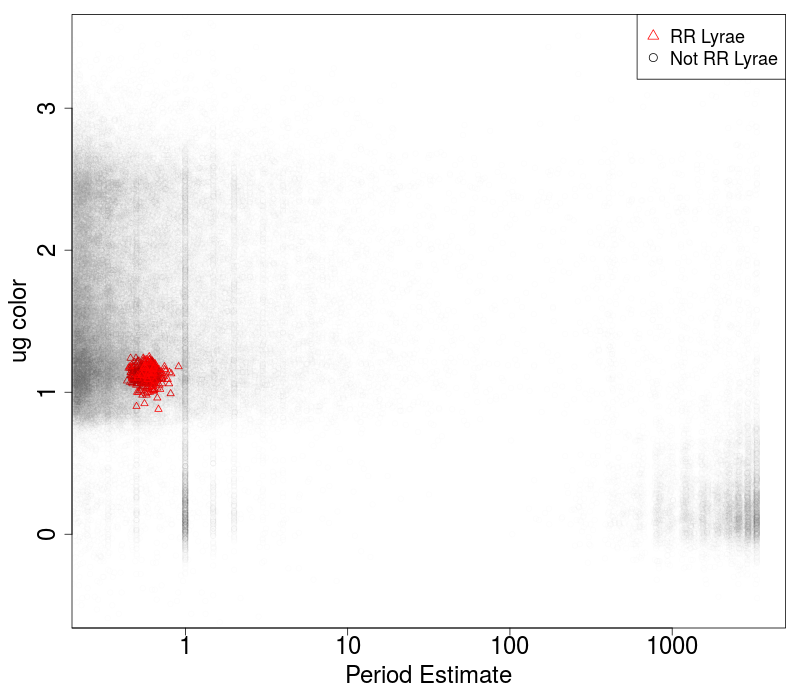
\includegraphics[scale=.2]{figs/sdss_color_period.png}
  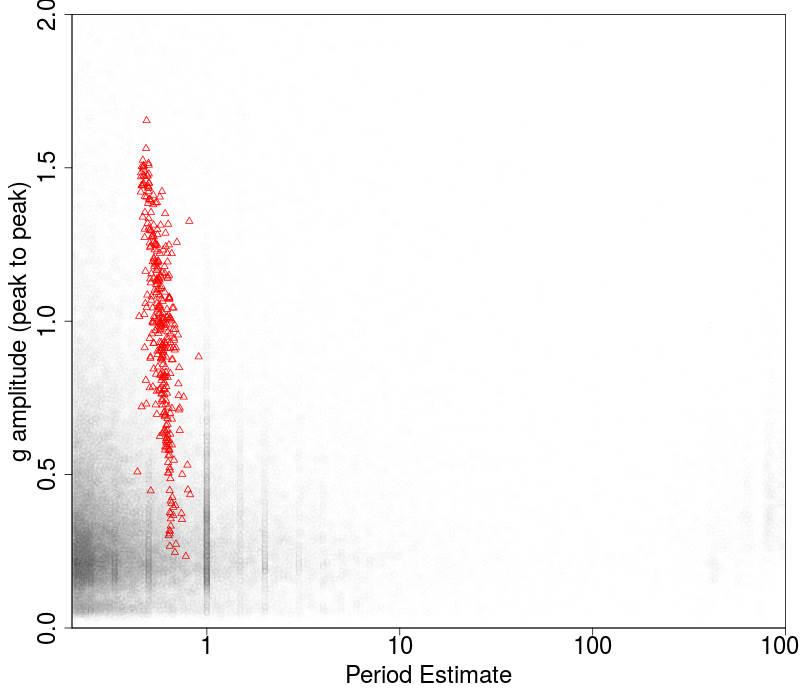
\includegraphics[scale=.2]{figs/sdss_gamp_period.png}
\end{center}


%%% TODO: make scatterplot of two features

\end{frame}


%% \begin{frame}{Challenge: DES Light Curves are Sparsely Sampled}


%% \begin{center}
%% 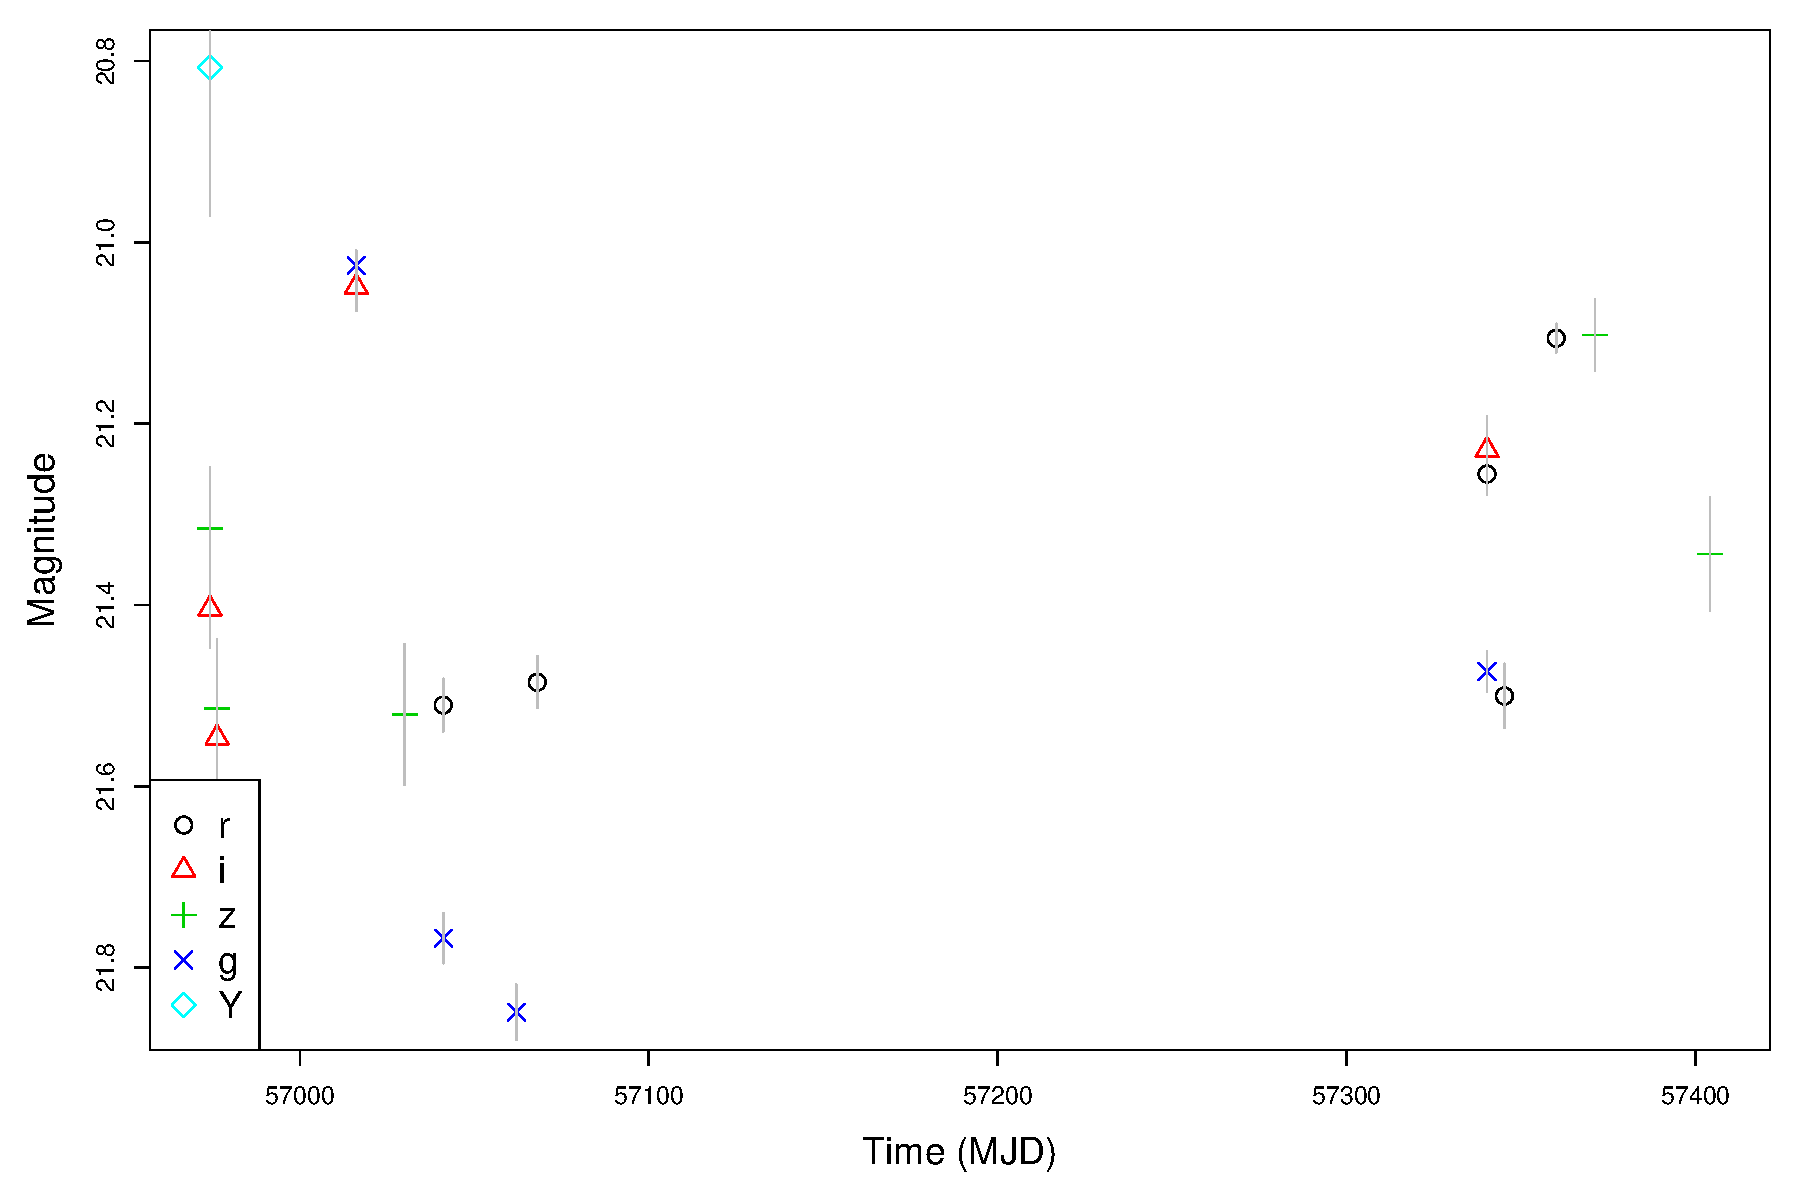
\includegraphics[scale=.3]{figs/des_2.pdf}
%% \end{center}

%% \vspace{-.2in}

%% \begin{center}
%% \small{Dark Energy Survey light curve. Period estimation, classification, and distance estimation difficult for this quality data.}
%% \end{center}

%% \end{frame}






%% \begin{frame}{Surveys Collecting Sparsely Sampled Light Curves}

%% \begin{itemize}
%% \item Dark Energy Survey (DES)
%% \begin{itemize}
%% \item 10 photometric measurements in ($g$,$i$,$r$,$z$,$Y$) over five years
%% \item depths to 24 mag in $i$
%% \item $\approx$ 100 million stars
%% \end{itemize}
%% \item Pan--STARRS
%% \end{itemize}
%% \end{frame}



%%%%%%%%
%%%%%%%% TODO: introduce model, discuss fitting
%%%%%%%%

\begin{frame}{Applying Methodology to DES Data}
  DES will collect $\approx$ 50 observations for each star.

  \begin{itemize}
    \item \textbf{Strategy 1:} Fourier feature extraction with $K=1$ harmonic (16 parameters). \underline{Problem:} This simple model is misspecified.

  \begin{center}
    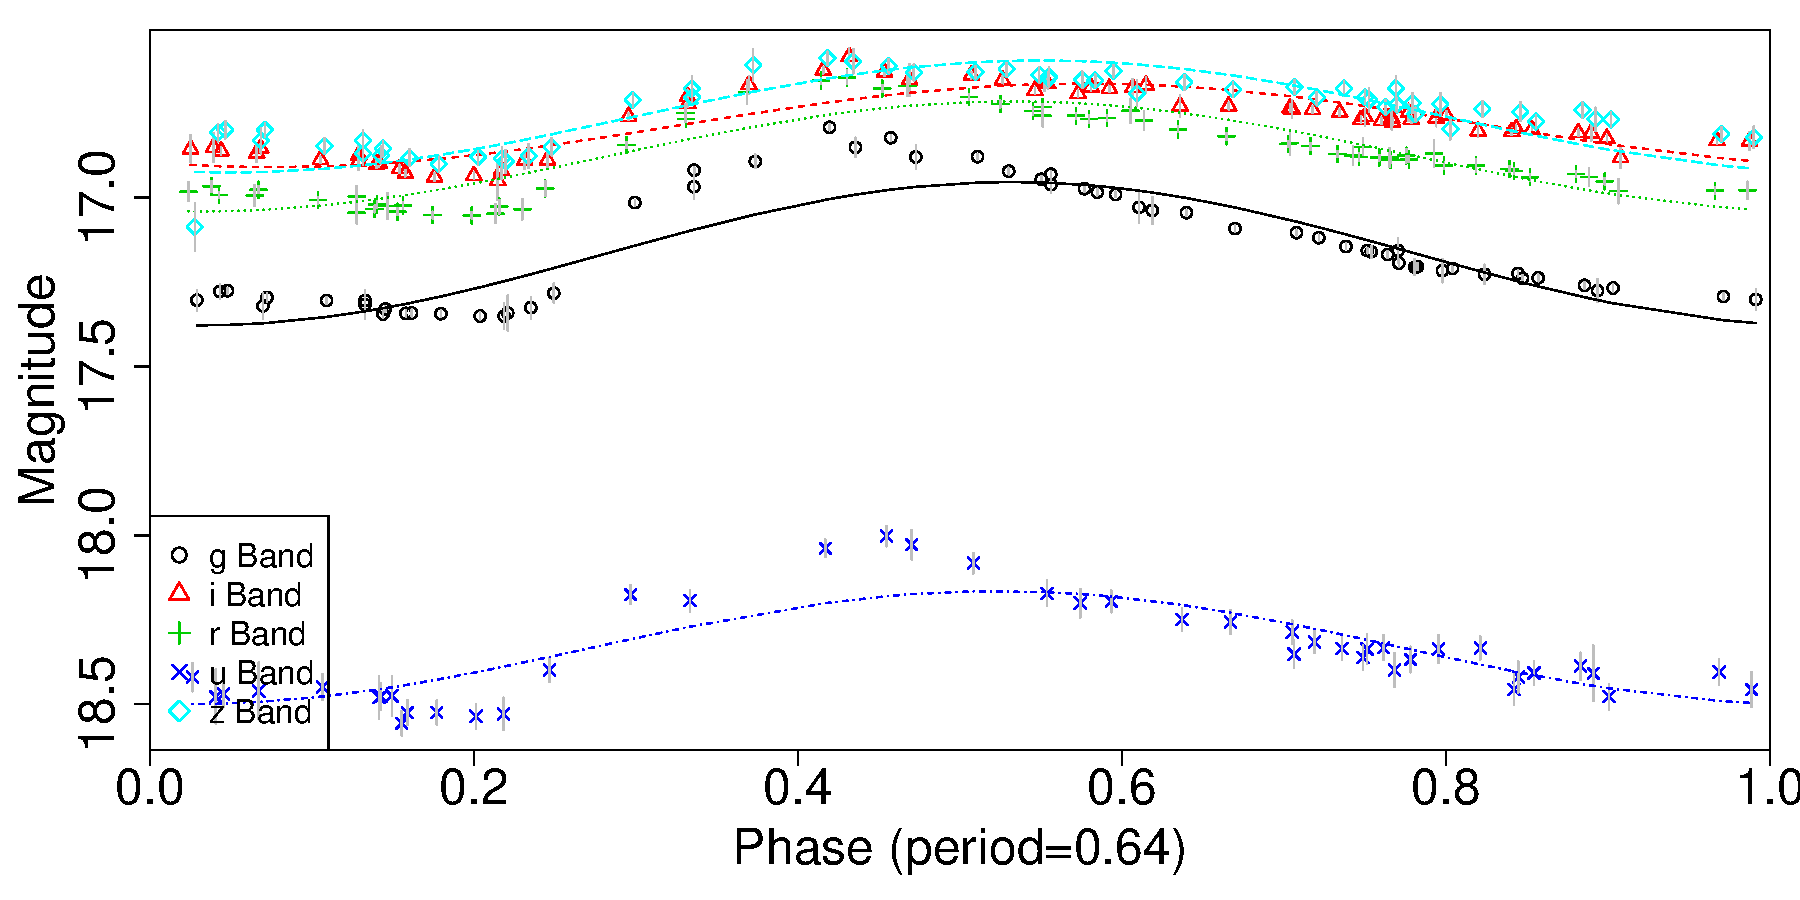
\includegraphics[scale=.25]{figs/rrlyrae_model_fit_sine.pdf}
  \end{center}

\item \textbf{Strategy 2:} Fourier feature extraction with $K>1$ harmonics. With $K=2$, 26 parameters and 50 data points. \underline{Problem:} Large variance in parameter estimates.
  \end{itemize}
  %% put best sampled star here
\end{frame}


\begin{frame}{Outline of Methodology}

\underline{Fitting Approximate Models with Heteroskedastic Errors}\\
\begin{itemize}
\item Define what approximate / misspecified model is estimating.
\item With heteroskedasticity, optimal weighting no longer $\sigma^{-2}$.
\item Construct adaptive estimator for optimal weight.
\end{itemize}


\vspace{.2in}

\underline{Improved Model for RR Lyrae Stars}
\begin{itemize}
\item Build parsimonious (few free parameters) RRL model.
\item Assess model accuracy on SDSS Stripe 82 RRL.
\end{itemize}

\end{frame}




\subsection{Fitting Approximate Models with Heteroskedastic Errors}

\begin{frame}{Approximate Models with Heteroskedastic Error}

  Sine model MLE for period:
  \begin{equation*}
    \widehat{\omega} = \argmin{\omega} \min_{\V{a},\V{\beta},\V{\phi}} \sum_{b=1}^B \sum_{j=1}^{n_b} \left(\frac{m_{bj} - \beta_{b} - a_b\sin(\omega t_{bj} + \phi_b)}{\sigma_{bj}}\right)^2
  \end{equation*}
  
  
  

  \textbf{Questions:}
  \begin{itemize}
  \item Is period of best fitting sine function converging to true period of function?\\
  \item Does weighting observations by inverse of the variance make sense when model is an approximation?
  \end{itemize}
  
\end{frame}

\begin{frame}{Simple Case: Linear Regression and WLS}
\begin{itemize}
\item Observe $\{(y_i,x_i,\sigma_i)\}_{i=1}^n$ i.i.d. where
  \begin{equation*}
    y_i = f(x_i) + \sigma_i\epsilon_i 
  \end{equation*}
  where $\E[\epsilon_i] = 0$  and $\Var(\epsilon_i) = 1$
\item Weighted least squares (WLS) estimator is
  \begin{equation*}
    \widehat{\beta}(W) = (X^TWX)^{-1}X^TWY
  \end{equation*}
  where
  \begin{itemize}
    \item $W$ is diagonal weight matrix
    \item $Y = (y_1,\ldots,y_n)^T$ is response
    \item $X = (x_1^T,\ldots,x_n^T)^T$ is design
  \end{itemize}
\end{itemize}

\begin{center}
\textbf{If $f(x) = x^T\beta$ then $\widehat{\beta}(\Sigma^{-1})$ is best linear unbiased.\\ ($\Sigma$ diagonal, $\Sigma_{ii} = \sigma_i^2$)}
\end{center}
\end{frame}

\begin{frame}{What are we estimating?}
Define the ``true'' $\beta$ as the best linear approximation to $f$ i.e.
  \begin{equation*}
  \beta \equiv \argmin{\beta} \E[(f(x) - x^T\beta)^2] = \E[xx^T]^{-1}\E[xf(x)]
\end{equation*}
  %% $\beta^T x$ is optimal MSE predictor among linear functions of $x$:
  %% \begin{equation*}
  %%   \beta = \argmin{\beta} \E[(y - x^T\beta)^2]
  %% \end{equation*}

Example:

\vspace{-.2in}

\begin{center}
        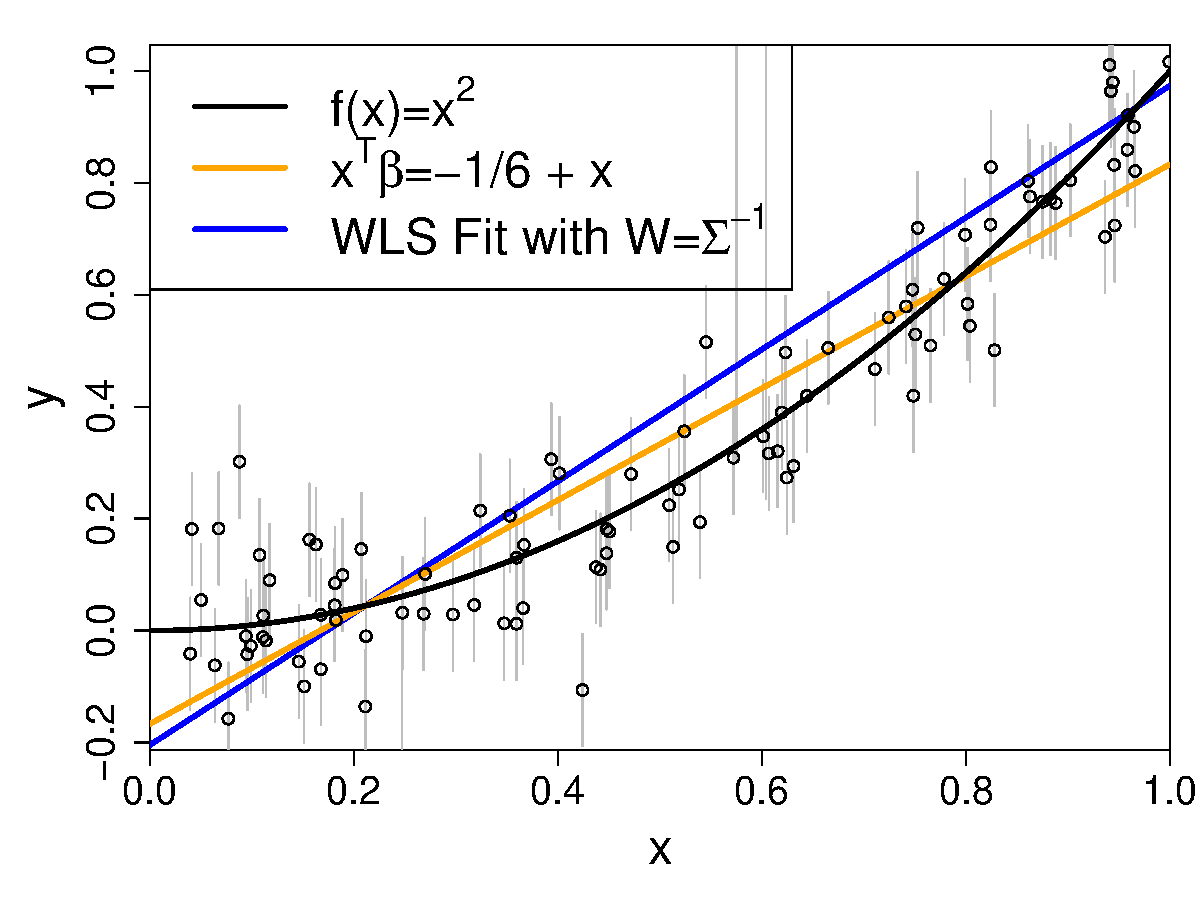
\includegraphics[scale=0.4]{figs/data.pdf}
  \end{center}


  %% \begin{columns}
  %%   \begin{column}{0.5\textwidth}
  %%     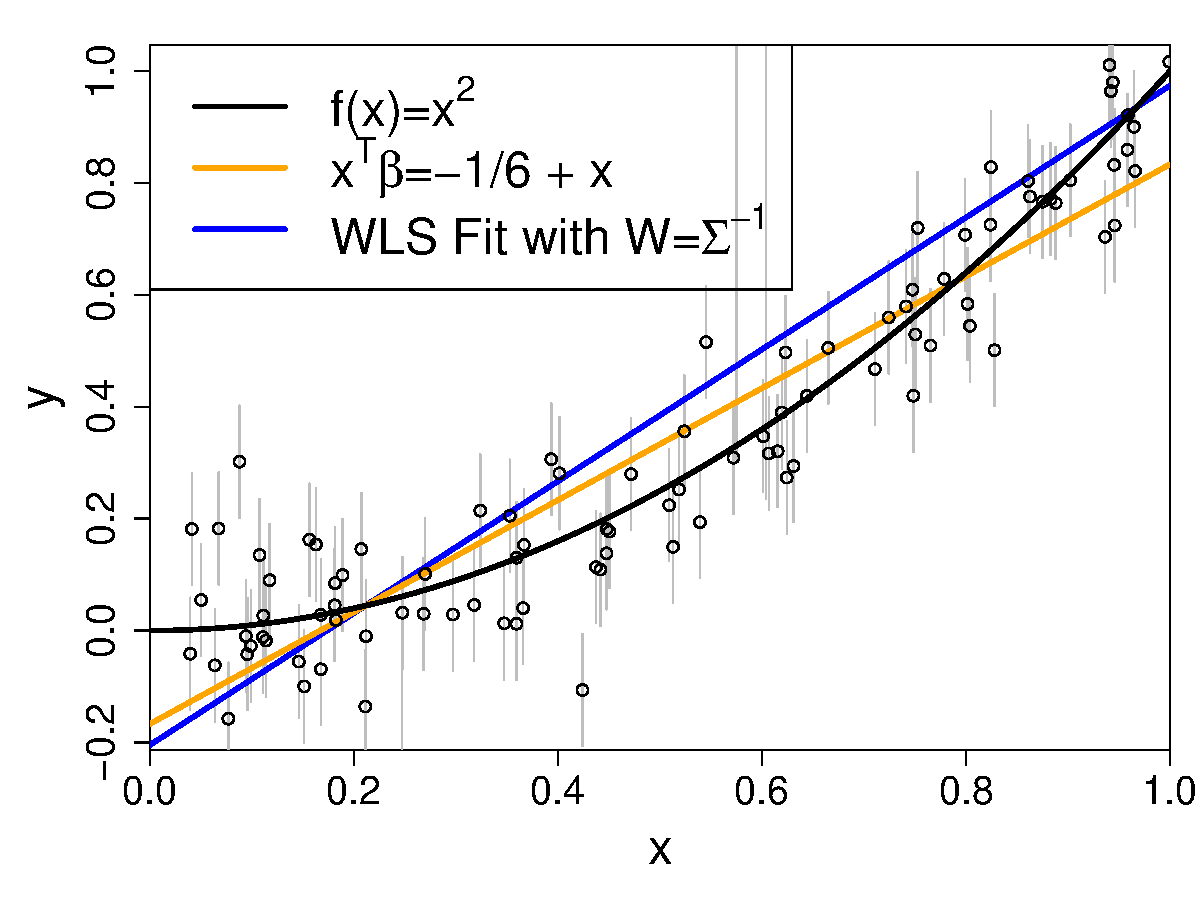
\includegraphics[scale=0.3]{figs/data.pdf}
  %%   \end{column}
  %%   \begin{column}{0.5\textwidth}
  %%     \begin{align*}
  %%       &x_i \sim Unif[0,1]\\
  %%       &\sigma_i \sim f_{\sigma}(\sigma) = \left\{
  %%         \begin{array}{lr}
  %%           0.05 \! &:  \! \sigma=0.01,1.0\\ 
  %%           0.9  \! &: \! \sigma=0.1\\
  %%         \end{array} \right.\\
  %%       &y_i = x_i^2 + \epsilon_i
  %%       \end{align*}
  %%   \end{column}
  %% \end{columns}
\end{frame}

\begin{frame}{Weight Matrix}

  \begin{assumptions}[Weight Matrix]
  Consider diagonal, positive definite weight matrices
  \begin{equation*}
    \widehat{W}_{ii} = w(\sigma_i) +
  \end{equation*}
  where $w(\cdot)$ is some function.
  \end{assumptions}

  \vspace{.2in}
  
  \textbf{Important Cases:}
  \begin{itemize}
  \item $\widehat{W}_{ii} = w(\sigma_{i}) = 1$ (OLS)
  \item $\widehat{W}_{ii} = w(\sigma_{i}) = \sigma_{i}^{-2}$ (``Standard'' WLS)
  \item $\widehat{W}_{ii} = w(\sigma_{i}) = (\sigma_{i}^{2} + c)^{-1}$ (for some constant $c$)
  \end{itemize}
\end{frame}

\begin{frame}{Asymptotic Variance}

  \vspace{-.05in}
  
  \begin{theorem}
    Under regularity conditions, $x_i \, \indep \, \sigma_i$, and Weight Matrix Assumptions,
  \begin{equation*}
    \sqrt{n}(\widehat{\beta}(\widehat{W}) - \beta) \rightarrowd N(0,\nu(w))
  \end{equation*}
  where $g(x) = f(x) - x^T\beta$ and
  \begin{equation*}
    \nu(w) = \frac{\E[w^2]\overbrace{\E[xx^T]^{-1}\E[g^2(x)xx^T]\E[xx^T]^{-1}}^{\equiv A} + \E[\sigma^2w^2]\overbrace{\E[xx^T]^{-1}}^{\equiv B}}{\E[w]^2}.
  \end{equation*}
  \end{theorem}

  \vspace{-.05in}
  
  \textbf{Special Case:}
   If model is linear $g(x)=0$ and
    \begin{equation*}
      \nu(w) = \frac{\E[\sigma^2w^2]\E[xx^T]^{-1}}{\E[w]^2},
    \end{equation*}
   which is minimized by $w(\sigma) = \sigma^{-2}$.
  
\end{frame}

\begin{frame}{Optimal Weight Matrix}

  Consider linear function
  \begin{equation*}
    \Gamma: \mathbb{R}^p \times \mathbb{R}^p \rightarrow \mathbb{R}
  \end{equation*}
  such that $\Gamma(C) > 0$ for all $C$ positive definite.
  
  \begin{theorem}[Optimal Weighting]
    \begin{equation*}
      w(\sigma) = \argmin{w} \Gamma(\nu(w)) = \frac{1}{\sigma^2 + \Gamma(A)\Gamma(B)^{-1}}
    \end{equation*}
  \end{theorem}

  \begin{theorem}[Adaptivity]
    Under regularity conditions, 
  \end{theorem}

  %% \begin{itemize}
  %% \item $\Gamma(A)\Gamma(B)^{-1}$ reduces influence of low variance observations.
  %% \end{itemize}

\end{frame}

\begin{frame}{Small Simulation}

\end{frame}

%% \begin{frame}{Back to Variable Stars}

%% \end{frame}

%% \begin{frame}{Simulated Results on Variable Stars}

%% \begin{table}[ht]
\centering
\begin{tabular}{c|cc|cc|cc}
 &   $K=1$ &    & $K=2$ &    & $K=3$ &  \\ 
  \hline
n & $\Sigma^{-1}$ &  $I$ & $\Sigma^{-1}$ &  $I$ & $\Sigma^{-1}$ &  $I$ \\
  \hline10&0.09&0.16&0.13&0.11&0.03&0.03\\20&0.46&0.58&0.63&0.68&0.69&0.77\\30&0.64&0.78&0.71&0.82&0.82&0.86\\40&0.75&0.79&0.80&0.85&0.87&0.92\\\hline
\end{tabular}
\caption{Fraction of periods estimated correctly (within 1\%) using models with $K=1,2,3$ harmonics ($p=4,5,8$ parameters, respectively). Ignoring the observation uncertainties ($I$) in the fitting is superior to using them ($\Sigma^{-1}$). The standard deviation on these accuracies is no larger than $\sqrt{0.5(1-0.5)/238} \approx 0.032$ .}
\label{tab:period_est_results}
\end{table}

  
%% \end{frame}


\begin{frame}{Application to Variable Star Period Estimation}
\begin{itemize}
\item 238 SDSS Stripe 82 (g--band data only)
\item Downsample light curves to 10, 20, 30, and 40 observations.

\def \tw {.15}
  
  %%\begin{textblock*}{3cm}(1cm,3.1cm) % {block width} (coords)
%% \begin{center}
%% 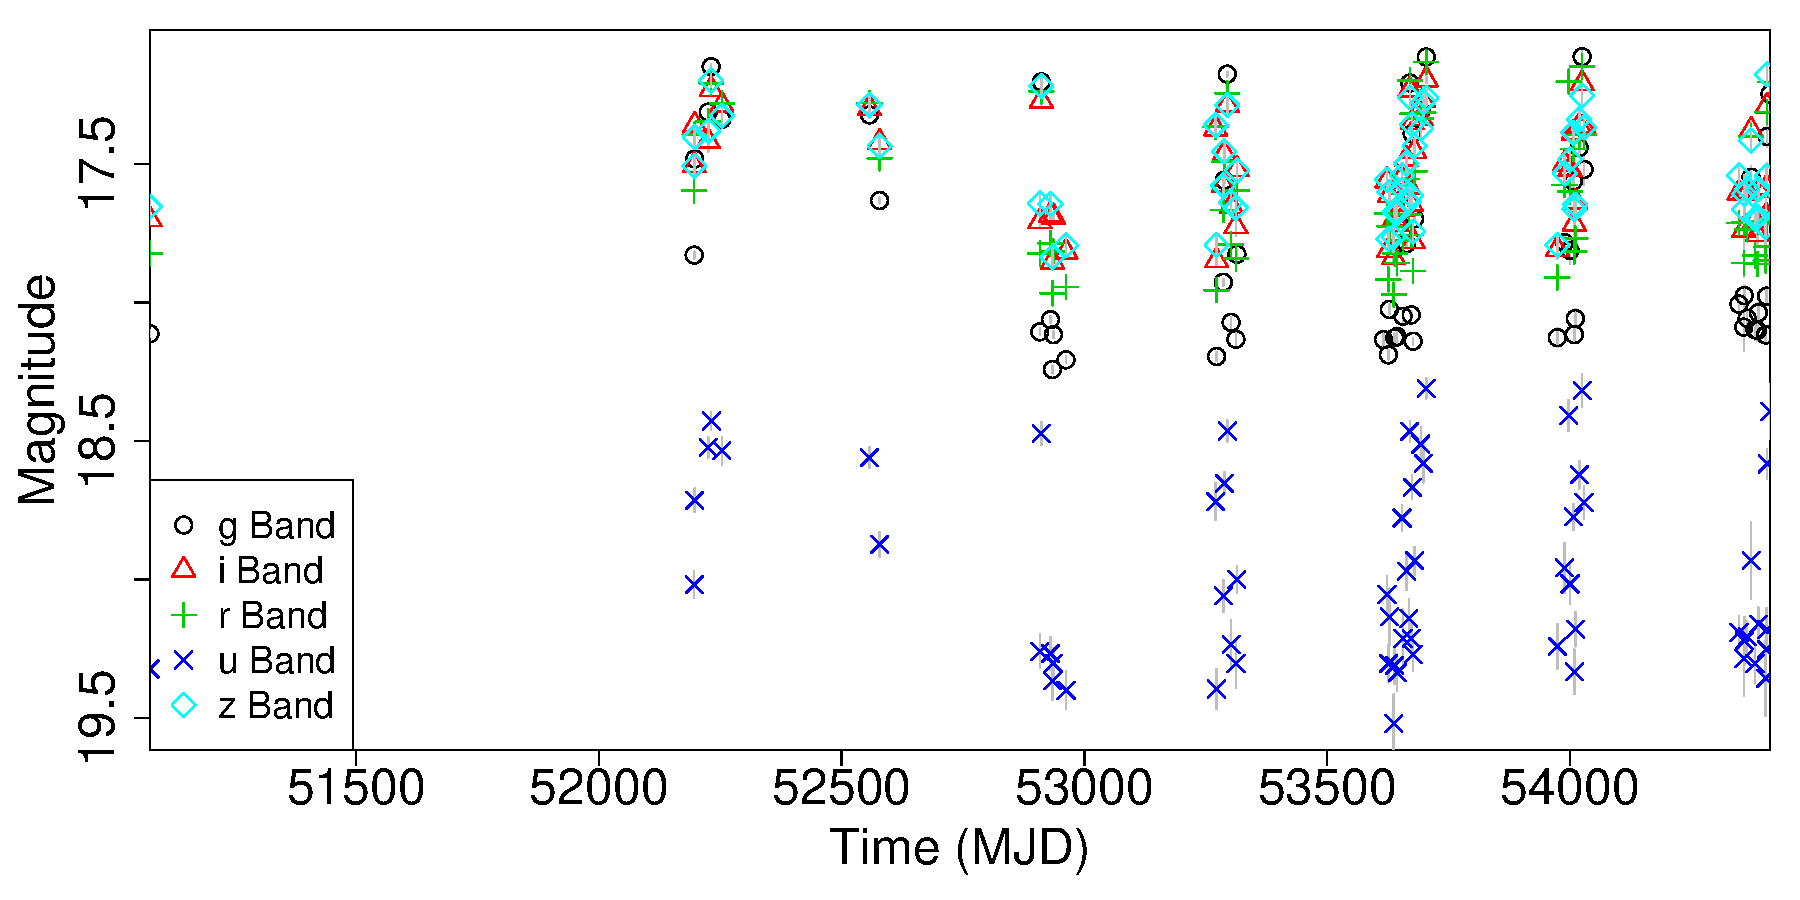
\includegraphics[scale=\tw]{figs/unfolded_13350.pdf}
%% 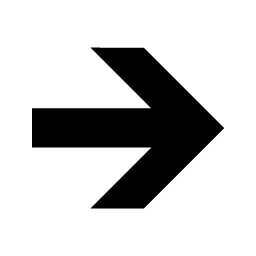
\includegraphics[scale=\tw]{figs/rightarrow.png}
%% 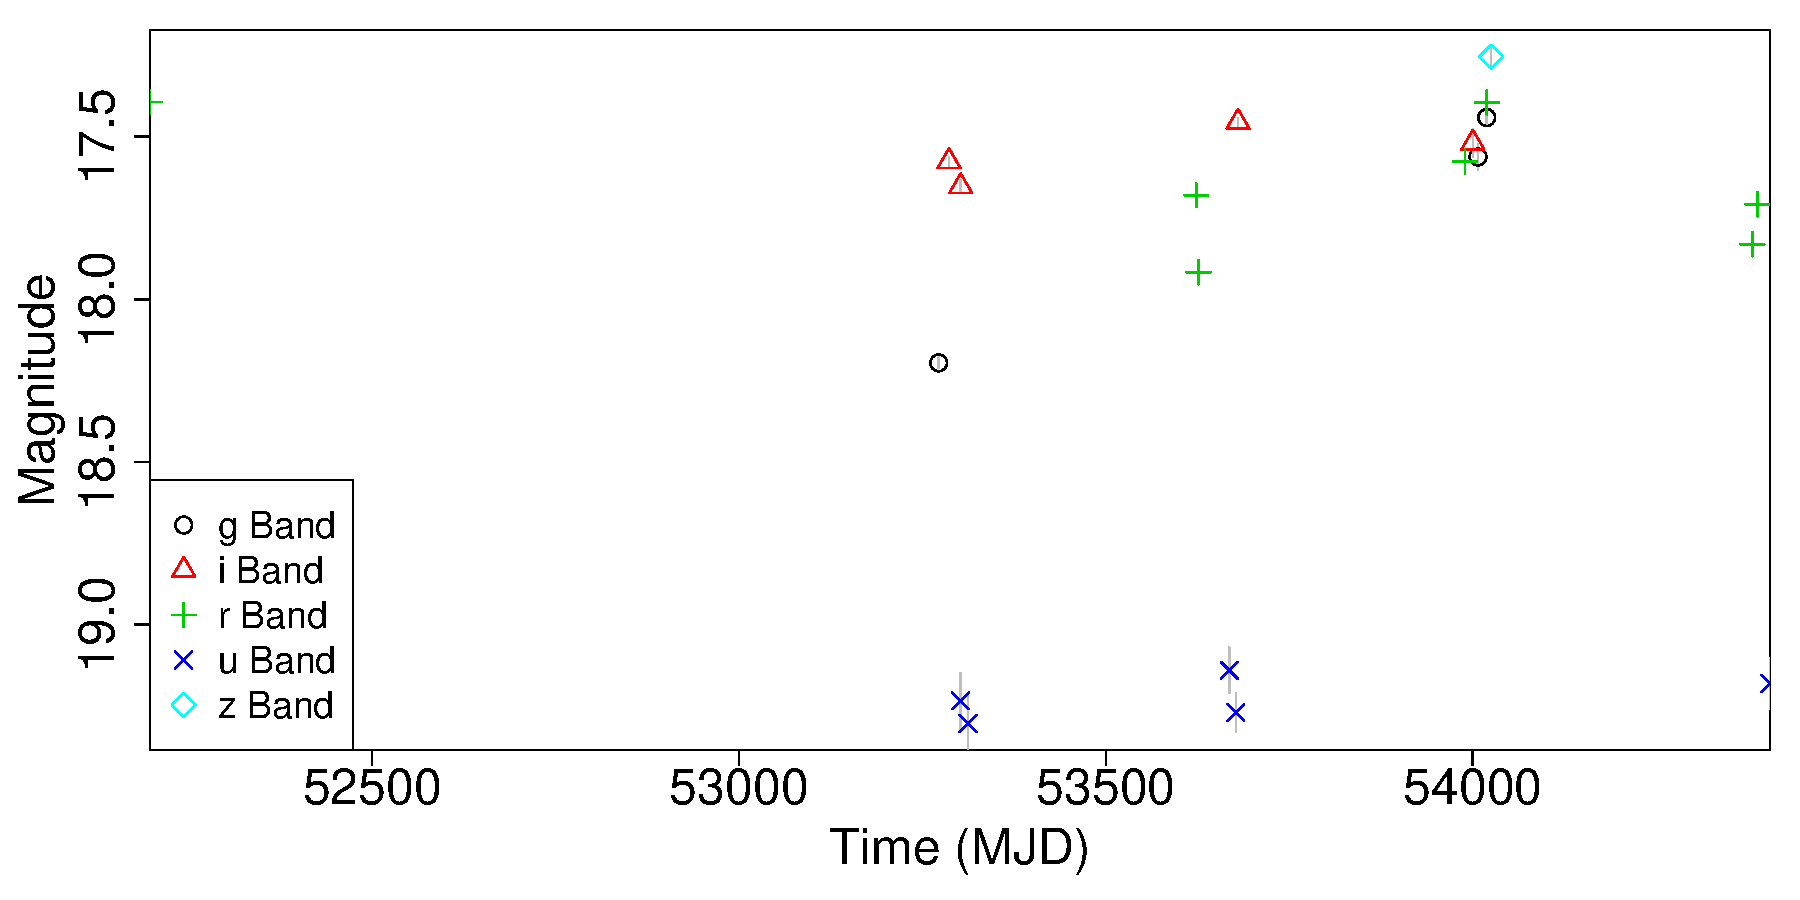
\includegraphics[scale=\tw]{figs/unfolded_13350down.pdf}
%% \end{center}


%% \begin{figure}[center]
%% 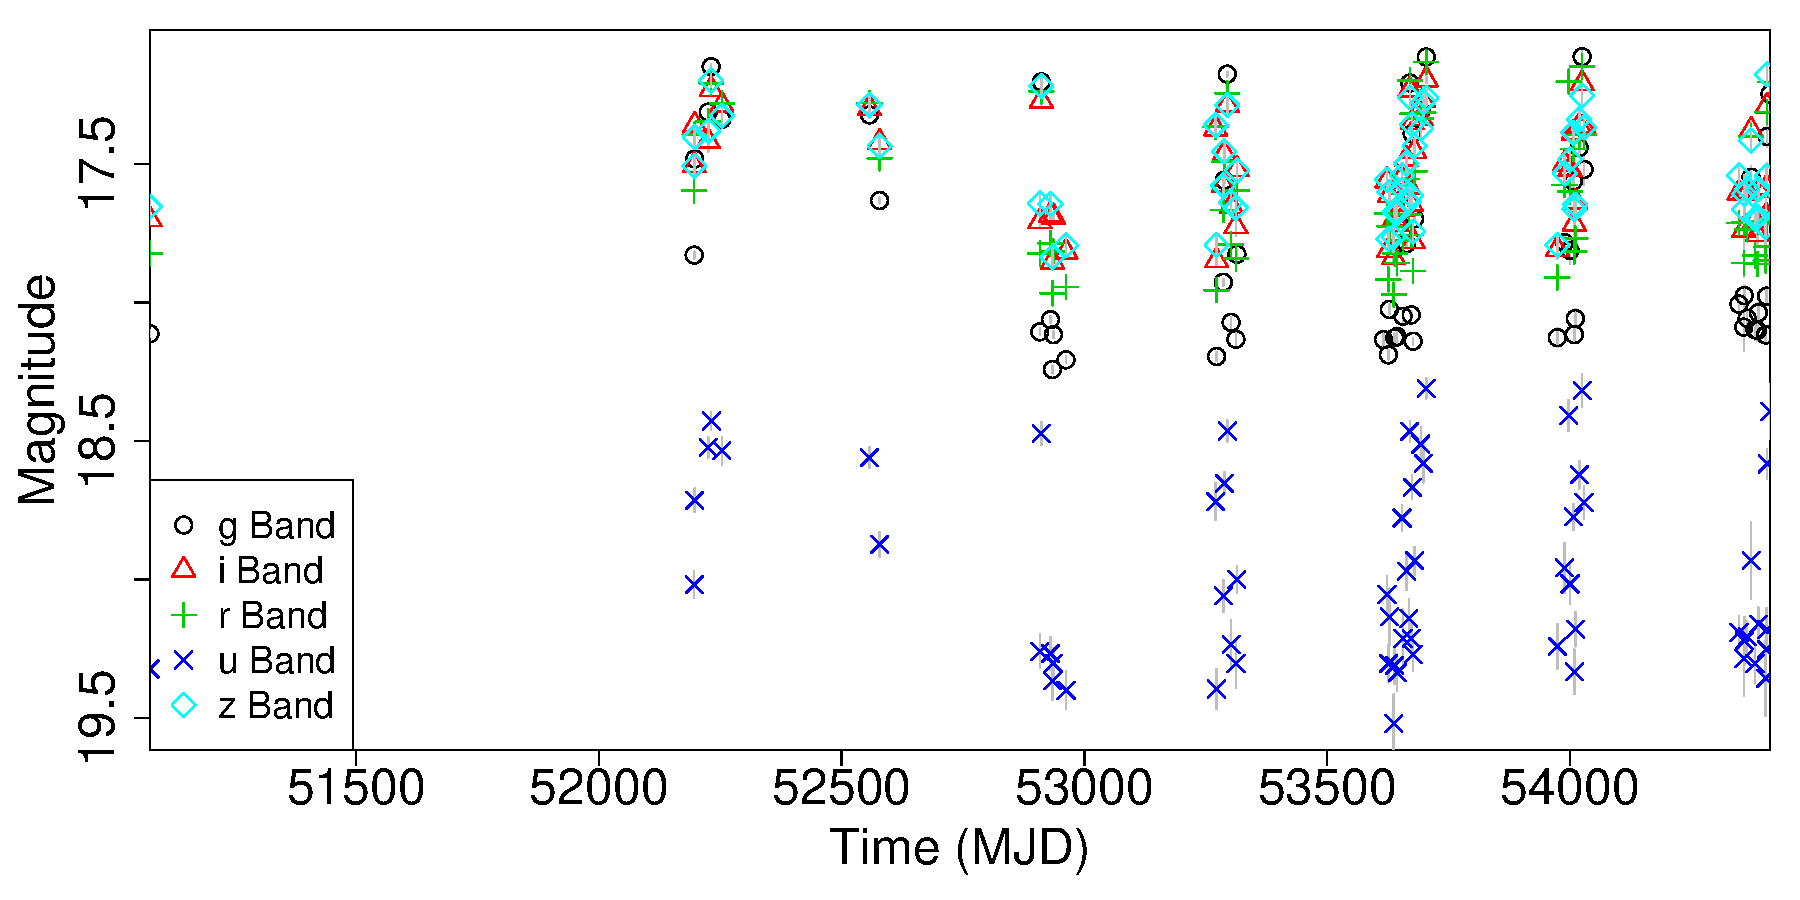
\includegraphics[scale=\tw]{figs/unfolded_13350.pdf}
%% 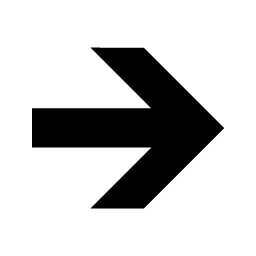
\includegraphics[scale=\tw]{figs/rightarrow.png}
%% 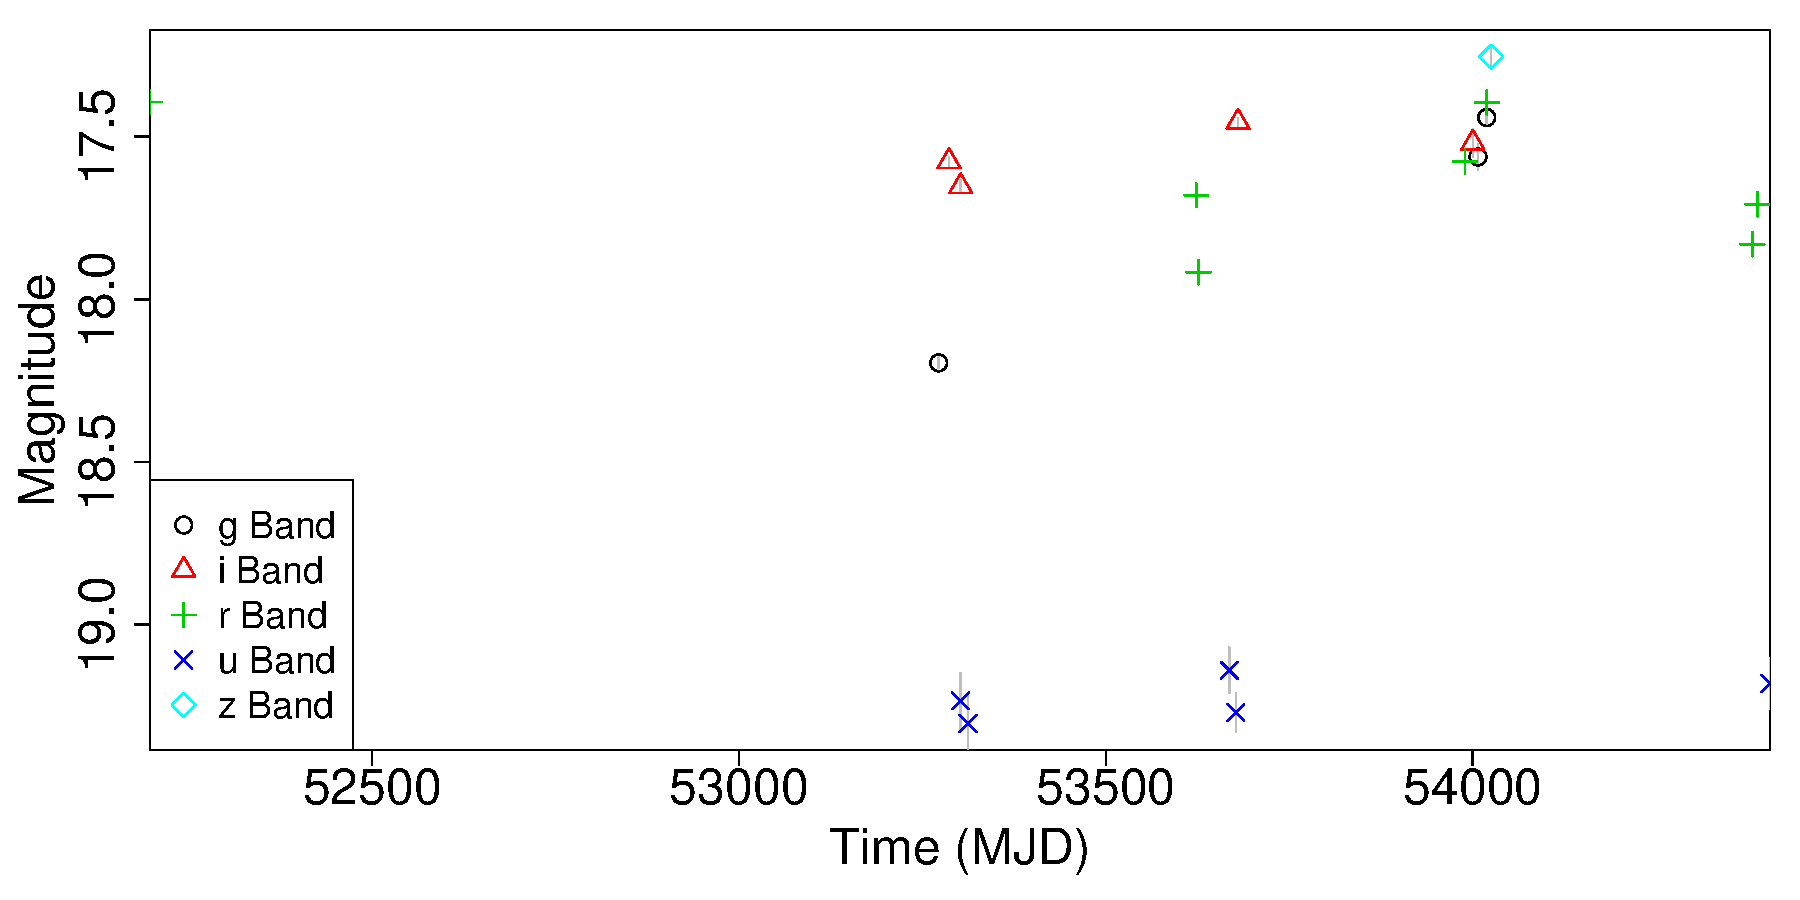
\includegraphics[scale=\tw]{figs/unfolded_13350down.pdf}
%% \end{figure}

\begin{minipage}{6in}
  \raisebox{-0.5\height}{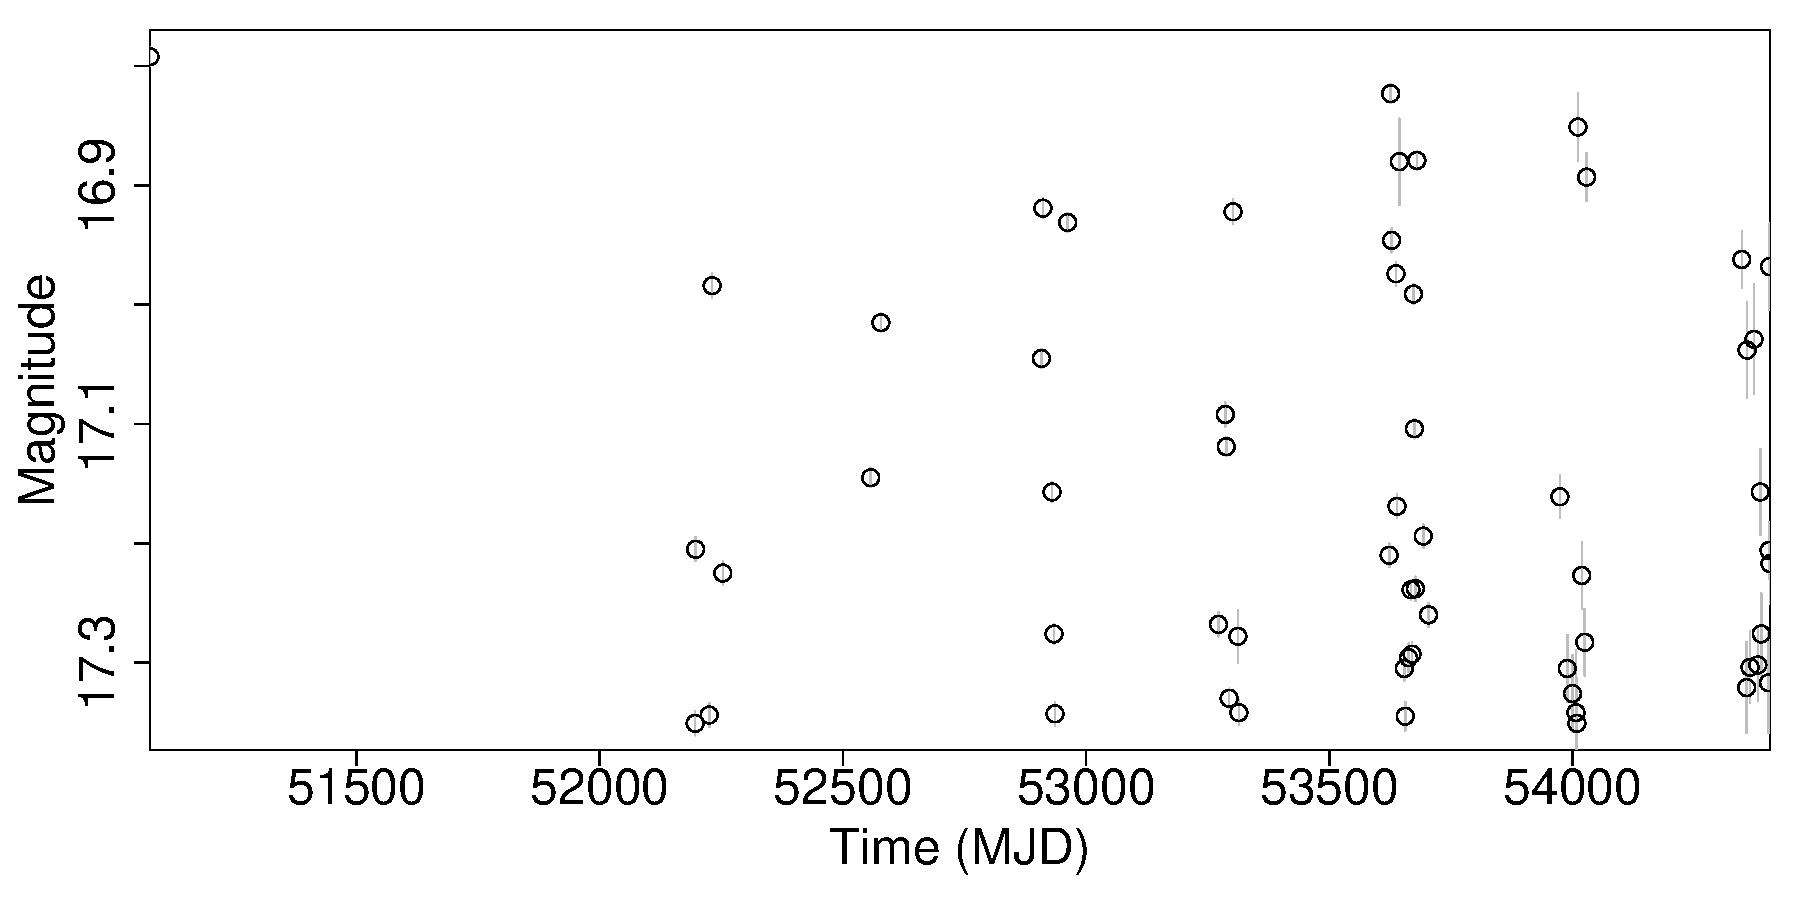
\includegraphics[scale=\tw]{figs/unfolded_4099_g.pdf}}
  \raisebox{-0.5\height}{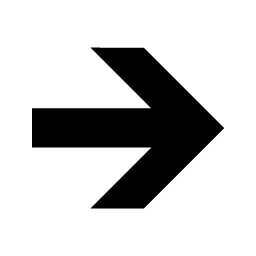
\includegraphics[scale=\tw]{figs/rightarrow.png}}
  \raisebox{-0.5\height}{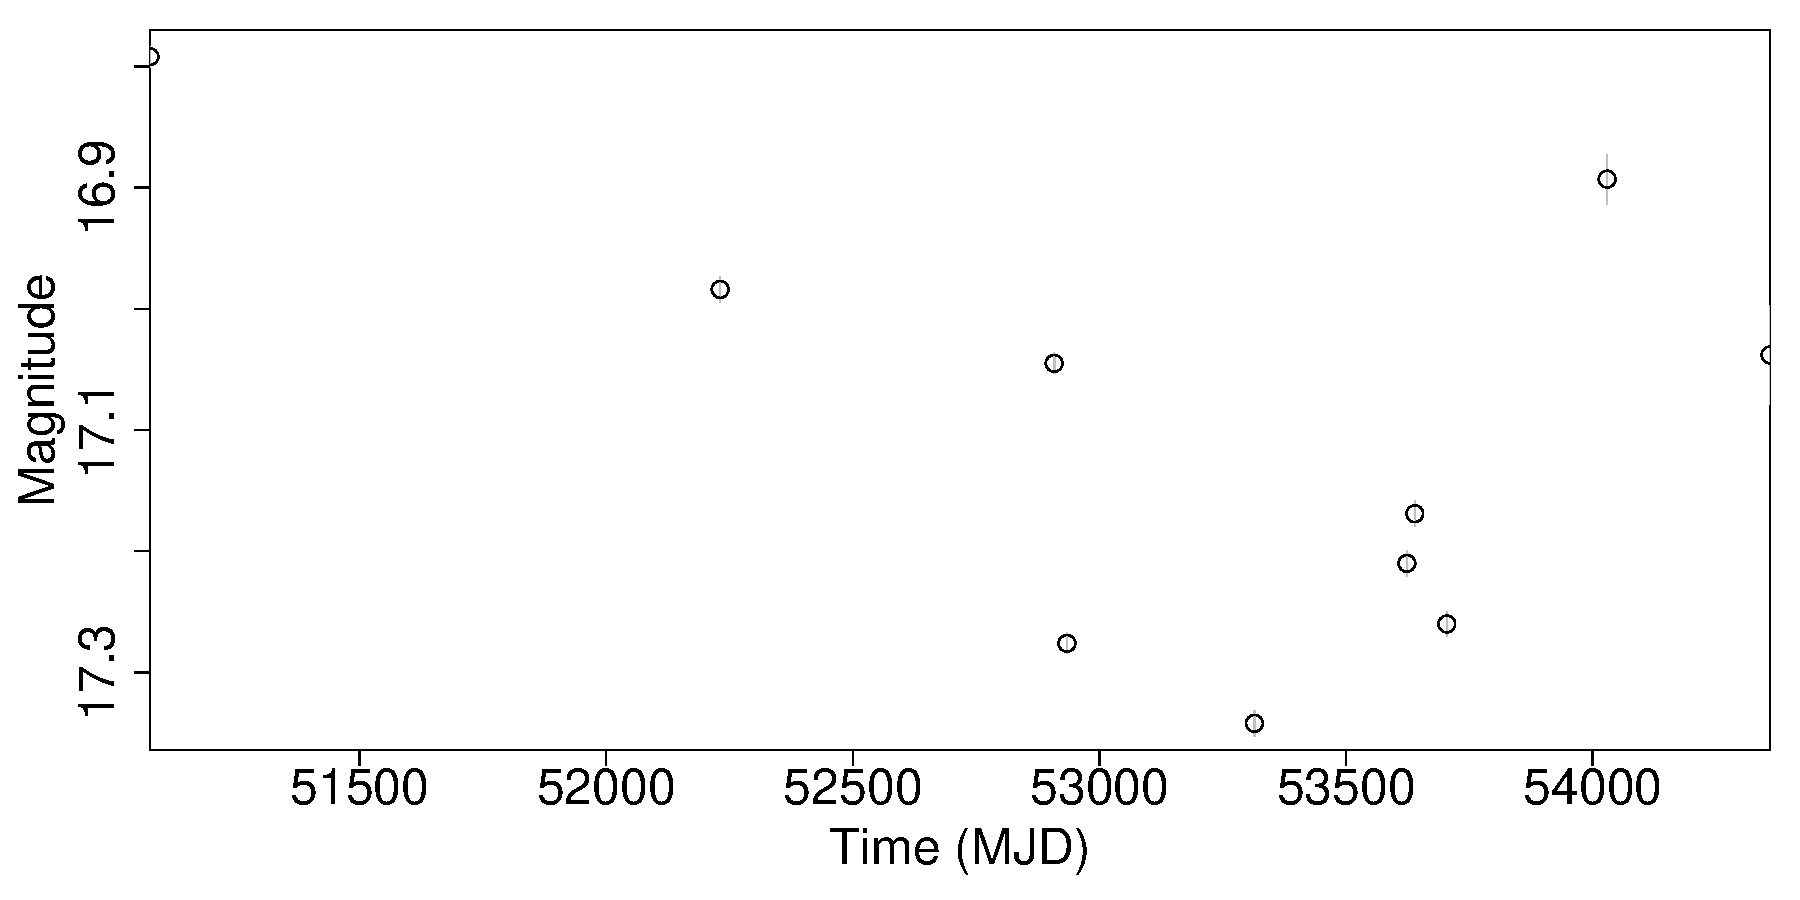
\includegraphics[scale=\tw]{figs/unfolded_4099_g_down.pdf}}
\end{minipage}

%%\end{textblock*}


%%  \begin{textblock*}{3cm}(5.5cm,3.5cm) % {block width} (coords)

%%\end{textblock*}

%%  \begin{textblock*}{3cm}(6.75cm,3.1cm) % {block width} (coords)

%%\end{textblock*}
  
\item Compare
  \begin{equation*}
    \widehat{\omega}(\Sigma^{-1}) = \argmin{\omega} \min_{a,\beta,\phi} \sum_{j=1}^{n} \left(\frac{m_{j} - \beta - a\sin(\omega t_{j} + \phi)}{\sigma_{j}}\right)^2
  \end{equation*}

  \begin{equation*}
    \widehat{\omega}(I) = \argmin{\omega} \min_{a,\beta,\phi} \sum_{j=1}^{n} \left(m_{j} - \beta - a\sin(\omega t_{j} + \phi)\right)^2
  \end{equation*}

  
  
  
\end{itemize}
\end{frame}


\begin{frame}{Results}

\begin{table}[ht]
\centering
\begin{tabular}{c|cc|cc|cc}
 &   $K=1$ &    & $K=2$ &    & $K=3$ &  \\ 
  \hline
n & $\Sigma^{-1}$ &  $I$ & $\Sigma^{-1}$ &  $I$ & $\Sigma^{-1}$ &  $I$ \\
  \hline10&0.09&0.16&0.13&0.11&0.03&0.03\\20&0.46&0.58&0.63&0.68&0.69&0.77\\30&0.64&0.78&0.71&0.82&0.82&0.86\\40&0.75&0.79&0.80&0.85&0.87&0.92\\\hline
\end{tabular}
\caption{Fraction of periods estimated correctly (within 1\%) using models with $K=1,2,3$ harmonics ($p=4,5,8$ parameters, respectively). Ignoring the observation uncertainties ($I$) in the fitting is superior to using them ($\Sigma^{-1}$). The standard deviation on these accuracies is no larger than $\sqrt{0.5(1-0.5)/238} \approx 0.032$ .}
\label{tab:period_est_results}
\end{table}


%% \vspace{.1in}
%% \textbf{Conclusion:} Not using the photometric errors is better than using them because the sinusoidal model is misspecified.
\end{frame}


\begin{frame}{Conclusions}

\end{frame}




\subsection{Improved Model for RR Lyrae Stars}

\begin{frame}{Building a Better Model}

\end{frame}

\begin{frame}{Parsimonious RR Lyrae Model}


\begin{center}
global parameters fit once for all RR Lyrae\\
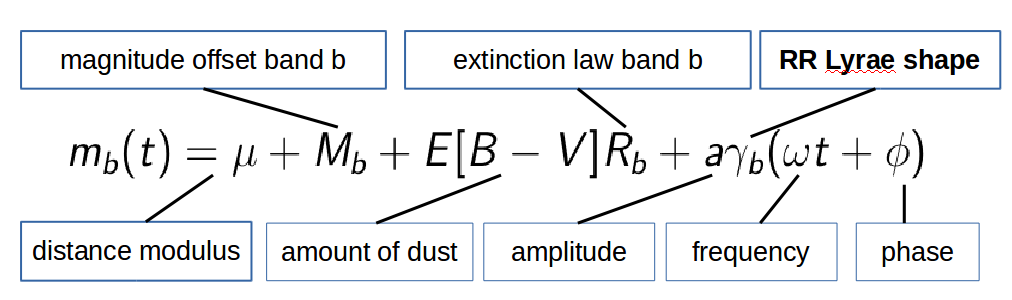
\includegraphics[scale=.3]{figs/model.png}\\
individual parameters fit for each RR Lyrae
\end{center}

\vspace{.2in}

\begin{itemize}
\item $D=\{\{t_{jb},m_{jb},\sigma_{jb}\}_{j=1}^{n_b}\}_{b=1}^B$
\item Model:
\begin{equation*}
m_{jb} = m_b(t_{jb}) + \epsilon_{jb}
\end{equation*}
where $\epsilon_{jb} \sim N(0,\sigma_{jb}^2)$.
\end{itemize}
\end{frame}

\begin{frame}{$\gamma_b$ Estimated from SDSS Stripe 82 RR Lyrae}

\begin{center}
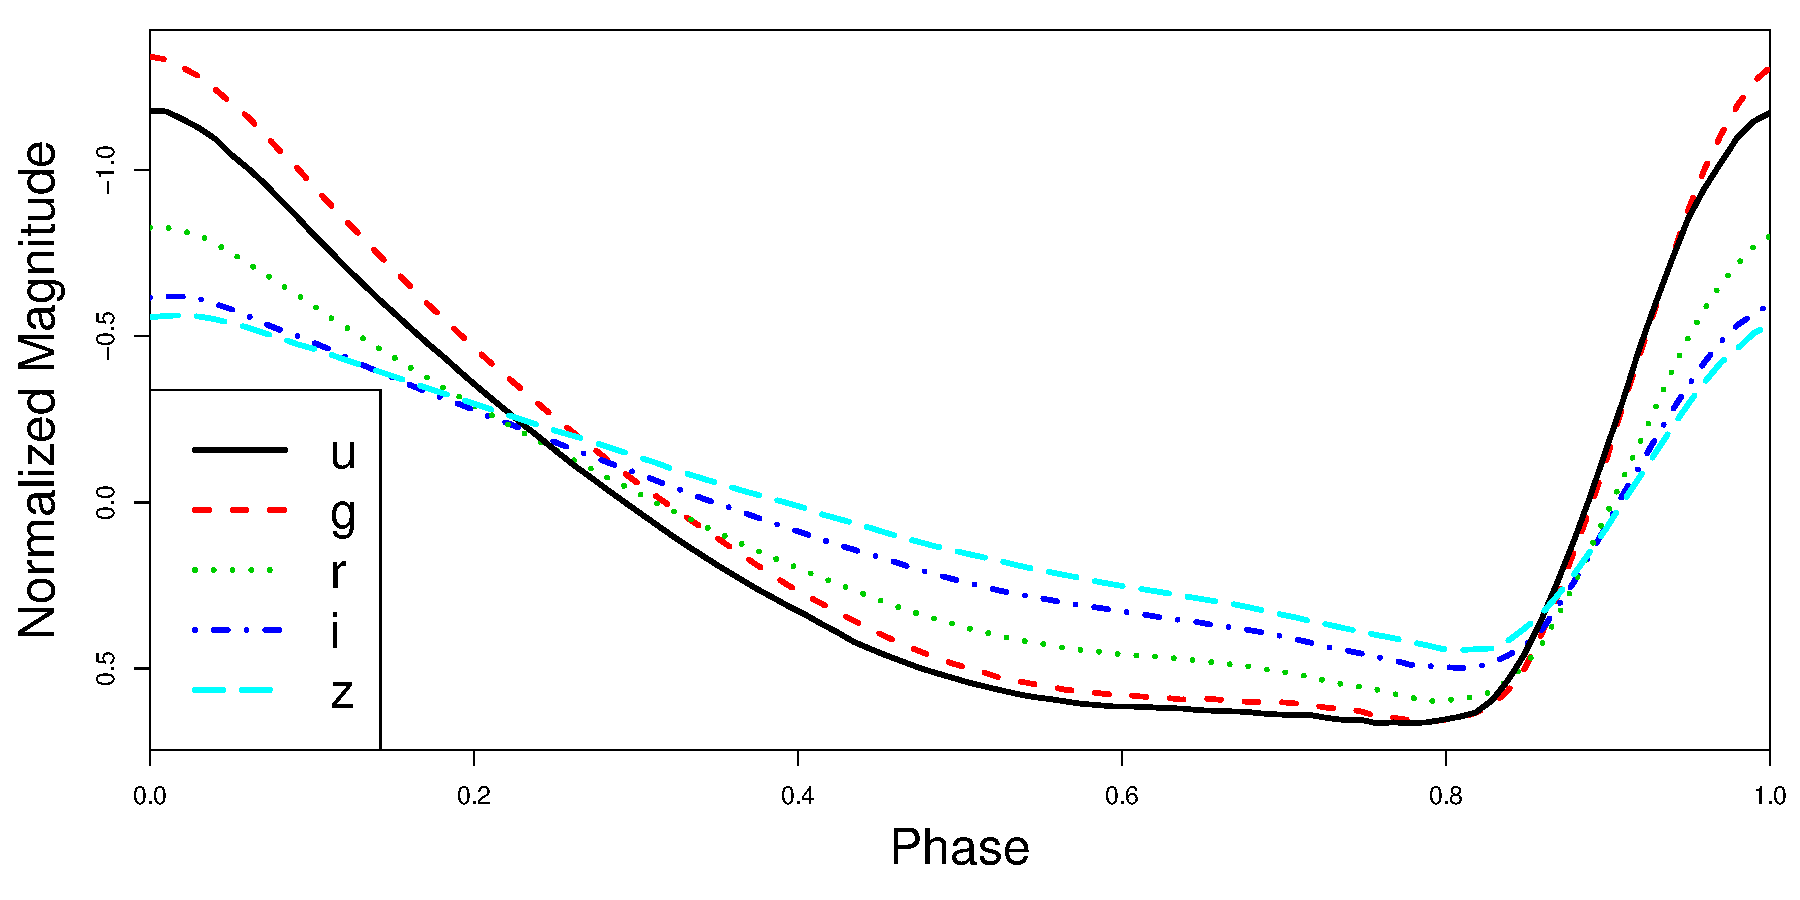
\includegraphics[scale=.3]{figs/templates.pdf}
\end{center}

\end{frame}

\begin{frame}{Parameter Estimation}
%%\begin{itemize}
%% \item Likelihood:
%% \begin{equation*}
%% m_{jb} = m_b(t_{jb}) + \epsilon_{jb} 
%% \end{equation*}
%% where $\epsilon_{jb} \sim N(0,\sigma_{jb}^2)$.
%% \item Define
%% \begin{align*}
%% &RSS(\omega,\mu,E[B-V],a,\phi) \\
%%  &\equiv\sum_{b=1}^B \sum_{j=1}^{n_b}\left(\frac{m_{jb} - \mu - M_b - E[B-V]R_b - a\gamma_b(\omega t_{jb} + \phi)}{\sigma_{bi}}\right)^2
%% \end{align*}
%% \end{itemize}
\begin{align*}
&RSS(\omega,\mu,E[B-V],a,\phi) \\
 &\equiv\sum_{b=1}^B \sum_{j=1}^{n_b}\left(\frac{m_{jb} - \mu - M_b - E[B-V]R_b - a\gamma_b(\omega t_{jb} + \phi)}{\sigma_{jb}}\right)^2
\end{align*}


Estimate parameters with maximum likelihood ($\chi^2$ minimization):
\begin{itemize}
\item Likelihood is highly multimodal in $\omega$, grid search.
\item Model is linear in $\mu$,$E[B-V]$, and $a$, closed form updates.
\item Warm start Newton--Raphson updates for $\phi$.
\end{itemize}

\end{frame}

\begin{frame}{Example Fits to SDSS Light Curves}

\end{frame}

\begin{frame}{Example Fits to DES Light Curves}

\end{frame}

\begin{frame}{Summary of Fitting}

  \todo{State: don't use error variance because worried about model misspecification. mention carroll's article on when measurement errors are estiamte, even more suspicious.} 
  
\end{frame}



%% \begin{frame}{Visualization of Warm Start for $\phi$}

%% \end{frame}

\section{Results on SDSS Stripe 82 and DES}


\subsection{SDSS Stripe 82}

\begin{frame}{Simulate SDSS Stripe 82 to Resemble DES}

  \begin{textblock*}{12cm}(.5cm,2cm) % {block width} (coords)
Downsample Stripe 82 variables to 20 observations across all bands:
\end{textblock*}

  \begin{textblock*}{3cm}(1cm,3.1cm) % {block width} (coords)
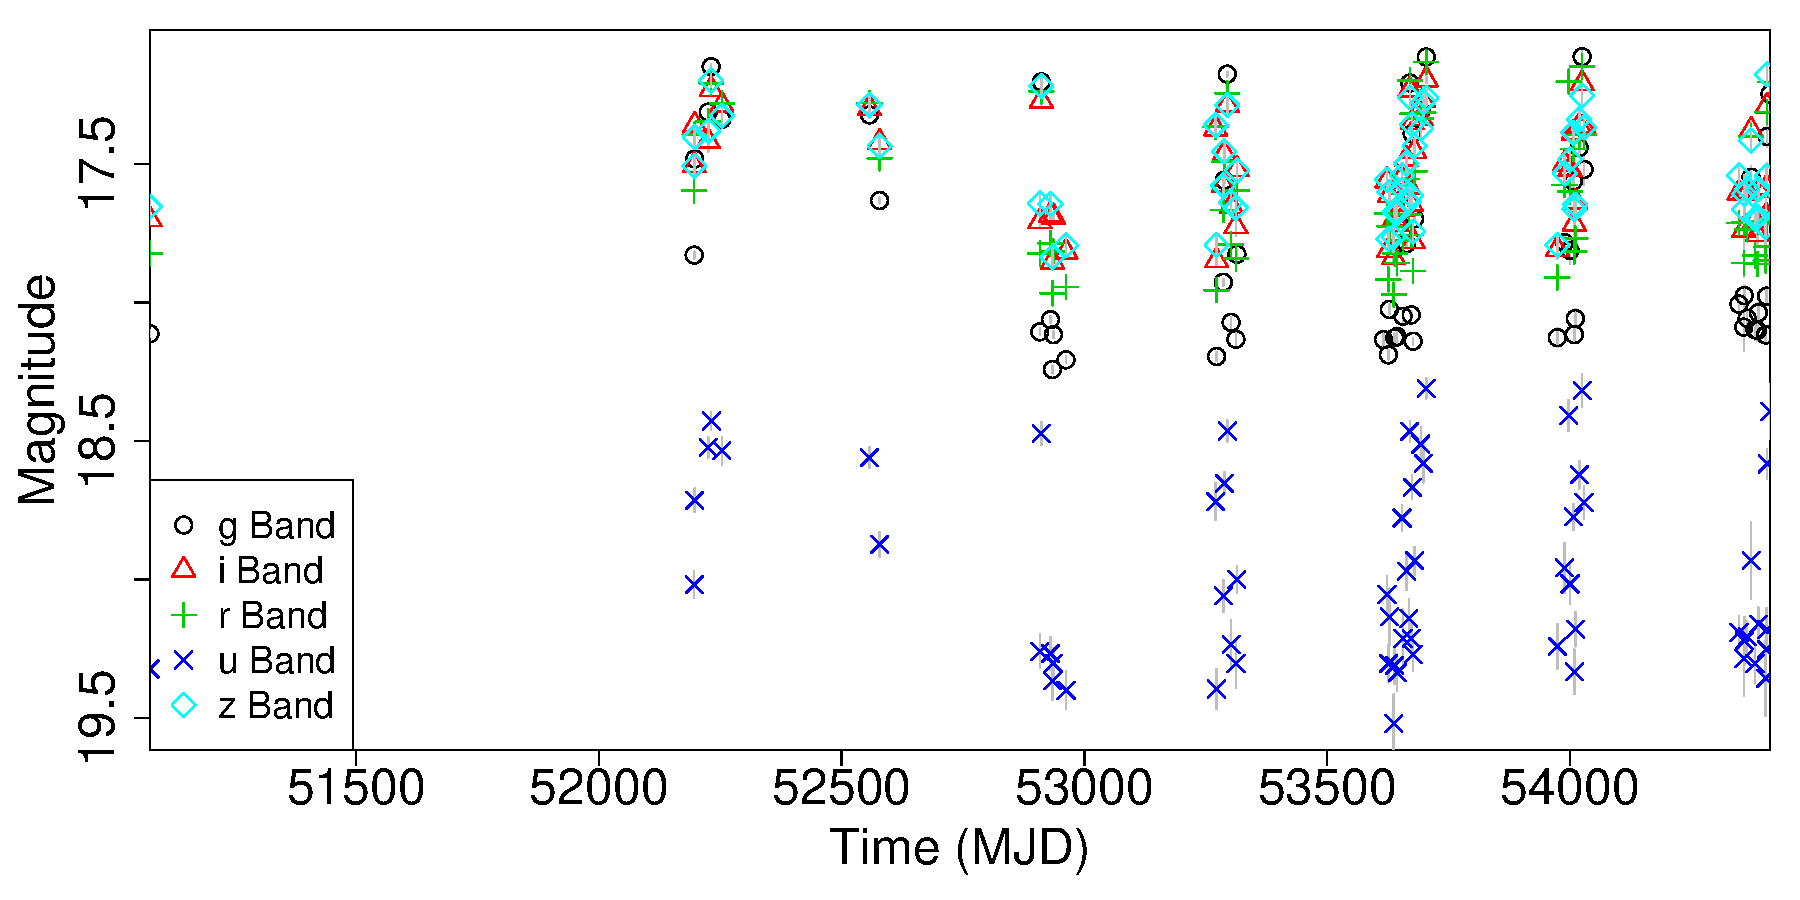
\includegraphics[scale=.15]{figs/unfolded_13350.pdf}
\end{textblock*}


  \begin{textblock*}{3cm}(5.5cm,3.5cm) % {block width} (coords)
\includegraphics[scale=.15]{figs/rightarrow.png}
\end{textblock*}

  \begin{textblock*}{3cm}(6.75cm,3.1cm) % {block width} (coords)
\includegraphics[scale=.15]{figs/unfolded_13350down.pdf}
\end{textblock*}

  \begin{textblock*}{12cm}(1.75cm,6.1cm) % {block width} (coords)
\begin{itemize}
\item Can we estimate periods correctly for RR Lyrae?
\item Can we estimate distances accurately?
\item Can we separate RR Lyrae from non--RR Lyrae? 
\item Can we reproduce halo maps of Sesar 2010?
\end{itemize}
\end{textblock*}

\end{frame}


\begin{frame}{Results for Period Estimation}



\begin{center}
Comparison of period estimates for 350 RR Lyrae\\
\includegraphics[scale=.25]{figs/period_comparison.pdf}
\end{center}


%% \begin{itemize}
%% \item Sine Model: $6$\% of estimates within $0.01$\% of truth.
%% \item RR Lyrae Model: $67$\% of estimates within $0.01$\% of truth.
%% \end{itemize}

\end{frame}


\begin{frame}{Simulation Results for Distance Estimation}
\begin{itemize}
\item Use model to estimate distance modulus ($\mu$) for RR Lyrae.
\item Convert $\mu$ to distance (d) in parsecs: $d = 10^{\mu/5 + 1}$
\end{itemize}

\begin{center}
\includegraphics[scale=.35]{figs/distance_comparison.pdf}
\end{center}



\end{frame}


\begin{frame}{Results for Classification}

\begin{center}
Downsampled 1000 Not--RR Lyrae and 350 RR Lyrae
\includegraphics[scale=.33]{figs/period_vs_EBV.pdf}
\includegraphics[scale=.33]{figs/a_vs_dev_log.pdf}
\end{center}

\begin{itemize}
\item Visually good separation with small number of features.
\item Potential to use model output as feature input to classifier.
%\item Hernitschek \cite{hernitschek2016finding} used structure functions to classify sparsely sampled RR Lyrae in Pan--STARRS.
\end{itemize}
\end{frame}

%% \begin{frame}{Results for Constructing Milky Way Halo Maps}
%%   \def \tw {.1}
  
%%   \begin{figure}[t]
%% %\begin{center}
%%   %\centering
%%   \begin{minipage}{0.5\textwidth}
%%  \subfloat[RRL Locations, SDSS Stripe 82]{\label{fig:density_true_points}
%%  \includegraphics[scale=\tw]{figs/density_true_points.png}
%%  %  \rule{4cm}{3cm}`
%%  }\\
%%  \subfloat[Overdensities, SDSS Stripe 82]{\label{fig:density_true}
%%  \includegraphics[scale=.1]{figs/density_true.png}
%%  %  \rule{4cm}{3cm}`
%%  }
%%   \end{minipage}

  
%% %  \hspace{\fill}
%%   \begin{minipage}{0.5\textwidth}
%%  \subfloat[RRL Location, Downsampled SDSS Stripe 82]{\label{fig:density_rr_model_sampled_points}
%%  \includegraphics[scale=.1]{figs/density_rr_model_sampled_points.png}
%% %   \rule{4cm}{3cm}
%%  }\\
%%     \subfloat[Overdensities, Downsampled SDSS Stripe 82]{\label{fig:density_rr_model_sampled}
%%  \includegraphics[scale=.1]{figs/density_rr_model_sampled.png}
%% %   \rule{4cm}{3cm}
%%  }
%%  \end{minipage}
%% \caption{(a) Location of RRL stars in SDSS Stripe 82. The light curves used to make this map were well sampled so the classifications and distance estimates are quite accurate (i.e. all black points are actually RRL and their location on this map is close to their true location) (b) Overdensities (relative to the oblate MW halo model) represented by redder regions.   (c) The same map in (a) but constructed using poorly sampled light curves. Some of the classifications are incorrect (i.e. some black points are not in fact RRL) and distances contain more scatter. (d) The overdensities determined using sparsely sampled light curves.}
%% %\end{center}
%% \end{figure}


%% \end{frame}





\begin{frame}{Classification Process}
  \todo{describe classification setup here}
\end{frame}


\begin{frame}{Results for Constructing Milky Way Halo Maps}
  \def \tw {.1}
  
  \begin{columns}
    \begin{column}{0.5\textwidth}
      \begin{center}
        \includegraphics[scale=\tw]{figs/density_true_points.png}\\
        RRL Locations, SDSS\\
        \includegraphics[scale=\tw]{figs/density_true.png}\\
        Overdensities, SDSS
      \end{center}
  \end{column}

    \begin{column}{0.5\textwidth}
      \begin{center}
    \includegraphics[scale=\tw]{figs/density_rr_model_sampled_points.png}\\
    RRL Locations, Downsampled\\
    \includegraphics[scale=\tw]{figs/density_rr_model_sampled.png}\\
    Overdensities, Downsampled
    \end{center}
  \end{column}

\end{columns}
\end{frame}




\subsection{Dark Energy Survey}

\begin{frame}{DES Overview}
\todo{describe survey briefly}
\end{frame}


\begin{frame}{FORNAX Dwarf Spheroid Satellite Galaxy}
  \begin{center}
    \includegraphics[scale=0.04]{figs/Fornax_dwarf_galaxy.jpg}
  \end{center}
\att{Wikipedia: \url{https://upload.wikimedia.org/wikipedia/commons/4/45/Fornax_dwarf_galaxy.jpg}}
\end{frame}

\begin{frame}{Data Challenge}

\end{frame}

\section{Ongoing and Related Work}

\begin{frame}{Related Work}

\textbf{Period Estimation Algorithms / Variable Star Models:}
\begin{itemize}
\item Sinusoid Based Methods
\begin{itemize}
\item Lomb Scargle (LS) \cite{lomb1976least,scargle1982studies}
\item Generalized LS (GLS) \cite{zechmeister2009generalised}
\item Multiband Extensions \cite{vanderplas2015periodograms,long2014estimating}.
\item AoV \cite{schwarzenberg1996fast}
\end{itemize}
\item ``Non--parametric'' methods
\begin{itemize}
\item Phase Dispersion Minimization \cite{stellingwerf1978period}
\item Supersmoother \cite{sesar2010light}
\end{itemize}
\item Template Based Methods
\begin{itemize}
\item RR Lyrae templates by Sesar \cite{sesar2010light}, Kovacs \cite{kovacs2007computation}
\item Cepheid templates by Pejcha \cite{pejcha2012global}, Yoachim \cite{yoachim2009panoply}
\end{itemize}
\end{itemize}

\vspace{.1in}

\textbf{Finding RR Lyrae in Sparsely Sampled Light Curves:}
\begin{itemize}
\item Hernitschek \cite{hernitschek2016finding} uses structure functions to find RRL / QSO.
\end{itemize}


\end{frame}

\begin{frame}{Ongoing Work}
\begin{itemize}
\item Model refinements:
\begin{itemize}
\item $M_b$ dependence on period, metallicity.
\item Bands other than $g,i,u,r,z$
\item Parameterize $\gamma_b$ to account for shape differences across RRL
\end{itemize}
\item Propagate uncertainty to 3D halo density estimate
\begin{itemize}
\item Treat as Inference Problem: Bayesian posterior or frequentist confidence bands. Hierarchical model?
\item Treat as Prediction Problem: Evaluate distance / density estimates using Stripe 82 data or follow--up observations.
\end{itemize}
\item Milky Way Halo maps using DES data
\end{itemize}
\end{frame}

%% \begin{frame}{Conclusions}
%% \begin{itemize}
%% \item Models for specific variable star classes:
%% \begin{itemize}
%% \item Pros: better parameter estimates, improved classification
%% \item Cons: difficult to build, more computation time
%% \end{itemize}
%% \item 
%% \item Survey cadence selection
%% \end{itemize}
%% \end{frame}


\begin{frame}[allowframebreaks]{Bibliography}
%  \def\newblock{\hskip .11em plus .33em minus .07em}
%  \nocite{*}
%\nocite{*}
\bibliographystyle{plain} 
  \tiny{
  \bibliography{refs}}
\end{frame}

\section*{Additional Results}

\begin{frame}{Dependence Assumption}
\todo{write here}
\end{frame}

\begin{frame}{Are uncertainties estimated correctly?}
\todo{show example from SDSS suggesting they are.}
\end{frame}


\begin{frame}{$K=1,2,3$ Misspecified Model Results}
\begin{table}[ht]
\centering
\begin{tabular}{c|cc|cc|cc}
 &   $K=1$ &    & $K=2$ &    & $K=3$ &  \\ 
  \hline
n & $\Sigma^{-1}$ &  $I$ & $\Sigma^{-1}$ &  $I$ & $\Sigma^{-1}$ &  $I$ \\
  \hline10&0.09&0.16&0.13&0.11&0.03&0.03\\20&0.46&0.58&0.63&0.68&0.69&0.77\\30&0.64&0.78&0.71&0.82&0.82&0.86\\40&0.75&0.79&0.80&0.85&0.87&0.92\\\hline
\end{tabular}
\caption{Fraction of periods estimated correctly (within 1\%) using models with $K=1,2,3$ harmonics ($p=4,5,8$ parameters, respectively). Ignoring the observation uncertainties ($I$) in the fitting is superior to using them ($\Sigma^{-1}$). The standard deviation on these accuracies is no larger than $\sqrt{0.5(1-0.5)/238} \approx 0.032$ .}
\label{tab:period_est_results}
\end{table}

\end{frame}


\end{document}
